\documentclass[12pt,a4paper]{report}

% Kódování a jazyk
\usepackage[utf8]{inputenc}
\usepackage[czech]{babel}
\usepackage[T1]{fontenc}

% Písmo — Charter (text) + Source Sans Pro (nadpisy) + matching math
\usepackage{XCharter}
\usepackage[scaled=0.95]{sourcesanspro}
\usepackage[charter,vvarbb]{newtxmath}

% Bezpatkové nadpisy (Helvetica)
\usepackage{titlesec}
\titleformat{\chapter}[display]
  {\normalfont\sffamily\bfseries\LARGE}
  {\chaptertitlename\ \thechapter}{0.5em}{}
\titleformat{\section}
  {\normalfont\sffamily\bfseries\Large}
  {\thesection}{0.5em}{}
\titleformat{\subsection}
  {\normalfont\sffamily\bfseries\large}
  {\thesubsection}{0.5em}{}
\titleformat{\paragraph}[hang]
  {\normalfont\bfseries\normalsize}
  {}{0em}{}
\titlespacing*{\paragraph}{0pt}{1em}{0.5em}

% Grafika a obrázky
\usepackage{graphicx}
\graphicspath{{images/}}

% Matematika (newtxmath obsahuje amsmath i amssymb funkce)

% Landscape stránky (přílohy)
\usepackage{pdflscape}

% Vkládání externích PDF (zadání práce z IS STAG)
\usepackage{pdfpages}

% Odkazy a reference
\usepackage{hyperref}
\hypersetup{
    colorlinks=true,
    linkcolor=black,
    citecolor=blue,
    urlcolor=blue
}

% Formátování stránky
\usepackage[left=3.5cm,right=2cm,top=2cm,bottom=2cm]{geometry}
\usepackage{setspace}
\onehalfspacing

% Diagramy
\usepackage{tikz}
\usetikzlibrary{arrows.meta, positioning, shapes.geometric, calc, backgrounds, fit}
\usepackage{pgfplots}
\pgfplotsset{compat=1.18}
\usepackage{float}

% Výpisy kódu
\usepackage{listings}
\usepackage{xcolor}

% Nastavení výpisů kódu
\lstset{
    basicstyle=\ttfamily\small,
    keywordstyle=\color{blue}\bfseries,
    commentstyle=\color{green!60!black},
    stringstyle=\color{red},
    showstringspaces=false,
    breaklines=true,
    frame=single,
    numbers=left,
    numberstyle=\tiny\color{gray},
    captionpos=b
}

% Bibliografie
\usepackage[style=iso-numeric,backend=biber]{biblatex}
\addbibresource{bibliography.bib}

% Metadata a titulní stránka
% Metadata bakalářské práce

% Univerzita a fakulta
\def\university{Univerzita Hradec Králové}
\def\faculty{Fakulta informatiky a managementu}
\def\department{Katedra informatiky a kvantitativních metod}

% Informace o práci
\def\thesistype{Bakalářská práce}
\def\thesistitle{Interaktivní platforma pro prezentaci činnosti raketového spolku}
\def\thesistitleEN{Interactive platform for presenting activities of a rocket club}

% Autor
\def\author{Šimon Cerman}
\def\authorid{I2300268}

% Vedoucí práce
\def\supervisor{Petr Bauer, Ph.D.}
\def\supervisortitle{Ing.}

% Datum
\def\thesisyear{2026}
\def\submissiondate{20. dubna 2026}

% Klíčová slova (doporučený počet 5)
\def\keywords{webová platforma, raketový spolek, telemetrie, MQTT, monorepo}
\def\keywordsEN{web platform, rocket club, telemetry, MQTT, monorepo}


\begin{document}

% Titulní stránka
\begin{titlepage}
    \centering

    \vspace*{0.5cm}

    {\Large \university \par}
    {\Large \faculty \par}
    {\large \department \par}

    \vspace{4cm}

    {\huge\bfseries \thesistitle \par}

    \vspace{0.8cm}

    {\Large \thesistype \par}

    \vfill

    \begin{flushleft}
        {\large
        Autor: \author \\
        Studijní program: Aplikovaná informatika \\
        Specializace: Softwarové inženýrství \\[1em]
        Vedoucí práce: \supervisortitle~\supervisor \\
        \phantom{Vedoucí práce: }Katedra informatiky a~kvantitativních metod \\
        }
    \end{flushleft}

    \vspace{1cm}

    \noindent
    {\large Hradec Králové \hfill \thesisyear \par}

\end{titlepage}


% Čestné prohlášení
\chapter*{Prohlášení}

Prohlašuji, že jsem tuto bakalářskou práci vypracoval samostatně a~uvedl jsem všechny použité prameny a~literaturu. V~případě využití nástrojů umělé inteligence jsem plně deklaroval způsob jejich využití při vypracování této práce.

\vspace{4em}

\noindent
V Hradci Králové dne \submissiondate \hfill \author

\vspace{3em}

\noindent
\hfill \makebox[5cm]{\dotfill}

\clearpage


% Poděkování
\chapter*{Poděkování}

Rád bych poděkoval vedoucímu práce \supervisortitle~\supervisor{} za odborné vedení, trpělivost a~cenné připomínky při zpracování této bakalářské práce. Dále děkuji členům spolku Czech Rocket Society za spolupráci při specifikaci požadavků a~testování výsledné platformy.

\clearpage


% Abstrakt
\chapter*{Abstrakt}
\begin{sloppypar}
Tato bakalářská práce se zabývá návrhem a~implementací interaktivní webové platformy pro studentský raketový spolek Czech Rocket Society. Cílem bylo vytvořit moderní aplikaci nahrazující stávající statický web, která umožní správu obsahu bez programátorských znalostí, digitalizuje náborový proces a~poskytne nástroje pro vizualizaci telemetrických dat z~raketových letů v~reálném čase.
\end{sloppypar}

Architektura platformy je složena ze~tří aplikací v~monorepo struktuře: frontend v~Next.js se~serverovým vykreslováním, REST API backend postavený na~frameworku Hono s~ORM Drizzle a~databází PostgreSQL a~telemetrický server v~Go zpracovávající data přenášená protokolem MQTT a~ukládaná do~časové databáze InfluxDB.

Výsledkem je funkční aplikace zahrnující veřejný web, administrační CMS, vícekrokový náborový formulář s~průběžným ukládáním a~e-mailovými notifikacemi a~telemetrický dashboard s~dvoukanálovým příjmem dat a~přehráváním historických záznamů. Aplikace byla ověřena sadou automatizovaných unit a~integračních testů i~manuálním testováním. Celé řešení je kontejnerizováno pomocí Docker Compose a~připraveno k~nasazení do produkčního prostředí spolku.

\vspace{1em}
\noindent\textbf{Klíčová slova:} \keywords

\chapter*{Abstract}

\noindent\textbf{Title: \thesistitleEN}

\vspace{1em}

\noindent This bachelor thesis deals with the design and implementation of an interactive web platform for the student rocketry club Czech Rocket Society. The goal was to create a~modern application replacing the existing static website, enabling content management without programming knowledge, digitizing the recruitment process and providing tools for real-time visualization of telemetric data from rocket flights.

The platform architecture consists of three applications in a~monorepo structure: a~Next.js frontend with server-side rendering, a~REST API backend built on the Hono framework with Drizzle ORM and a~PostgreSQL database, and a~telemetry server written in Go processing data transmitted via the MQTT protocol and stored in the InfluxDB time-series database.

The result is a~functional application comprising a~public website, an administrative CMS, a~multi-step recruitment form with auto-save and email notifications, and a~telemetry dashboard with dual-channel data reception and historical data playback. The application was verified by a~suite of automated unit and integration tests as well as manual testing. The entire solution is containerized using Docker Compose and ready for deployment in the club's production environment.

\vspace{1em}
\noindent\textbf{Keywords:} \keywordsEN

\clearpage

% Obsah
\tableofcontents
\clearpage

% Seznam obrázků
\listoffigures
\clearpage

% Seznam tabulek
\listoftables
\clearpage

% Seznam zkratek
\chapter*{Seznam zkratek}
\addcontentsline{toc}{chapter}{Seznam zkratek}

\begin{tabbing}
\hspace{3cm} \= \kill
ACID \> Atomicity, Consistency, Isolation, Durability \\
AI \> Artificial Intelligence (umělá inteligence) \\
API \> Application Programming Interface \\
CI/CD \> Continuous Integration / Continuous Deployment \\
CMS \> Content Management System (systém správy obsahu) \\
CORS \> Cross-Origin Resource Sharing \\
CRS \> Czech Rocket Society \\
CRUD \> Create, Read, Update, Delete \\
CSS \> Cascading Style Sheets \\
CSV \> Comma-Separated Values \\
DOM \> Document Object Model \\
ESA \> European Space Agency (Evropská kosmická agentura) \\
ESM \> ECMAScript Modules \\
GPS \> Global Positioning System \\
HMAC \> Hash-based Message Authentication Code \\
HTML \> Hypertext Markup Language \\
HTTP \> Hypertext Transfer Protocol \\
HTTPS \> Hypertext Transfer Protocol Secure \\
I/O \> Input/Output (vstup/výstup) \\
IoT \> Internet of Things (internet věcí) \\
ISR \> Incremental Static Regeneration \\
JSON \> JavaScript Object Notation \\
JSONB \> JSON Binary \\
JWT \> JSON Web Token \\
LLM \> Large Language Model (velký jazykový model) \\
MIME \> Multipurpose Internet Mail Extensions \\
MQTT \> Message Queuing Telemetry Transport \\
ORM \> Object-Relational Mapping \\
PHP \> PHP: Hypertext Preprocessor \\
PWA \> Progressive Web App \\
QoS \> Quality of Service (kvalita doručení) \\
RBAC \> Role-Based Access Control \\
REST \> Representational State Transfer \\
RFC \> Request for Comments \\
SEO \> Search Engine Optimization (optimalizace pro vyhledávače) \\
SMTP \> Simple Mail Transfer Protocol \\
SPA \> Single Page Application \\
SQL \> Structured Query Language \\
SSE \> Server-Sent Events \\
SSG \> Static Site Generation \\
SSR \> Server-Side Rendering \\
SVG \> Scalable Vector Graphics \\
TCP \> Transmission Control Protocol \\
TSM \> Time-Structured Merge Tree \\
URL \> Uniform Resource Locator \\
UUID \> Universally Unique Identifier \\
VPS \> Virtual Private Server \\
WSS \> WebSocket Secure \\
YAML \> YAML Ain't Markup Language \\
\end{tabbing}

\clearpage

% Kapitoly
\chapter{Úvod}

\section{Motivace}
Téma bakalářské práce bylo zvoleno na~základě potřeb studentského raketového spolku Czech Rocket Society jak z~hlediska popularizace kosmonautiky v~České republice, tak pro~vnitřní fungování spolku.
Platforma je navržena jako nástroj, který umožní lépe prezentovat reálné schopnosti studentů působících v~kosmickém raketovém sektoru, včetně možnosti zobrazovat živá telemetrická data z~letů raket. Součástí jsou také menší podpůrné aplikace pro každodenní činnost spolku.
Cílem je vytvořit modulární platformu složenou z~několika subsystémů, z~nichž každý podporuje konkrétní spolkovou činnost a~činí ji efektivnější.
Aplikace přináší nejen nové funkcionality, ale také částečně řeší problémy stávajícího webu. Ten je postaven na~technologiích, které neumožňují jednoduchou údržbu obsahu ani jeho aktualizace bez hlubší znalosti programovacích či značkovacích jazyků a~základů systémů správy verzí.
Po~designové stránce by měl web splňovat nároky spolku, obstát ve~srovnání s~konkurencí a~vhodně propagovat kosmonautiku v~České republice.

\section{Struktura práce}
Práce je rozdělena do následujících kapitol:
\begin{itemize}
    \item \textbf{Cíl a~metodika práce} -- vymezení cílů, popis zvolené metodiky a~využití nástrojů umělé inteligence.
    \item \textbf{Teoretická část a~analýza} -- analýza domény, přehled existujících řešení a~teoretický základ použitých technologií.
    \item \textbf{Návrh řešení} -- architektura systému, datový model, návrh API (Application Programming Interface) a~uživatelského rozhraní.
    \item \textbf{Implementace} -- popis realizace jednotlivých částí platformy.
    \item \textbf{Testování} -- metodika testování a~shrnutí výsledků.
    \item \textbf{Shrnutí a~diskuse výsledků} -- porovnání s~výchozím stavem, soulad výsledků s~literaturou a~okolnosti ovlivňující průběh práce.
    \item \textbf{Závěry a~doporučení} -- zhodnocení splnění cílů a~možnosti budoucího rozvoje.
\end{itemize}
\chapter{Cíl a metodika práce}

\section{Hlavní cíl}
Cílem bakalářské práce bylo vytvoření webové aplikace s~více funkcionalitami pro širší pokrytí potřeb spolku v~rámci webové prezentace a~zároveň pro vybudování dobrého základu, na kterém by mohli stavět další členové spolku.

Nejviditelnější částí webové aplikace je samotný web s~moderním a~přehledným designem postaveným z~komponent pro snadnou práci s~ním i~v~budoucích letech. Součástí je také náborový dotazník, aktuality a~další části webu nepostradatelné pro prezentaci raketového spolku.

Druhou částí je separátní backendová vrstva, která zajišťuje rozšířenou funkcionalitu -- primárně přenos dat ze~vzdálených testovacích míst a~pozemních stanic, jednak pro přehlednost činností, jednak pro zajištění bezpečnosti.

\section{Dílčí cíle}

Pro dosažení hlavního cíle jsou stanoveny následující dílčí cíle:

\begin{enumerate}
    \item \textbf{Veřejný web s~moderním designem} -- implementace responzivního webu se serverovým vykreslováním (SSR) pro optimalizaci načítání a~indexaci vyhledávači.
    \item \textbf{Administrační systém pro správu obsahu} -- rozhraní umožňující členům spolku spravovat články, události, projekty, členy a~partnery bez nutnosti programátorských znalostí.
    \item \textbf{Interaktivní náborový formulář} -- vícekrokový formulář s~průběžným ukládáním rozpracovaných přihlášek, e-mailovými notifikacemi a~administračním workflow pro správu uchazečů.
    \item \textbf{Telemetrický systém} -- systém pro příjem, ukládání a~vizualizaci telemetrických dat z~raketových letů v~reálném čase, včetně přehrávání historických dat a~simulátoru pro testování.
    \item \textbf{Autentizace a~zabezpečení platformy} -- přihlašování do administrace, ochrana API endpointů a~bezpečné ukládání citlivých údajů.
    \item \textbf{Testování a~ověření funkčnosti} -- ověření správnosti aplikace automatizovanými testy (unit, integrační) i~manuálním testováním klíčových scénářů.
\end{enumerate}

\section{Metodika}
Práce probíhala v~několika fázích zahrnujících analýzu požadavků, návrh architektury, implementaci a~testování aplikace.
Analýza potřeb spolku proběhla prostřednictvím několika meetingů a~společného brainstormingu. Na těchto setkáních došlo ke zpřesnění požadavků a~ujasnění funkcionalit, které by měla aplikace obsahovat, aby byla spolku užitečnou komponentou.

Aplikace byla vyvíjena iterativním přístupem, tedy průběžným prototypováním a~postupnou prací na~jednotlivých částech~\cite{nolle2020waterfall}. Toho bylo dosaženo díky rozdělení aplikace na logické části, které bylo možné testovat nezávisle na zbytku systému, případně nasazovat jednotlivě.
Komponenty byly testovány jak jednotkovými testy, tak integračními testy i~uživatelským testováním.

Pro testování telemetrického systému bez nutnosti fyzického startu je využíván simulátor generující realistická data. Do budoucna se počítá s~ověřením systému při reálných startech.

Jelikož aplikace bude používána spolkem i~v~příštích letech, bylo dbáno na čitelnost kódu a~komentáře, aby bylo možné do aplikace v~budoucnosti přispívat. Tato bakalářská práce slouží jako popis architektury a~návrhových rozhodnutí, technická dokumentace API je generována automaticky nástrojem Swagger~UI.

\section{Využití umělé inteligence ve vývojovém procesu}
Integrace nástrojů založených na~velkých jazykových modelech (LLM) do~vývojového procesu představuje jeden z~nejvýraznějších trendů současného softwarového inženýrství. Systematický přehled 39~studií z~let 2014--2024, z~nichž 73\,\% bylo publikováno teprve v~roce 2024, dokládá rychle rostoucí zájem o~tuto oblast~\cite{mohamed2025llmproductivity}. Výzkumy ukazují, že LLM asistenti urychlují vývoj automatizací opakujících se úkonů, snižují potřebu vyhledávání řešení v~externích zdrojích a~pomáhají vývojářům udržet soustředění při práci. Empirické studie uvádějí zlepšení produktivity vývoje řádově v~desítkách procent. Zároveň však literatura upozorňuje, že zvýšená rychlost nemusí vždy korelovat s~kvalitou -- některé studie zaznamenaly trade-off mezi propustností a~kvalitou kódu, což podtrhuje důležitost průběžné revize generovaných výstupů~\cite{mohamed2025llmproductivity}.

V~průběhu vývoje této bakalářské práce byly nástroje umělé inteligence (AI) využity k~podpoře různých aspektů vývojového procesu s~cílem zvýšit efektivitu a~usnadnit řešení komplexních problémů. Generované výstupy byly vždy podrobeny manuální kontrole a~úpravám. V~souladu se směrnicí FIM UHK jsou níže uvedeny konkrétní nástroje, jejich verze a~rozsah využití.

\paragraph{Použité nástroje}

\begin{itemize}
    \item \textbf{Claude Code} (Anthropic, modely Claude Opus 4.5/4.6 a~Claude Sonnet 4.5) -- agentní CLI nástroj pro práci v~terminálu. Hlavní nástroj využívaný v~průběhu celého vývoje. Sloužil ke~generování kódu, refaktoringu, hromadným změnám napříč projektem, tvorbě testů, revizi kódu a~hledání chyb. Rovněž byl využit při korekturách textu bakalářské práce. Rozsah využití: vysoký -- využíván průběžně po~celou implementační fázi.

    \item \textbf{GitHub Copilot} (GitHub, využívající modely Claude Sonnet~3.7, GPT a~další) -- doplněk do~editoru VS~Code poskytující průběžné návrhy kódu při~psaní. Využíván jako kontextový našeptávač pro dokončování řádků a~generování krátkých bloků kódu. Rozsah využití: střední -- aktivní během celého vývoje jako~kontextový našeptávač.

    \item \textbf{Gemini} (Google, řada Gemini~2.5) -- využíván v~rané fázi projektu pro konzultace návrhu architektury, porovnávání technologických alternativ a~vyhledávání vhodných klíčových slov pro rešerši odborných zdrojů. Rozsah využití: nízký -- omezen na~fázi analýzy a~návrhu.

    \item \textbf{NotebookLM} (Google) -- nástroj pro sumarizaci a~analýzu odborných zdrojů. Využíván při zpracování rešerše literatury k~rychlé orientaci v~obsahu zdrojů před jejich důkladným prostudováním. Rozsah využití: nízký -- omezen na rešeršní fázi.
\end{itemize}

\paragraph{Oblasti využití}

AI nástroje byly integrovány do~následujících oblastí vývojového procesu:
\begin{itemize}
    \item \textbf{Analýza požadavků a~návrh architektury:} AI nástroje asistovaly při syntéze požadavků získaných od~členů spolku a~pomáhaly identifikovat klíčové funkcionality. Návrhy architektury byly s~nimi diskutovány za~účelem ověření zvoleného přístupu a~hledání možných vylepšení.

    \item \textbf{Implementace a~refaktoring:} AI asistenti pomáhali s~generováním kódu, tvorbou boilerplate struktur, prováděním hromadných změn napříč projektem (přejmenování, aktualizace závislostí) a~navrhovali zlepšení kvality existujícího kódu.

    \item \textbf{Revize kódu:} AI nástroje sloužily k~průběžné kontrole generovaného i~ručně psaného kódu -- identifikovaly potenciální chyby, bezpečnostní zranitelnosti a~nekonzistence, čímž doplňovaly manuální code review.

    \item \textbf{Testování:} AI pomáhalo s~tvorbou testovacích scénářů, generováním testovacích dat a~analýzou výsledků testů pro odhalení slabých míst v~aplikaci.

    \item \textbf{Texty uživatelského rozhraní:} AI nástroje asistovaly při tvorbě a~úpravě textů zobrazovaných na~webu (popisky, hlášky, navigační prvky).

    \item \textbf{Korektury textu práce:} U~textu bakalářské práce byly AI nástroje využity výhradně ke~korekturám pravopisu, návrhům formulačních úprav a~ověřování srozumitelnosti odborného textu. Samotný obsah a~struktura práce byly zpracovány samostatně.
\end{itemize}

Koncepční rozhodnutí, architektura systému, výběr technologií a~finální podoba implementace byly zpracovány samostatně. Limity AI nástrojů a~konkrétní příklady problémů, které vyžadovaly manuální opravu, jsou diskutovány v~kapitolách~\ref{chap:testovani} a~\ref{chap:diskuse}.

\chapter{Teoretická část a~analýza}
\label{chap:analyza}

\section{Analýza domény}
Aplikace si klade za cíl naplnit potřeby raketového spolku v~oblasti prezentace činností, organizace členů a~sdílení informací o~raketových projektech. Toho dosáhne zefektivněním stávajících procesů, zjednodušením administrace a~zavedením nových nástrojů pro zajištění bezpečnosti při činnostech spolku.

Využívají ji především členové spolku a~zájemci procházející náborovým procesem, ale také veřejnost a~soukromé firmy se zájmem o~kosmonautiku. Aplikace tak slouží i~jako prostředek popularizace oboru v~České republice.

\subsection{Kosmonautika a raketový průmysl}
Raketový průmysl na území České republiky má dlouhou tradici sahající od vojenských programů v~období studené války~\cite{lehky2017rakety} přes civilní raketové modelářství pod záštitou organizace SVAZARM~\cite{kosmo2004modelarstvi} až po současné členství v~Evropské kosmické agentuře (ESA), ke kterému došlo v~roce 2008~\cite{mzv2024space}. Česká republika si dnes buduje pozici aktivního hráče v~evropském kosmickém sektoru, jak dokládá i~Národní kosmický plán na léta 2020--2025~\cite{czechspace2020plan}. S~rostoucím zájmem o~kosmonautiku roste i~potřeba popularizace oboru a~zapojení mladé generace.

\subsection{Czech Rocket Society}
Czech Rocket Society je studentský spolek stojící na pomezí akademického prostředí a~praktického inženýrství, který svou činností doplňuje průmyslové i~vzdělávací iniciativy v~oblasti kosmonautiky~\cite{crs2024onas}. Cílem této práce je poskytnout spolku nástroj pro efektivnější prezentaci projektů, oslovování nových členů a~veřejnosti~\cite{crs2024web}.


\subsection{Požadavky na webovou platformu}

Z analýzy potřeb spolku vyplynulo několik cílových skupin, pro které musí platforma fungovat. Primárně jde o~\textbf{veřejnost}, která hledá informace o~činnosti spolku, dále o~\textbf{potenciální členy}, kteří procházejí náborovým procesem, \textbf{stávající členy} spolku a~v~neposlední řadě \textbf{administrátory}, kteří spravují obsah a~řídí interní procesy.

Z hlediska funkčních požadavků platforma musí umožňovat správu a~publikaci obsahu -- článků, událostí, projektů a~informací o~členech a~partnerech. Důležitou součástí je náborový formulář s~možností průběžného ukládání rozpracovaných přihlášek. Specifickým požadavkem, který odlišuje tuto platformu od běžných prezentačních webů, je modul pro přenášení a~vizualizaci telemetrických dat z~raketových letů v~reálném čase.

Mezi nefunkční požadavky patří responzivní design pro mobilní zařízení a~optimalizace pro vyhledávače (SEO, Search Engine Optimization). Pro zpracování telemetrických dat je nutný dostatečný výkon s~nízkou latencí. Posledním klíčovým požadavkem je rozšiřitelnost platformy umožňující budoucí rozvoj dalšími členy spolku.

\subsection{Telemetrie raketových letů}
Telemetrie představuje soubor dat naměřených senzory rakety v~průběhu letu~\cite{lacek2019rocket}. Tato data jsou klíčová jak pro zpětné vyhodnocení letu, tak pro živý přenos informací operujícímu týmu na~zemi~\cite{nasa2023srhb}.

Telemetrická data mohou zahrnovat širokou škálu měřených veličin -- výšku, zrychlení, polohu pomocí GPS (Global Positioning System), orientaci z~gyroskopu či stav baterie. V~případě raket s~kapalinovým pohonem přibývají další údaje o~stavu nádrže, tlaku paliva a~poloze ventilů~\cite{lacek2019rocket}.

Pozemní tým potřebuje mít k~těmto datům přístup v~reálném čase s~co nejnižší latencí, aby byl schopen včas reagovat na~případné anomálie -- například aktivovat záchranný systém nebo upozornit okolí na~hrozící nebezpečí~\cite{kaknjo2019lowcost}. Bezpečnostní pravidla pro provoz amatérských raket, jako je například kodex Tripoli Rocketry Association~\cite{tripoli2025safety}, kladou důraz na~kontrolu letu i~na~vyhrazení vzdušného prostoru, který je v~České republice regulován Úřadem pro civilní letectví~\cite{caa2023lkr10}. Samotný přístup k~surovým datům však nestačí; data musí být přehledně zpracována a~vizualizována tak, aby je operátor dokázal rychle vyhodnotit a~na~jejich základě rozhodnout~\cite{nasa2023srhb}.


\section{Přehled existujících řešení}

\subsection{Stávající telemetrické řešení spolku}
Před vznikem této práce spolek disponoval jednoduchým telemetrickým systémem postaveným na dvou PHP (PHP: Hypertext Preprocessor) skriptech a~vzdálené MySQL databázi. Architektura fungovala následovně: pozemní stanice při příjmu dat z~rakety odeslala HTTP (Hypertext Transfer Protocol) POST požadavek na serverový skript, který přijatá data zapsal do jediného záznamu v~databázové tabulce. Klientská zařízení poté opakovaně a~v~co nejkratších intervalech četla tento záznam pomocí druhého skriptu, který vracel poslední vložený řádek.

Architektura tohoto řešení je znázorněna na obrázku~\ref{fig:old-telemetry}.

\begin{figure}[ht]
\centering
\begin{tikzpicture}[
    node distance=2.0cm and 2.2cm,
    box/.style={rectangle, draw, rounded corners, minimum height=1.1cm, minimum width=2.6cm, align=center, font=\small},
    arrow/.style={-{Stealth[length=3mm]}, thick},
    label/.style={font=\footnotesize, fill=white, inner sep=2pt}
]
    % Nodes - top row
    \node[box] (rocket) {Raketa\\{\footnotesize (senzory)}};
    \node[box, right=of rocket] (ground) {Pozemní\\stanice};
    \node[box, right=of ground] (php) {PHP skript\\{\footnotesize (webový server)}};

    % Nodes - bottom row
    \node[box, below=2.2cm of ground] (client) {Klientská\\zařízení};
    \node[box, below=2.2cm of php] (db) {MySQL\\databáze};

    % Write flow (top + right side)
    \draw[arrow, dashed] (rocket) -- node[label, above=8pt] {rádiový signál} (ground);
    \draw[arrow] (ground) -- node[label, above=8pt] {HTTP POST} (php);
    \draw[arrow] ($(php.south)+(0.25,0)$) -- node[label, right] {INSERT} ($(db.north)+(0.25,0)$);

    % Read flow (bottom + left side)
    \draw[arrow] (php) -- node[label, above, align=center] {HTTP GET\\ {\footnotesize (polling)}} (client);
    \draw[arrow] ($(db.north)+(-0.25,0)$) -- node[label, left] {SELECT} ($(php.south)+(-0.25,0)$);
\end{tikzpicture}
\caption{Architektura stávajícího telemetrického řešení spolku.}
\label{fig:old-telemetry}
\end{figure}

Toto řešení trpělo několika zásadními nedostatky. Přenos dat fungoval na principu pollingu -- klient musel neustále odesílat HTTP dotazy na server, aby zjistil, zda jsou k~dispozici nová data. Každý takový dotaz znamenal navázání nového připojení k~databázi, provedení SQL (Structured Query Language) dotazu a~uzavření spojení, což představovalo zbytečnou zátěž jak na server, tak na databázi. Latence celého řetězce závisela na frekvenci dotazování a~na odezvě vzdálené databáze.

Systém rovněž neuchovával historii měření a~neumožňoval zpětnou analýzu letu. Z~hlediska bezpečnosti obsahoval přístupové údaje k~databázi přímo ve zdrojovém kódu a~autentizace probíhala pomocí statického hesla v~HTTP hlavičce.

Tyto zkušenosti z~praxe přímo motivovaly návrh nového řešení postaveného na moderních technologiích, které jsou popsány v~následujících kapitolách.

\subsection{Stávající webová prezentace spolku}
Současný web spolku\footnote{\url{https://czechrockets.com}} je postaven jako sada statických HTML (Hypertext Markup Language) stránek. Obsahuje základní sekce -- úvodní stránku, představení spolku a~správní rady, přehled projektů, média, partnery a~kontaktní informace~\cite{crs2024web}. Úvodní stránka stávajícího webu je zachycena na obrázku~\ref{fig:crs-current-web}. Design je čistý a~přehledný, stránky však postrádají jakoukoli dynamičnost -- veškerý obsah je pevně zapsán přímo ve zdrojovém kódu a~jeho aktualizace vyžaduje ruční úpravu HTML souborů a~opětovné nasazení.

To v~praxi znamená, že přidání nového článku, úprava informací o~členech rady nebo aktualizace projektových stránek je vázána na člena spolku se znalostí webového vývoje. Obsah webu tak postupně zastarává a~neodpovídá aktuálnímu stavu činností spolku.

Náborový proces je řešen externím formulářem na platformě JotForm, na který odkazuje stránka pro zájemce. Tato stránka sice obsahuje přehled jednotlivých odborů a~odpovědi na~časté dotazy, samotný formulář je však oddělený od~zbytku webu a~neumožňuje například průběžné ukládání rozpracované přihlášky ani správu přijatých žádostí.

Nové řešení si klade za cíl tyto nedostatky odstranit -- zavést systém správy obsahu umožňující aktualizaci bez programátorských znalostí, implementovat interaktivní náborový formulář s~možností průběžného ukládání a~správy přihlášek, poskytnout přehled členů a~partnerů spolku a~celkově nabídnout moderní design, který spolek vhodně reprezentuje.

Podrobné srovnání stávajícího a~nového řešení z~hlediska výkonu a~funkcionality je provedeno v~kapitole věnované testování.

\begin{figure}[ht]
\centering
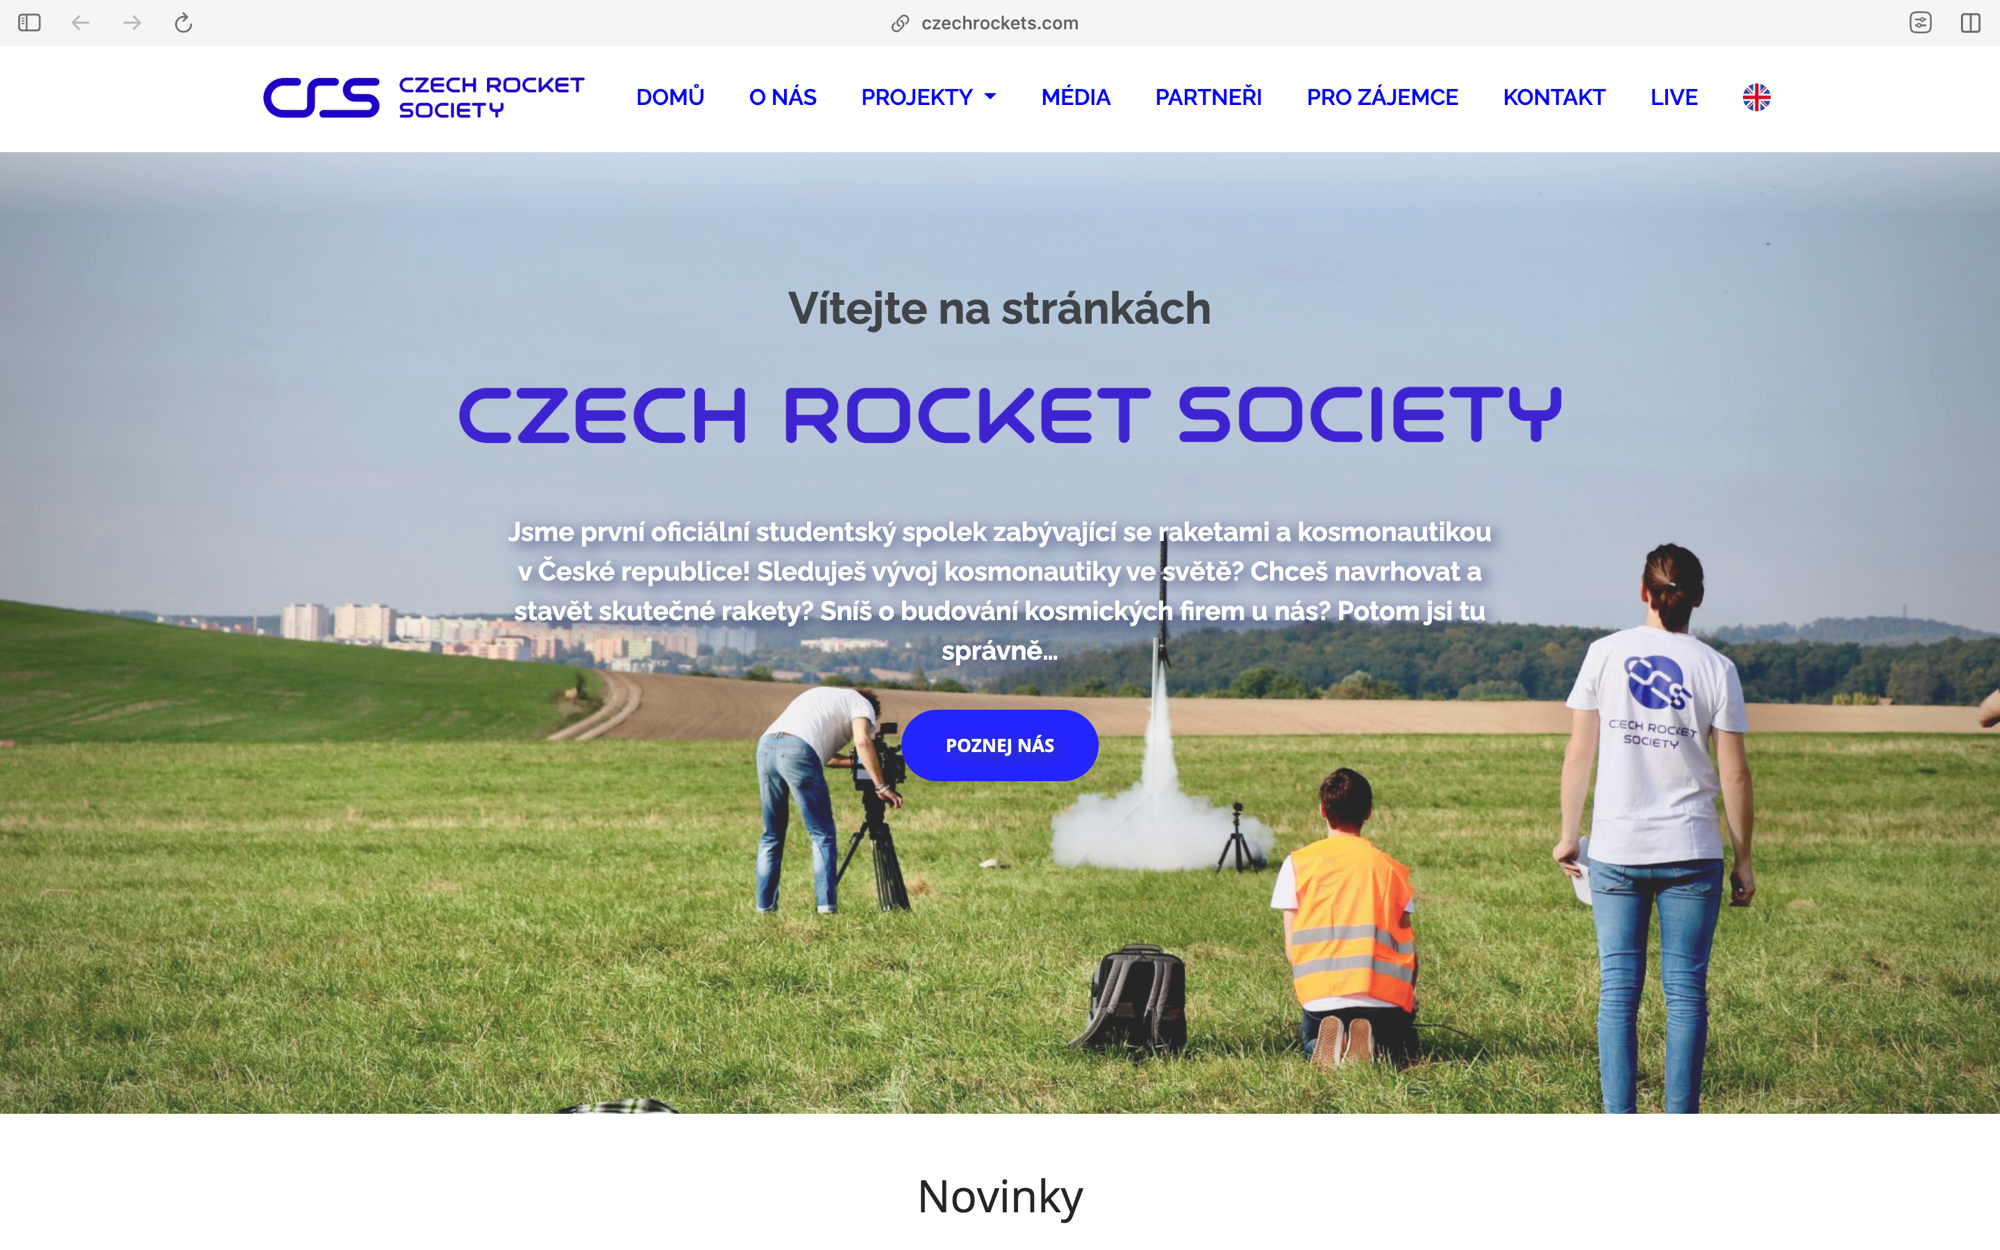
\includegraphics[width=\textwidth]{crs-current-web.png}
\caption{Úvodní stránka stávajícího webu Czech Rocket Society~\cite{crs2024web}.}
\label{fig:crs-current-web}
\end{figure}


\section{Webové technologie}

\subsection{Architektura webových aplikací}

\begin{sloppypar}
Moderní webové aplikace jsou typicky postaveny na~modelu \textbf{klient-server}, kde frontend komunikuje s~backendem prostřednictvím REST (Representational State Transfer) API~\cite{fielding2000rest}. Přístup \textbf{API-first} striktně odděluje obě části systému, což umožňuje jejich nezávislý vývoj, testování a~případnou integraci s~dalšími klienty.
\end{sloppypar}

Při návrhu webové aplikace je zásadní volba způsobu vykreslování. \textbf{SPA} (Single Page Application) přenáší vykreslování na klienta, což poskytuje plynulou interakci, ale zhoršuje úvodní načtení a~SEO. \textbf{SSR} (Server-Side Rendering) generuje HTML na serveru při každém požadavku, čímž zlepšuje výkon i~indexaci. \textbf{SSG} (Static Site Generation) generuje stránky při sestavení aplikace a~\textbf{ISR} (Incremental Static Regeneration) kombinuje SSG s~průběžnou aktualizací~\cite{verma2024ssr, jartarghar2022nextjs}.

\begin{sloppypar}
Pro projekty skládající se z~více souvisejících částí (frontend, backend, sdílené knihovny) se nabízí organizace do~\textbf{monorepo} -- jediného repozitáře obsahujícího všechny komponenty systému. Tento přístup, prověřený organizacemi jako Google~\cite{potvin2016monorepo}, přináší jednotnou správu závislostí a~atomické změny napříč celým systémem.
\end{sloppypar}

\subsection{Frontend -- React a~Next.js}

\textbf{React} je knihovna pro tvorbu uživatelských rozhraní vyvíjená společností Meta a~open-source komunitou~\cite{react2024docs, elrom2021react}. Rozhraní je deklarativně složeno ze~znovupoužitelných komponent, které spravují vlastní stav. React efektivně aktualizuje DOM prostřednictvím \textbf{virtuálního DOM} (Document Object Model) -- při změně stavu porovná nový virtuální strom s~předchozím a~aplikuje pouze minimální změny.

\textbf{Next.js} rozšiřuje React o~serverové vykreslování a~pokročilé routování~\cite{nextjs2024docs}. V~architektuře App Router zavádí koncept \textbf{serverových komponent}, které se vykreslují na serveru bez odesílání JavaScriptu klientovi, a~\textbf{klientských komponent} pro interaktivní části rozhraní~\cite{pati2025nextjs}. Díky tomu je vhodný pro aplikace kombinující veřejný obsah (SSR pro SEO) s~administračním rozhraním (SPA)~\cite{thakkar2020ssr}.

\subsection{Backend -- Node.js a~Hono}

\textbf{Node.js} je běhové prostředí pro JavaScript s~událostmi řízenou architekturou a~neblokujícím I/O (Input/Output)~\cite{tilkov2010nodejs}. Hlavní smyčka událostí (event loop) běží v~jediném vlákně, zatímco blokující vstupně-výstupní operace jsou delegovány na~pracovní thread pool knihovny libuv a~po~dokončení je zavolána funkce zpětného volání~\cite{nodejs2024eventloop}. Díky tomu Node.js efektivně zvládá velké množství souběžných připojení.

\begin{sloppypar}
\textbf{Hono}\footnote{\url{https://hono.dev/}} je lehký webový framework navržený pro TypeScript a~webové standardy~\cite{hono2024docs}. Hono využívá Web Standard API (Request, Response), díky čemuž není vázán na~konkrétní běhové prostředí. Framework používá middleware pattern a~oproti Express nabízí nativní podporu TypeScriptu a~integraci s~validační knihovnou Zod~\cite{hono2024github}.
\end{sloppypar}

\subsection{TypeScript}

\textbf{TypeScript} je nadmnožina JavaScriptu se statickým typovým systémem~\cite{typescript2024docs}. Typy jsou kontrolovány při kompilaci a~výstupem je čistý JavaScript. Statické typování prokazatelně snižuje počet chyb v~kódu ještě před nasazením~\cite{gao2017typescript}. V~monorepo architektuře TypeScript umožňuje definovat datové struktury konzistentně napříč celým systémem a~snižuje tak riziko nekonzistence mezi frontendem a~backendem. Pro validaci vstupních dat na straně API je použita knihovna \textbf{Zod}, která z~validačního schématu automaticky odvozuje TypeScriptový typ -- schéma tak slouží jako jediný zdroj pravdy pro strukturu i~validaci přijímaných dat.

\subsection{Go jako jazyk pro výkonnostně kritické služby}

\textbf{Go} je kompilovaný jazyk od Googlu, který produkuje jediný binární soubor bez externích závislostí~\cite{donovan2015go}. Hlavní předností je nativní podpora \textbf{konkurenčního programování} prostřednictvím goroutin -- lehkých vláken spotřebovávajících řádově kilobajty paměti -- a~kanálů pro bezpečnou komunikaci mezi nimi~\cite{tu2019go, gospec2024}. Tento model je vhodný pro služby zpracovávající vysokofrekvenční datové toky, kde je vyžadována nízká latence -- například při příjmu telemetrických dat, jejich perzistenci a~současné distribuci klientům.

Pro zpracování vysokofrekvenčních telemetrických dat je výhodný předvídatelný paměťový model a~lehká konkurenční primitiva, díky kterým lze snadno paralelizovat příjem, perzistenci a~distribuci dat bez složité synchronizace.

\section{Databázové systémy}

\subsection{Relační databáze -- PostgreSQL}

Relační databáze ukládají data do~tabulek propojených definovanými vztahy. Tento model, formálně popsaný Coddem~\cite{codd1970relational}, zajišťuje konzistenci dat prostřednictvím vlastností ACID (Atomicity, Consistency, Isolation, Durability) a~umožňuje jejich efektivní dotazování jazykem~SQL.

\textbf{PostgreSQL} je objektově-relační databázový systém, jehož počátky sahají k~projektu POSTGRES na UC Berkeley~\cite{stonebraker1986postgres}. Oproti alternativám jako MySQL nebo SQLite nabízí PostgreSQL pokročilé datové typy (JSONB -- JSON Binary, UUID -- Universally Unique Identifier, vlastní výčtové typy), silnou podporu standardu SQL a~prověřenou škálovatelnost~\cite{postgresql2024docs}. Kombinace relačního modelu s~možností ukládat polostrukturovaná data v~JSONB sloupcích je výhodná pro aplikace, kde většina entit má pevnou strukturu, ale některé atributy vyžadují flexibilitu.

\subsection{Časové databáze -- InfluxDB}

Telemetrická data z~raketových letů mají charakter \textbf{časových řad} -- sekvencí měření indexovaných časovým razítkem, kde nová data neustále přibývají a~u~starších záznamů roste význam agregovaných trendů oproti jednotlivým vzorkům~\cite{kaknjo2019lowcost}. Relační databáze nejsou pro tento typ zátěže optimalizovány, protože standardní B-tree indexy a~řádkové úložiště nedosahují potřebného výkonu při vysoké frekvenci zápisů~\cite{grzesik2020tsdb}.

\textbf{InfluxDB} je specializovaná časová databáze navržená pro vysoký průchod zápisů a~efektivní agregační dotazy nad časovými rozsahy~\cite{influxdb2024docs}. Využívá vlastní úložný engine TSM (Time-Structured Merge Tree) optimalizovaný pro sekvenční zápis a~nabízí vestavěné mechanismy jako retenční politiky pro automatický životní cyklus dat a~dávkový zápis pro minimalizaci I/O operací. Pro systémy zpracovávající vysokofrekvenční senzorová data s~požadavkem na nízkou latenci zápisu představuje časová databáze vhodnější volbu než ukládání časových řad do relační databáze.

\subsection{ORM -- Drizzle}

\textbf{Object-Relational Mapping} (ORM) je technika, která mapuje objekty programovacího jazyka na tabulky relační databáze a~odstraňuje tak nutnost psát SQL dotazy ručně~\cite{torres2017orm}. Hlavní výhodou je zvýšení produktivity a~snížení rizika chyb při zachování typové bezpečnosti, nevýhodou může být ztráta kontroly nad generovanými dotazy.

\textbf{Drizzle ORM} volí přístup schema-as-code -- databázové schéma je definováno přímo v~TypeScriptu, z~čehož se automaticky odvozují jak typové definice, tak databázové migrace~\cite{drizzle2024docs}. Oproti alternativám jako Prisma, která používá vlastní definiční jazyk, Drizzle zůstává blízko~SQL syntaxi, což usnadňuje ladění dotazů a~snižuje abstrakční bariéru. Migrace jsou generovány jako čisté SQL soubory, které lze verzovat společně se~zdrojovým kódem.

\section{Autentizace a bezpečnost}

\subsection{JWT -- JSON Web Token}

Webová API postavená na~principu REST jsou ze~své podstaty bezstavová -- server neuchovává informaci o~přihlášeném uživateli mezi jednotlivými požadavky~\cite{fielding2000rest}. Pro autentizaci je proto potřeba mechanismus, který umožní ověřit identitu uživatele bez nutnosti uchovávat stav sezení na~serveru.

\textbf{JSON Web Token} (JWT) je otevřený standard definovaný v~RFC (Request for Comments)~7519~\cite{rfc7519jwt}. Token se skládá ze~tří částí: hlavičky s~algoritmem podpisu, datové části -- tzv. payload (datový obsah zprávy) -- s~tvrzeními o~uživateli (identifikátor, role, doba expirace) a~digitálního podpisu. Podpis je vytvořen kódem HMAC (Hash-based Message Authentication Code), který kombinuje hlavičku a~payload s~tajným klíčem uloženým na~serveru, a~je počítán prostřednictvím hashovací funkce (typicky SHA-256). Standard podporuje i~asymetrické algoritmy podpisu (RSA, ECDSA), jejichž volba je signalizována v~hlavičce tokenu. Při ověření server stejným způsobem spočítá podpis znovu a~porovná jej s~podpisem v~tokenu, čímž ověří, že obsah nebyl pozměněn, aniž by potřeboval dotazovat databázi nebo uchovávat stav sezení. To je pro API-first architekturu výhodnější než klasické serverové sessions vyžadující sdílené úložiště. Nevýhodou je, že vydaný token nelze jednoduše revokovat před vypršením jeho platnosti. Je proto nutné dodržovat bezpečnostní doporučení -- zejména ověřování algoritmu podpisu, nastavení krátké expirace a~přenos výhradně přes HTTPS (Hypertext Transfer Protocol Secure)~\cite{rfc8725jwt}.

\subsection{Hashování hesel}

Hesla uživatelů nesmí být ukládána v~čitelné podobě ani šifrována reverzibilním algoritmem -- v~případě úniku databáze by bylo možné je rekonstruovat. Místo toho se používá jednosměrné \textbf{hashování}, při kterém z~hesla vznikne otisk fixní délky, ze kterého nelze zpětně odvodit původní vstup~\cite{owasp2024password}.

Mezi osvědčené hashovací algoritmy patří \textbf{bcrypt}, navržený Provosem a~Mazièresem specificky pro ukládání hesel~\cite{provos1999bcrypt}. Klíčovou vlastností bcryptu je nastavitelná výpočetní náročnost (cost factor) -- s~rostoucím výkonem hardwaru lze náročnost zvýšit, čímž se zachovává odolnost proti útokům hrubou silou. Ke~každému heslu se automaticky generuje náhodná sůl, která zabraňuje použití předpočítaných tabulek~\cite{owasp2024password}. Současná doporučení OWASP uvádějí jako primární volbu pro nově vyvíjené aplikace algoritmus Argon2id, bcrypt však zůstává široce používán pro svou stabilitu a~dostupnost knihoven.

\subsection{RBAC -- řízení přístupu na~základě rolí}

\textbf{Role-Based Access Control} (RBAC) je model řízení přístupu, ve kterém jsou oprávnění přiřazena rolím a~uživatelům jsou přiděleny odpovídající role~\cite{sandhu1996rbac}. Oproti individuálnímu přidělování oprávnění každému uživateli tento přístup zjednodušuje administraci a~snižuje riziko chybné konfigurace. V~jednodušších aplikacích pro správu obsahu typicky postačují dvě role -- administrátor s~plným přístupem ke správě systému a~editor s~oprávněním vytvářet a~upravovat obsah.

\section{Real-time komunikace}

\subsection{MQTT protokol}

\textbf{MQTT} (Message Queuing Telemetry Transport) je lehký messaging protokol založený na vzoru \textbf{publish/subscribe}, standardizovaný organizací OASIS~\cite{mqtt2014oasis}. Protokol byl navržen pro nespolehlivé sítě s~omezenou šířkou pásma a~nízkovýkonná zařízení, což jej činí vhodným pro aplikace v~oblasti internetu věcí (IoT) a~telemetrie~\cite{mishra2020mqtt}.

Komunikace v~MQTT probíhá prostřednictvím centrálního \textbf{brokeru}, který zprostředkovává výměnu zpráv mezi producenty (publishers) a~konzumenty (subscribers). Producent odesílá zprávy na pojmenovaný \textbf{topic} (téma), broker je přijme a~doručí všem klientům, kteří se k~danému tématu přihlásili. Klienti se tak nemusí vzájemně znát ani být současně připojeni -- broker zajišťuje oddělení v~čase i~prostoru~\cite{quincozes2019mqtt}.

Protokol definuje tři úrovně kvality doručení (\textbf{QoS}), které umožňují přizpůsobit spolehlivost přenosu požadavkům aplikace~\cite{mqtt2014oasis}. Pro telemetrická data, kde je důležitější nízká latence než garance doručení každého vzorku, se typicky volí nejnižší úroveň~\cite{kegenbekov2022mqtt}.

\begin{sloppypar}
Mezi nejrozšířenější open-source implementace MQTT brokeru patří \textbf{Mosquitto}~\cite{light2017mosquitto}.
\end{sloppypar}

\subsection{WebSocket}

\begin{sloppypar}
\textbf{WebSocket} je komunikační protokol definovaný v~RFC~6455, který umožňuje \textbf{obousměrnou} (full-duplex) komunikaci mezi klientem a~serverem přes jediné TCP (Transmission Control Protocol) spojení~\cite{rfc6455websocket}. Na~rozdíl od~tradičního HTTP, kde klient musí opakovaně posílat požadavky (polling) pro zjištění nových dat, WebSocket umožňuje serveru aktivně zasílat data klientovi v~okamžiku jejich vzniku (push model).
\end{sloppypar}

Spojení se navazuje prostřednictvím \textbf{HTTP Upgrade handshake} -- klient odešle standardní HTTP požadavek s~hlavičkou \texttt{Upgrade: websocket} a~po úspěšné odpovědi serveru (stavový kód 101) se spojení přepne na WebSocket protokol~\cite{rfc6455websocket}. Od tohoto okamžiku mohou obě strany nezávisle odesílat zprávy ve formě rámců (frames), které obsahují minimální režijní hlavičku o~velikosti 2--14~bajtů.

Alternativou k~WebSocket je technologie \textbf{Server-Sent Events} (SSE), která rovněž umožňuje push komunikaci, avšak pouze jednosměrně -- od serveru ke klientovi. SSE využívá standardní HTTP spojení a~je jednodušší na implementaci, ale neumožňuje obousměrnou výměnu dat. Pro aplikace vyžadující interaktivní komunikaci v~reálném čase, jako je živé zobrazení telemetrie s~možností řízení odběru dat, představuje WebSocket vhodnější řešení~\cite{murley2021websocket}.

\section{Kontejnerizace}

\subsection{Docker}

\textbf{Docker} je platforma pro kontejnerizaci aplikací, která umožňuje zabalit software spolu se všemi jeho závislostmi do izolované jednotky zvané \textbf{kontejner}~\cite{sipek2018docker}. Kontejner sdílí jádro hostitelského operačního systému, ale má vlastní souborový systém, síťový prostor a~procesy. Díky tomu je spuštění kontejneru řádově rychlejší a~méně náročné na prostředky než spuštění virtuálního stroje, který vyžaduje kompletní operační systém včetně vlastního jádra.

\begin{sloppypar}
Kontejnery se vytvářejí z~\textbf{obrazů} (images), které jsou definovány souborem \texttt{Dockerfile}. Obraz je složen z~vrstev (layers), kde každá vrstva odpovídá jedné instrukci v~\texttt{Dockerfile} -- například instalaci závislostí nebo kopírování zdrojového kódu~\cite{docker2024overview}. Vrstvy jsou sdílené a~cachované, což zrychluje opakované sestavení. Hlavní výhodou kontejnerizace je konzistence prostředí -- aplikace běží stejně na~vývojářském počítači, v~testovacím prostředí i~v~produkci.
\end{sloppypar}

\subsection{Docker Compose}

\textbf{Docker Compose} je nástroj pro definici a~orchestraci vícekontejnerových aplikací pomocí jediného konfiguračního souboru ve formátu YAML (YAML Ain't Markup Language)~\cite{docker2024overview}. V~tomto souboru se deklarativně popisují jednotlivé služby, jejich obrazy, síťové propojení, proměnné prostředí a~datové svazky (volumes).

Compose automaticky vytváří společnou síť pro všechny definované služby, ve které se kontejnery vzájemně adresují svými názvy jako hostitelskými jmény. Dále umožňuje definovat závislosti mezi službami a~podmínky spuštění -- například požadavek, aby databáze hlásila zdravý stav dříve, než se spustí aplikační server. Pro projekty menšího a~středního rozsahu představuje Docker Compose dostatečné řešení, které nevyžaduje komplexní orchestrátory jako Kubernetes.

\section{Testování webových aplikací}

Testování je nedílnou součástí vývoje software, jehož cílem je ověřit, že systém splňuje specifikované požadavky a~funguje správně za různých podmínek~\cite{sommerville2016se}. U~webových aplikací, kde spolu interaguje frontend, backend, databáze a~externí služby, je testování obzvlášť důležité kvůli množství integračních bodů, které mohou být zdrojem chyb.

\subsection{Úrovně testování}

Testování software se tradičně dělí do několika úrovní podle rozsahu testované jednotky~\cite{sommerville2016se}. Tento koncept je často vizualizován jako \textbf{testovací pyramida}, kterou poprvé popsal Cohn~\cite{cohn2010agile} -- na základně stojí velké množství rychlých unit testů, nad nimi menší počet integračních testů a~na vrcholu malý počet end-to-end testů.

\textbf{Unit testy} (jednotkové testy) ověřují správnost izolovaných jednotek kódu -- typicky funkcí, metod nebo modulů -- nezávisle na zbytku systému~\cite{beck2003tdd}. Závislosti testované jednotky se nahrazují testovacími dvojníky (mocks, stubs), čímž se zajišťuje, že test selhává pouze kvůli chybě v~testovaném kódu, nikoli kvůli chybě v~závislosti~\cite{meszaros2007xunit}. Unit testy jsou nejrychlejší a~nejlevnější na údržbu, proto by jich mělo být nejvíce.

\textbf{Integrační testy} ověřují spolupráci mezi dvěma a~více komponentami systému -- například zda API endpoint správně zpracuje HTTP požadavek, provede validaci, zavolá databázi a~vrátí očekávanou odpověď~\cite{sommerville2016se}. Na rozdíl od unit testů, které testují komponenty izolovaně, integrační testy odhalují chyby ve vzájemné komunikaci komponent.

\textbf{Manuální (explorativní) testování} doplňuje automatizované testy v~oblastech, kde je automatizace náročná nebo neefektivní -- zejména při ověřování vizuální správnosti uživatelského rozhraní, uživatelské přívětivosti a~komplexních interaktivních scénářů~\cite{whittaker2009exploratory}. Tester při explorativním testování aktivně prozkoumává aplikaci bez předem definovaného skriptu a~využívá své zkušenosti k~odhalování neočekávaného chování.

\subsection{Jest jako testovací framework}

\textbf{Jest}\footnote{\url{https://jestjs.io/}} je testovací framework pro JavaScript a~TypeScript původně vyvinutý společností Meta, dnes spravovaný pod záštitou OpenJS Foundation~\cite{jest2024docs}. Jest poskytuje kompletní testovací prostředí zahrnující test runner, assertion knihovnu, mocking systém a~generování code coverage reportů v~jediném balíčku bez nutnosti konfigurace externích závislostí.

Pro TypeScript projekty se Jest typicky používá s~transpilerem \textbf{ts-jest}, který umožňuje spouštět testy přímo z~TypeScriptových souborů. Jest podporuje paralelní spouštění testů, automatické sledování změn souborů (watch mode) a~snapshot testování pro ověřování struktury výstupních dat.

\chapter{Návrh řešení}
\label{chap:navrh}

\section{Architektura aplikace}

Platforma je navržena jako soustava tří samostatných aplikací doplněných infrastrukturními službami. Aplikace \texttt{web} (Next.js) zajišťuje prezentační vrstvu, \texttt{api} (Hono) poskytuje REST rozhraní pro správu obsahu a~\texttt{telemetry} (Go) zpracovává telemetrická data v~reálném čase. Infrastrukturu tvoří relační databáze PostgreSQL, časová databáze InfluxDB a~MQTT broker Mosquitto. Celkový pohled na architekturu znázorňuje obrázek~\ref{fig:architecture}.

\begin{figure}[ht]
\centering
\begin{tikzpicture}[
    app/.style={rectangle, draw, rounded corners, minimum height=1.1cm, minimum width=3cm, align=center, font=\small, fill=blue!8},
    infra/.style={rectangle, draw, rounded corners, minimum height=1.1cm, minimum width=3cm, align=center, font=\small, fill=gray!15},
    ext/.style={rectangle, draw, rounded corners, dashed, minimum height=1.1cm, minimum width=3cm, align=center, font=\small},
    arr/.style={-{Stealth[length=3mm]}, thick},
    lbl/.style={font=\footnotesize, fill=white, inner sep=1.5pt}
]
    % Pozice — 3 sloupce: levý (0), střed (5), pravý (10)

    % Řádek 1 — externí
    \node[ext] (browser) at (0, 0) {Prohlížeč};
    \node[ext] (device) at (10, 0) {Raketa / Simulátor};

    % Řádek 2 — frontend + broker
    \node[app] (web) at (0, -2.5) {Next.js\\{\footnotesize (frontend)}};
    \node[infra] (mqtt) at (10, -2.5) {Mosquitto\\{\footnotesize (MQTT broker)}};

    % Řádek 3 — backend + Go server
    \node[app] (api) at (0, -5) {Hono API\\{\footnotesize (backend)}};
    \node[app] (telemetry) at (10, -5) {Go server\\{\footnotesize (telemetrie)}};

    % Řádek 4 — databáze + služby
    \node[infra] (postgres) at (-1, -7.5) {PostgreSQL};
    \node[infra] (mailhog) at (2.5, -7.5) {MailHog\\{\footnotesize (SMTP)}};
    \node[infra] (influx) at (10, -7.5) {InfluxDB};

    % === Vertikální šipky (hlavní toky) ===
    \draw[arr] (browser) -- node[lbl, left] {HTTP} (web);
    \draw[arr] (web) -- node[lbl, left] {REST API} (api);
    \draw[arr] (api) -- node[lbl, left] {SQL} (postgres);
    \draw[arr] (api) -- node[lbl, right] {SMTP} (mailhog);
    \draw[arr] (device) -- node[lbl, right] {MQTT publish} (mqtt);
    \draw[arr] (mqtt) -- node[lbl, right] {subscribe} (telemetry);
    \draw[arr] ($(telemetry.south)+(0.3,0)$) -- node[lbl, right] {write} ($(influx.north)+(0.3,0)$);
    \draw[arr] ($(influx.north)+(-0.3,0)$) -- node[lbl, left] {read} ($(telemetry.south)+(-0.3,0)$);

    % === Cross-stack šipky ===

    % WebSocket: Go server → Prohlížeč (horizontálně do středu, pak nahoru, pak do pravého boku prohlížeče)
    \draw[arr] (telemetry.west) -- node[lbl, above] {WebSocket} (browser.east);

    % MQTT-over-WS: Mosquitto → Prohlížeč (nahoru, pak vlevo do pravého horního rohu)
    \draw[arr, dashed] (mqtt.west) -- node[lbl, above] {\footnotesize MQTT-over-WS}  (browser.north east);

\end{tikzpicture}
\caption{Architektura platformy a~komunikační toky mezi komponentami.}
\label{fig:architecture}
\end{figure}

\subsection{Monorepo struktura}

Zdrojový kód je organizován v~monorepo repozitáři spravovaném nástrojem \textbf{pnpm workspaces}. Repozitář obsahuje tři aplikace v~adresáři \texttt{apps/} -- frontend (\texttt{web}), backend (\texttt{api}) a~telemetrický server (\texttt{telemetry}) -- a~sdílený adresář \texttt{packages/} pro případné společné knihovny.

Monorepo přístup umožňuje provádět atomické změny napříč frontendem i~backendem v~jediném commitu, sdílet TypeScript typy a~Zod validační schémata mezi aplikacemi a~spravovat závislosti z~jednoho místa. Podrobná adresářová struktura repozitáře je uvedena v~kapitole~\ref{chap:implementace}.

\subsection{Komunikace mezi komponentami}

\begin{sloppypar}Frontend komunikuje s~backendem prostřednictvím REST API ve formátu JSON. Na~straně serveru Next.js používá pro API volání interní Docker adresu (\texttt{http://\allowbreak api:3001}), zatímco prohlížeč přistupuje přes externě dostupnou adresu (ve~vývoji \texttt{http://\allowbreak localhost:\allowbreak 3001}, v~produkci adresa nasazeného API). Klientská strana využívá knihovnu React Query pro cachování a~automatickou invalidaci dat.\end{sloppypar}

Backend přistupuje k~PostgreSQL skrze Drizzle ORM, který generuje typově bezpečné SQL dotazy. Telemetrický server v~Go odebírá zprávy z~MQTT brokeru, zapisuje je dávkově do InfluxDB a~současně je distribuuje připojeným klientům přes WebSocket. Pro vizualizaci telemetrických dat v~prohlížeči se primárně používá přímé připojení k~Mosquitto přes MQTT-over-WebSocket, které nevyžaduje běžící Go server a~poskytuje nejkratší cestu dat k~uživateli. Go server slouží jako alternativní kanál s~optimalizací distribuce dat.

\subsection{Kontejnerizace a vývojové prostředí}

\begin{sloppypar}
Vývojové prostředí je definováno pomocí Docker Compose, který orchestruje osm služeb platformy -- databáze (PostgreSQL, InfluxDB), komunikační služby (Mosquitto, MailHog), administrační nástroje (pgAdmin) a~aplikace (API, web, telemetrie). Všechny kontejnery sdílejí společnou síť a~vzájemně se adresují svými názvy služeb.
\end{sloppypar}

\section{Datový model}

Platforma využívá dva typy datových úložišť, z~nichž každé je optimalizováno pro odlišný charakter dat. Relační databáze PostgreSQL slouží k~ukládání strukturovaných dat systému správy obsahu -- uživatelských účtů, článků, událostí, projektů, členů, partnerů a~náborových přihlášek. Časová databáze InfluxDB je určena výhradně pro telemetrická data z~raketových letů, která mají charakter časových řad s~vysokou frekvencí zápisů.

Oddělení obou úložišť vychází z~odlišných požadavků na zápis a~dotazování. CMS data vyžadují transakční konzistenci (ACID), komplexní dotazy s~filtry a~relace mezi entitami. Telemetrická data naopak vyžadují vysoký průchod zápisů a~efektivní agregace nad časovými rozsahy.

\subsection{Relační schéma (PostgreSQL)}

Databázové schéma obsahuje devět tabulek pokrývajících všechny doménové entity platformy (kompletní ER diagram je uveden v~příloze~\ref{app:er-diagram}). Schéma je definováno přístupem schema-as-code v~TypeScriptu pomocí Drizzle ORM, z~čehož se automaticky generují migrace i~typové definice.

\paragraph{Přehled tabulek}

\begin{itemize}
    \item \textbf{users} -- administrátorské účty pro CMS (email, heslo, role \texttt{admin}/\texttt{editor})
    \item \textbf{articles} -- aktuality a~blogové příspěvky s~podporou kategorií, štítků a~rich-text obsahu
    \item \textbf{events} -- události spolku s~datem, místem a~typem (start, test, nábor, PR akce)
    \item \textbf{members} -- členové spolku s~kontaktními údaji, rolí, odborem a~profilovým obrázkem
    \item \textbf{projects} -- raketové projekty s~kategorií, technickými specifikacemi a~galerií
    \item \textbf{project\_members} -- vazební tabulka pro vztah M:N mezi projekty a~členy
    \item \textbf{recruitment\_submissions} -- náborové přihlášky s~kompletním workflow:\newline
    \texttt{draft} $\rightarrow$ \texttt{pending} $\rightarrow$ \texttt{interview\_scheduled} $\rightarrow$ \texttt{interviewed} $\rightarrow$ \texttt{accepted} $\rightarrow$ \texttt{documents\_sent} $\rightarrow$ \texttt{completed}\,/\,\texttt{rejected}
    \item \textbf{recruitment\_settings} -- konfigurace náborového procesu (dostupné role, úkoly)
    \item \textbf{partners} -- partnerské organizace s~třístupňovým systémem (silver, gold, diamond)
\end{itemize}

\paragraph{Návrhové volby}

\textbf{UUID primární klíče.} Všechny tabulky používají jako primární klíč UUID generovaný databází (\texttt{gen\_random\_uuid()}). Oproti sekvenčním identifikátorům UUID eliminuje riziko kolizí při distribuovaném zápisu a~neprozrazuje pořadí ani počet záznamů v~adresách URL (Uniform Resource Locator).

\textbf{JSONB sloupce pro flexibilní metadata.} Některé atributy entity nemají pevnou strukturu a~mohou se v~čase měnit. Pro tyto případy schéma využívá datový typ JSONB, který umožňuje ukládat polostrukturovaná data přímo v~relační tabulce. Konkrétně se jedná o~štítky článků a~členů (\texttt{tags}), galerie obrázků (\texttt{images}), technické specifikace projektů (\texttt{specs}) a~konfiguraci náborových rolí a~úkolů (\texttt{roles}, \texttt{tasks} v~tabulce \texttt{recruitment\_settings}).

\textbf{TEXT místo VARCHAR pro volné textové vstupy.} Sloupce přijímající uživatelský text (motivace, zkušenosti, poznámky administrátora) používají typ \texttt{TEXT} bez omezení délky. Pevné limity \texttt{VARCHAR} neumožňovaly dostatečnou flexibilitu při zadávání odpovědí v~náborovém formuláři, kde délka textu závisí na konkrétním uchazeči a~nelze ji předem odhadnout.

\begin{sloppypar} 
\textbf{Řízení viditelnosti obsahu.} Entity publikovatelné na~veřejném webu (články, události, projekty, partneři) kombinují dva mechanismy: booleovský příznak \texttt{published} pro jednoduché přepínání viditelnosti a~textový sloupec \texttt{status} pro detailnější workflow. Články používají stavy \texttt{draft}\,/\,\texttt{published}\,/\,\texttt{archived} a~projekty \texttt{planning}\,/\,\allowbreak\texttt{development}\,/\,\texttt{testing}\,/\,\texttt{completed}. Události nemají explicitní sloupec statusu -- jejich stav se automaticky odvozuje z~dat začátku a~konce, s~možností ručně nastavit speciální status \texttt{cancelled} nebo \texttt{pos\-tponed}.
\end{sloppypar}
\begin{sloppypar}
\textbf{Vlastní výčtový typ.} Pro partnerské úrovně je definován PostgreSQL enum \texttt{partner\-\_tier} s~hodnotami \texttt{silver}, \texttt{gold} a~\texttt{diamond}. Každá úroveň určuje rozsah zobrazovaných informací na~webu -- od~loga (silver) přes popis (gold) až po plnou prezentaci s~hero obrázkem (diamond).
\end{sloppypar}

\paragraph{Relace}

Schéma obsahuje dva typy relací. Vztah 1:N propojuje články s~autory -- sloupec \texttt{articles.author\_id} odkazuje na \texttt{users.id}. Vztah M:N mezi projekty a~členy je realizován prostřednictvím vazební tabulky \texttt{project\_members}, která navíc uchovává roli člena v~projektu (vedoucí, inženýr apod.). Obě reference ve vazební tabulce definují kaskádové mazání (\texttt{ON DELETE CASCADE}), aby odstranění projektu nebo člena automaticky vyčistilo přiřazení.

Všechny tabulky obsahují sloupce \texttt{created\_at} a~\texttt{updated\_at} s~výchozí hodnotou aktuálního časového razítka, které zajišťují auditní stopu pro každý záznam.

\subsection{Časové schéma (InfluxDB)}

InfluxDB organizuje data do tříúrovňové hierarchie: \textbf{organizace} (pracovní prostor sdružující uživatele a~přístupové tokeny), \textbf{bucket} (úložiště dat, obdoba databáze v~relačním modelu) a~\textbf{measurement} (obdoba tabulky, sdružuje datové body stejného typu). Telemetrická data platformy jsou ukládána v~bucketu \texttt{telemetry} v~rámci organizace \texttt{czech-rocket-society}, přičemž veškerá data sdílejí jediný measurement pojmenovaný \texttt{telemetry}.

\paragraph{Struktura záznamu}

Každý datový bod obsahuje čtyři tagy (indexované atributy pro efektivní filtrování) a~dynamickou sadu polí (měřené hodnoty):

\begin{sloppypar}
\begin{itemize}
    \item \textbf{Tagy:} \texttt{session\-\_id} (identifikátor letu nebo testu), \texttt{device\-\_type} (\texttt{rocket} nebo \texttt{test-stand}), \texttt{device\-\_id} (konkrétní zařízení) a~\texttt{data\-\_type} (kategorie dat -- \texttt{position}, \texttt{velocity}, \texttt{sensors}).
    \item \textbf{Pole:} dynamicky odvozená z~MQTT payloadu -- například \texttt{alt} (výška), \texttt{lat}/\texttt{lon} (GPS souřadnice), \texttt{vx}/\texttt{vy}/\texttt{vz} (složky rychlosti), \texttt{temp} (teplota), \texttt{pressure} (tlak) nebo \texttt{battery} (stav baterie).
    \item \textbf{Časové razítko:} jako vlastní časové razítko datového bodu se používá čas příjmu zprávy serverem. Pokud payload obsahuje pole \texttt{ts} (milisekundy od~epochy), server jej uloží jako pomocné pole \texttt{device\_ts} a~automaticky dopočítá latenci přenosu jako rozdíl obou časů.
\end{itemize}
\end{sloppypar}

Dynamická struktura polí umožňuje přidávat nové typy senzorů bez nutnosti úprav schématu -- server zapíše jakékoli klíče obsažené v~JSON payloadu jako pole datového bodu.

Telemetrická data z~raketových letů jsou uchovávána trvale, protože objem dat z~jednotlivých letů je relativně malý. Pro práci s~historickými daty poskytuje telemetrický server REST API s~podporou exportu do formátu CSV (Comma-Separated Values) a~JSON.

\section{Návrh API}

Platforma poskytuje dvě nezávislá API rozhraní. REST API postavené na frameworku Hono obsluhuje správu obsahu (CRUD -- Create, Read, Update, Delete -- operace nad všemi entitami), autentizaci a~nahrávání souborů. Telemetrické API v~Go zajišťuje distribuci dat v~reálném čase přes WebSocket a~přístup k~historickým měřením. Obě API komunikují výhradně ve formátu JSON (JavaScript Object Notation), používají standardní HTTP metody (GET, POST, PUT, DELETE) a~vracejí odpovídající stavové kódy (200, 201, 400, 401, 403, 404, 500).

\subsection{REST API (Hono)}

\paragraph{Přehled endpointů}

REST API je organizováno do devíti skupin endpointů připojených na společný prefix \texttt{/api}. Tabulka~\ref{tab:api-endpoints} uvádí přehled hlavních endpointů s~jejich autorizačními požadavky.

\begin{table}[ht]
\centering
\small
\begin{tabular}{llll}
\hline
\textbf{Skupina} & \textbf{HTTP metody} & \textbf{Zápis vyžaduje JWT} & \textbf{Popis} \\
\hline
\texttt{/auth} & POST & ne (registrace ano) & přihlášení, registrace \\
\texttt{/articles} & GET, POST, PUT, DELETE & ano & články a~aktuality \\
\texttt{/events} & GET, POST, PUT, DELETE & ano & události spolku \\
\texttt{/projects} & GET, POST, PUT, DELETE & ano & raketové projekty \\
\texttt{/members} & GET, POST, PUT, DELETE & ano & členové spolku \\
\texttt{/partners} & GET, POST, PUT, DELETE & ano & partnerské organizace \\
\texttt{/recruitment} & GET, POST, PUT & částečně & náborové přihlášky \\
\texttt{/upload} & POST, GET, DELETE & ano & nahrávání souborů \\
\texttt{/media} & POST, GET, DELETE & ano & správa obrázků \\
\hline
\end{tabular}
\caption{Přehled skupin API endpointů a~jejich autorizačních úrovní.}
\label{tab:api-endpoints}
\end{table}

Endpointy pro čtení dat (GET) jsou u~obsahových entit veřejné, přičemž neautentizovaným uživatelům se vrací pouze publikovaný obsah. Autentizovaný uživatel vidí i~nepublikované záznamy, což umožňuje náhled rozpracovaného obsahu v~administraci. Operace zápisu (POST, PUT, DELETE) vyžadují platný JWT token.

Každá obsahová entita (články, události, projekty) podporuje vyhledávání podle slugu -- unikátního textového identifikátoru odvozeného z~názvu, který slouží jako součást veřejné URL adresy.

\paragraph{Autorizační úrovně}

Přístupové účty nejsou veřejně dostupné -- vytváří je výhradně hlavní administrátor a~uděluje je pouze členům spolku, kteří mají obsah spravovat. Každý přihlášený uživatel je tedy důvěryhodný člen spolku s~oprávněním upravovat obsah platformy. Díky tomu API pracuje se dvěma základními úrovněmi přístupu:

\begin{enumerate}
    \item \textbf{Veřejný} -- endpoint je přístupný bez autentizace. Slouží pro čtení publikovaného obsahu, přihlášení do administrace a~odeslání náborové přihlášky.
    \item \textbf{Autentizovaný (JWT)} -- middleware \texttt{auth\-Middleware} ověří platnost tokenu z~hlavičky \texttt{Authorization:\allowbreak{} Bearer\allowbreak{} <token>} a~extrahuje identitu uživatele. Tato úroveň chrání veškeré operace zápisu (vytváření, editace, mazání obsahu) a~zpřístupňuje nepublikované záznamy pro náhled v~administraci.
\end{enumerate}

Tento model je dostatečný pro organizaci velikosti spolku, kde počet uživatelů s~přístupem do administrace je řádově v~jednotkách a~jejich oprávnění se řídí vzájemnou důvěrou. V~případě budoucího růstu lze systém rozšířit o~granulární role (například editor bez práva mazat obsah) zavedením dalšího middleware v~řetězci.

\paragraph{Validace vstupů}

Vstupní data na~POST a~PUT endpointech jsou validována pomocí knihovny Zod. Pro každou entitu je definováno schéma popisující povinná a~volitelná pole, datové typy a~povolené hodnoty (například výčet stavů \texttt{draft}\allowbreak/\allowbreak\texttt{published}\allowbreak/\allowbreak\texttt{archived} u~článků nebo \texttt{silver}\allowbreak/\allowbreak\texttt{gold}\allowbreak/\allowbreak\texttt{diamond} u~partnerů). Validace probíhá jako middleware před samotným zpracováním požadavku -- při neplatných datech server vrátí stavový kód 400 s~popisem chyb.

\paragraph{Nahrávání souborů}
\label{sec:navrh-upload}

Soubory jsou přijímány jako \texttt{multipart/form-data}. Server validuje typ souboru (obrázky: JPEG, PNG, WebP, GIF; dokumenty: PDF, DOCX) a~maximální velikost (5~MB). Nahrané soubory jsou ukládány do adresáře \texttt{/uploads/} a~servírovány prostřednictvím statického middleware na cestě \texttt{/uploads/*}.

Jednou nahrané soubory zůstávají v~knihovně médií a~lze je opakovaně vkládat do různého obsahu -- například tentýž obrázek může sloužit jako náhled článku i~jako fotografie v~galerii projektu. Administrační rozhraní pro práci s~knihovnou médií je popsáno v~kapitole~\ref{chap:implementace}.

\subsection{Telemetrické API (Go)}

Telemetrický server poskytuje WebSocket endpoint pro streaming v~reálném čase a~čtyři REST endpointy pro přístup k~historickým datům.

\begin{table}[ht]
\centering
\small
\begin{tabular}{lll}
\hline
\textbf{Metoda} & \textbf{Cesta} & \textbf{Popis} \\
\hline
GET & \texttt{/ws/telemetry} & WebSocket -- stream telemetrie v~reálném čase \\
GET & \texttt{/api/sessions} & seznam telemetrických sessions \\
GET & \texttt{/api/sessions/\{id\}/devices} & zařízení v~dané session \\
GET & \texttt{/api/history} & historická data s~downsampling \\
GET & \texttt{/api/history/export} & export dat (JSON nebo CSV) \\
\hline
\end{tabular}
\caption{Endpointy telemetrického API.}
\label{tab:telemetry-endpoints}
\end{table}

Telemetrické API nevyžaduje autentizaci -- data z~letů jsou veřejná a~přístupná všem návštěvníkům webu. WebSocket endpoint přijímá parametr \texttt{session\_id}, na jehož základě server filtruje a~odesílá pouze data z~požadované session. Způsob, jakým se data do telemetrického serveru dostávají prostřednictvím MQTT protokolu, je podrobně popsán v~sekci~\ref{sec:navrh-telemetrie}.

\section{Návrh uživatelského rozhraní}

Uživatelské rozhraní se skládá ze dvou oddělených částí se zásadně odlišným charakterem. Veřejná část je určena návštěvníkům webu -- využívá serverové vykreslování (SSR) pro optimalizaci načítání a~indexaci vyhledávači a~klade důraz na vizuální prezentaci. Administrační rozhraní je klientská aplikace (SPA) přístupná pouze přihlášeným členům spolku, zaměřená na efektivní správu obsahu.

\subsection{Veřejná část}
\label{sec:navrh-verejne-stranky}

\begin{sloppypar}
Veřejný web obsahuje čtrnáct stránek pokrývajících všechny prezentační potřeby spolku. Struktura stránek a~jejich URL cesty v~češtině jsou shrnuty v~tabulce~\ref{tab:public-routes}.
\end{sloppypar}

\begin{table}[ht]
\centering
\footnotesize
\begin{tabular}{lll}
\hline
\textbf{URL cesta} & \textbf{Stránka} & \textbf{Obsah} \\
\hline
\texttt{/} & úvodní stránka & hero sekce, statistiky, projekty, aktuality \\
\texttt{/aktuality} & seznam článků & mřížka článků s~náhledy a~výtahy \\
\texttt{/aktuality/[slug]} & detail článku & plný text s~obrázky \\
\texttt{/udalosti} & seznam událostí & karty s~datem, místem a~typem \\
\texttt{/udalosti/[slug]} & detail události & popis, mapa, termín \\
\texttt{/projekty} & přehled projektů & zvýrazněné a~běžné projekty \\
\texttt{/projekty/[slug]} & detail projektu & specifikace, tým, galerie \\
\texttt{/clenove} & členové spolku & mřížka s~fotkou, rolí a~odkazy \\
\texttt{/partneri} & partneři & třístupňové zobrazení dle tier \\
\texttt{/o-nas} & o~spolku & mise, hodnoty, správní rada \\
\texttt{/nabor} & náborový formulář & vícekrokový formulář \\
\texttt{/telemetrie} & telemetrický hub & seznam sessions, vstup do live \\
\texttt{/telemetrie/live/[id]} & živá telemetrie & grafy a~mapa v~reálném čase \\
\texttt{/telemetrie/playback/[id]} & historie letu & statické grafy, volba rozlišení \\
\hline
\end{tabular}
\caption{Struktura veřejných stránek platformy.}
\label{tab:public-routes}
\end{table}

\begin{figure}[H]
\centering
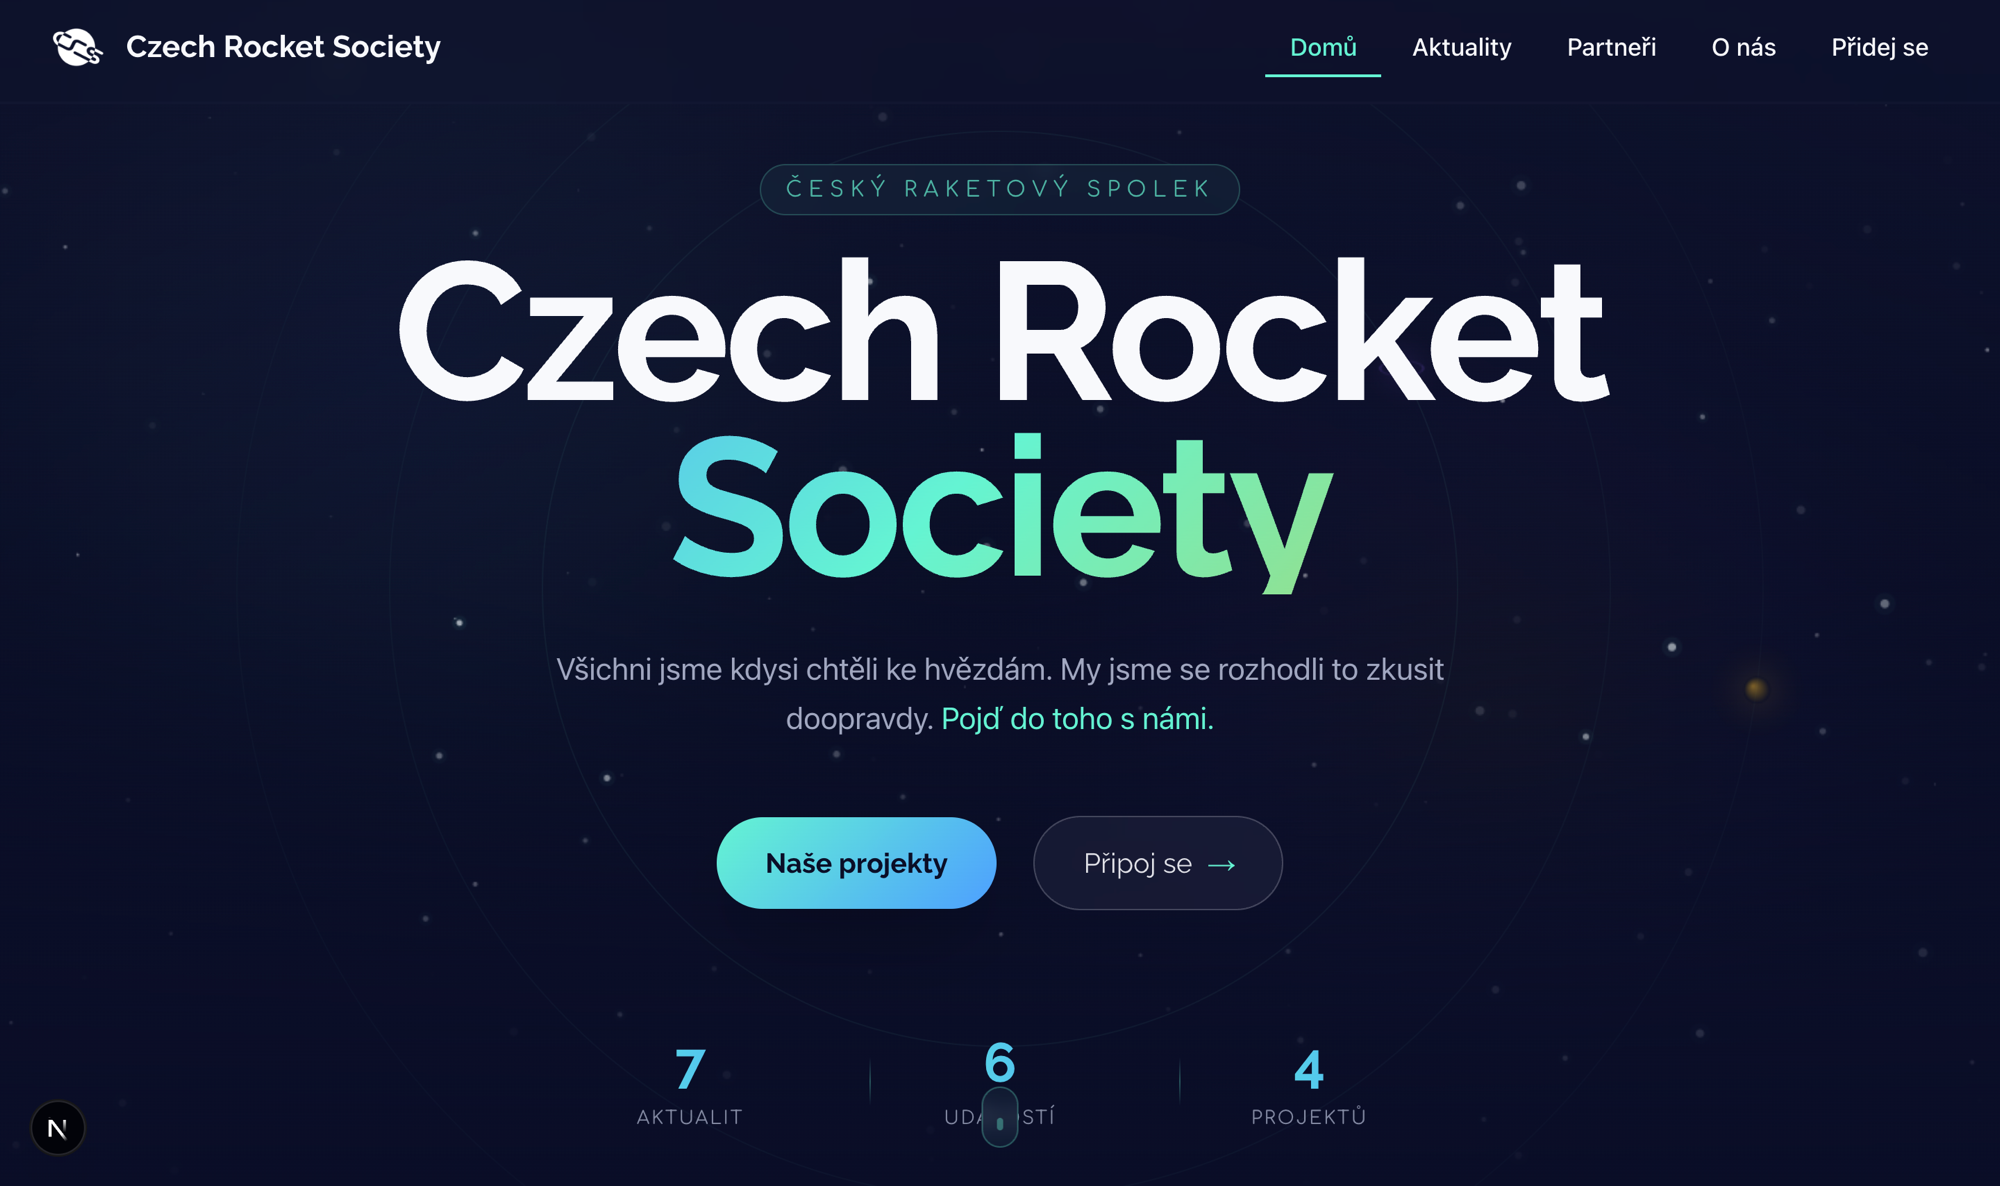
\includegraphics[width=\textwidth]{homepage.png}
\caption{Úvodní stránka veřejného webu Czech Rocket Society.}
\label{fig:homepage}
\end{figure}

Stránky s~dynamickým obsahem (články, události, projekty) používají v~URL adrese slug místo databázového identifikátoru. Slug je čitelný textový řetězec odvozený z~názvu entity (například \texttt{/aktuality/prvni-start-rakety-sherpa}), díky čemuž je adresa srozumitelná pro uživatele i~vyhledávače.

Všechny veřejné stránky jsou vykreslovány na~serveru (SSR) při každém požadavku, což zajišťuje, že návštěvník vždy obdrží aktuální obsah a~vyhledávače mohou stránky plně indexovat. Rozvržení je responzivní -- mřížky obsahu se přizpůsobují šířce obrazovky. Úvodní stránka veřejného webu je zachycena na~obrázku~\ref{fig:homepage}.

\subsection{Administrace}

Administrační rozhraní je přístupné na~cestě \texttt{/admin} a~chráněné middleware, který nepřihlášené uživatele přesměruje na~přihlašovací stránku. Po~přihlášení se zobrazí rozvržení se dvěma stálými prvky -- horní lištou s~informacemi o~přihlášeném uživateli a~tlačítkem pro odhlášení a~postranním menu s~navigací mezi sekcemi.

Administrace obsahuje následující sekce:
\begin{itemize}
    \item \textbf{Dashboard} -- přehled statistik (počty článků, událostí, členů, projektů) a~nedávno upravené záznamy s~rychlým přístupem k~editaci.
    \item \textbf{CRUD rozhraní} pro články, události, projekty, členy a~partnery -- každá entita má seznam záznamů s~možností filtrování, formulář pro vytvoření a~editaci. Články navíc disponují rich-text editorem pro formátování obsahu.
    \item \textbf{Správa náboru} -- seznam přijatých přihlášek s~filtrováním podle statusu, detail přihlášky s~vizualizací aktuálního workflow (viz sekce~\ref{sec:navrh-nabor-workflow}), možnost přidávat interní poznámky a~konfigurace dostupných rolí a~úkolů.
    \item \textbf{Knihovna médií} -- nahrávání obrázků, zobrazení galerie nahraných souborů a~jejich správa. Obrázky z~knihovny lze vkládat do~obsahu prostřednictvím modálního okna pro výběr.
    \item \textbf{Telemetrie} -- přístup k~telemetrickému dashboardu přímo z~administrace.
\end{itemize}

Ukázka administračního rozhraní pro správu událostí je zachycena na~obrázku~\ref{fig:admin-events}.

\begin{figure}[H]
\centering
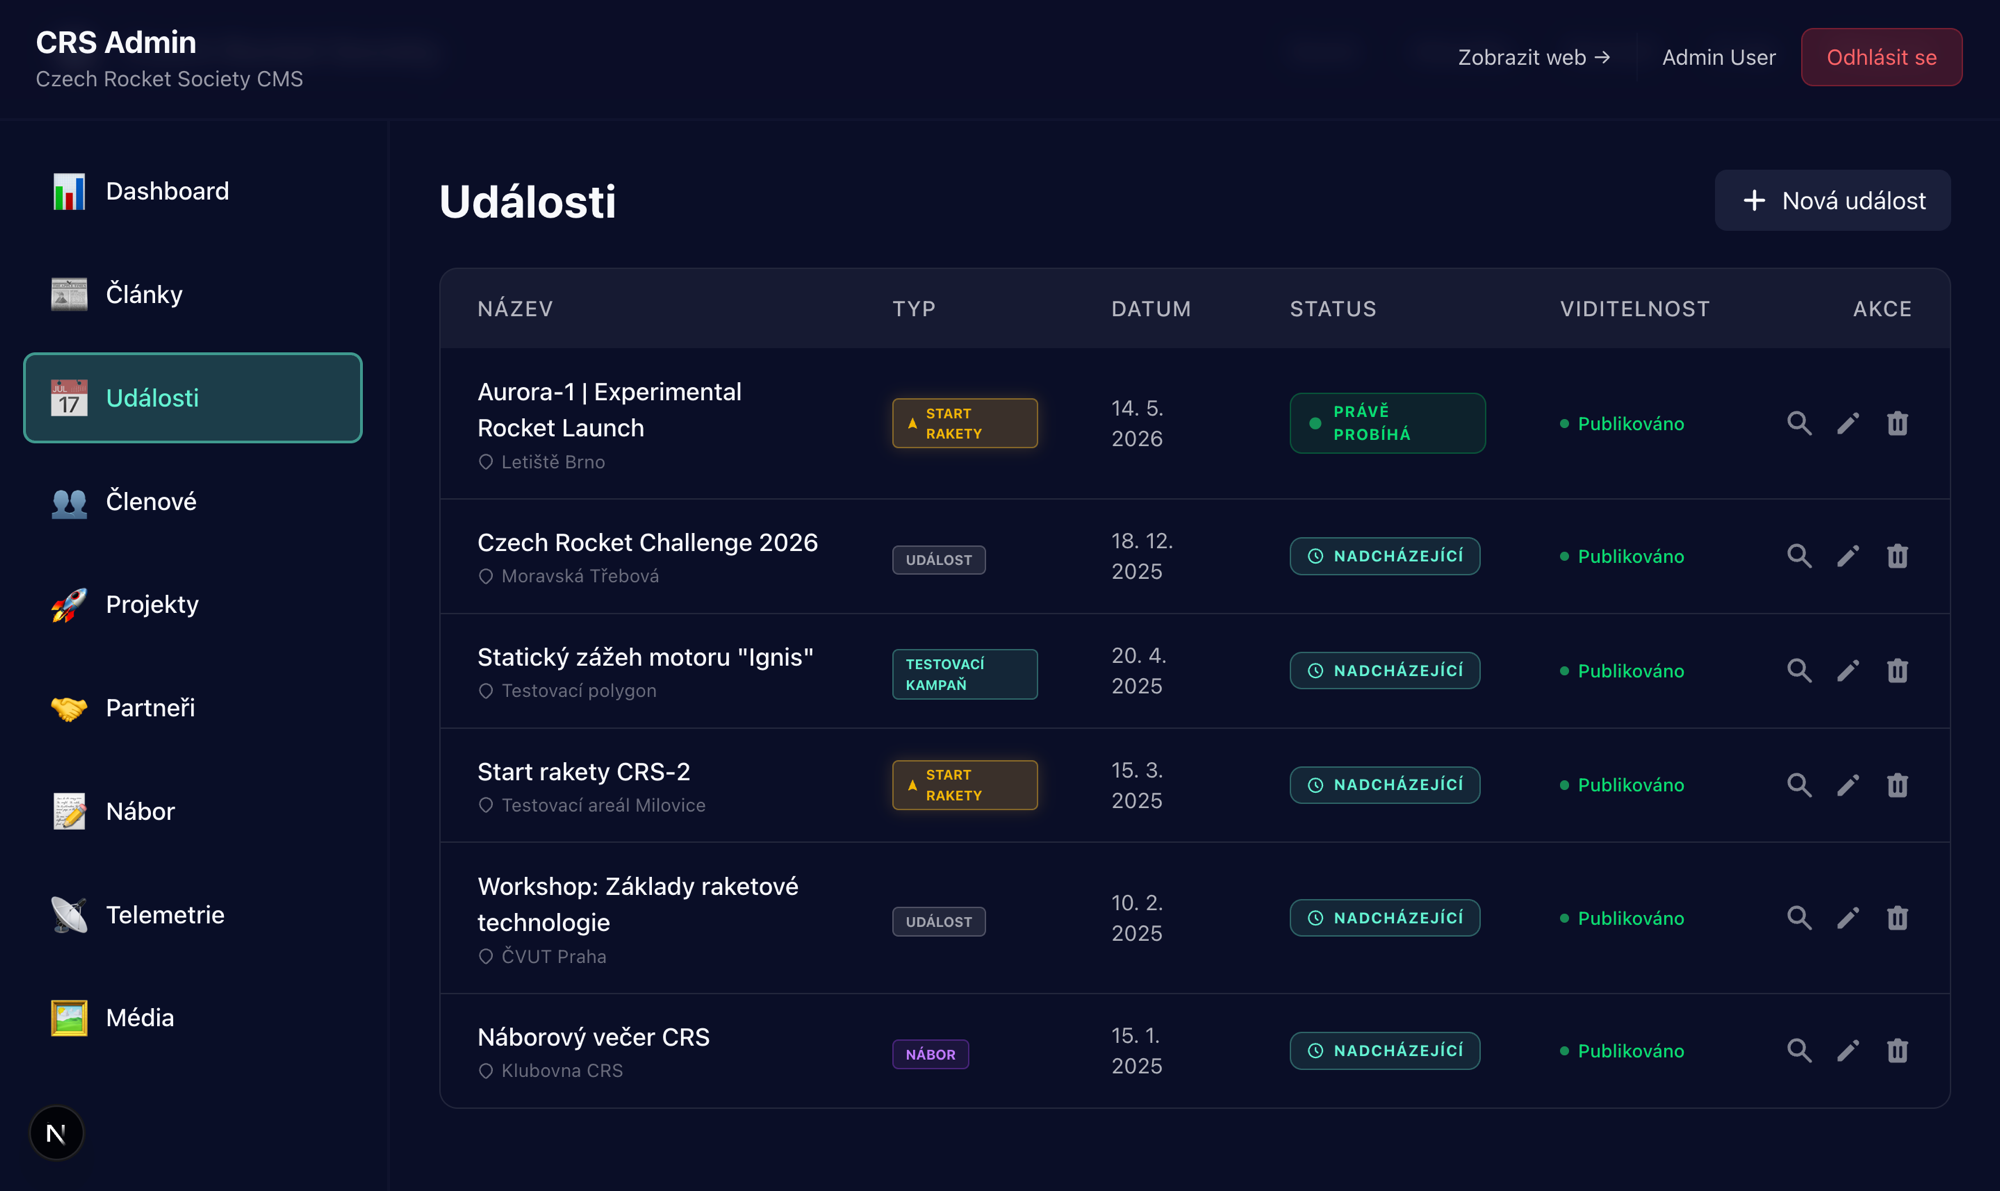
\includegraphics[width=\textwidth]{admin-events.png}
\caption{Administrační rozhraní -- správa událostí s~přehledem typů, statusů a~viditelnosti.}
\label{fig:admin-events}
\end{figure}

\section{Návrh náborového procesu}
\label{sec:navrh-nabor}

Náborový proces je navržen jako plně digitální workflow pokrývající cestu od prvního kontaktu zájemce až po jeho přijetí do spolku. Oproti stávajícímu řešení přes externí formulář na platformě JotForm přináší integrovaný formulář s~průběžným ukládáním, e-mailové notifikace a~administrační rozhraní pro správu přihlášek.

\subsection{Vícekrokový formulář}

Náborový formulář je rozdělen do šesti kroků, které uchazeče postupně provedou od zadání kontaktních údajů po odeslání kompletní přihlášky:

\begin{enumerate}
    \item \textbf{Základní údaje} -- jméno, e-mail a~telefonní číslo. Na základě e-mailu se vytvoří rozpracovaná přihláška (draft) a~uchazeči se odešle odkaz pro pokračování.
    \item \textbf{Zkušenosti} -- vzdělání, praxe a~technické dovednosti.
    \item \textbf{Motivace} -- proč se chce uchazeč připojit, oblasti zájmu, preferovaná role a~časová dostupnost.
    \item \textbf{Úloha} -- volitelná odpověď na úkol související se zvolenou oblastí zájmu.
    \item \textbf{Pohovor} -- rezervace termínu pohovoru prostřednictvím odkazu na plánovací nástroj.
    \item \textbf{Souhrn} -- přehled vyplněných dat s~možností vrátit se k~libovolnému kroku před odesláním.
\end{enumerate}

Každý krok validuje vstupní data samostatně -- uchazeč nemůže postoupit na~další krok bez vyplnění povinných polí. Povinná pole (motivace, jméno, vzdělání, zájmy) mají nastavené minimální délky, aby přihláška obsahovala dostatek informací pro posouzení. Ukázka jednoho z~kroků formuláře je zachycena na~obrázku~\ref{fig:recruitment-form}.

\begin{figure}[H]
\centering
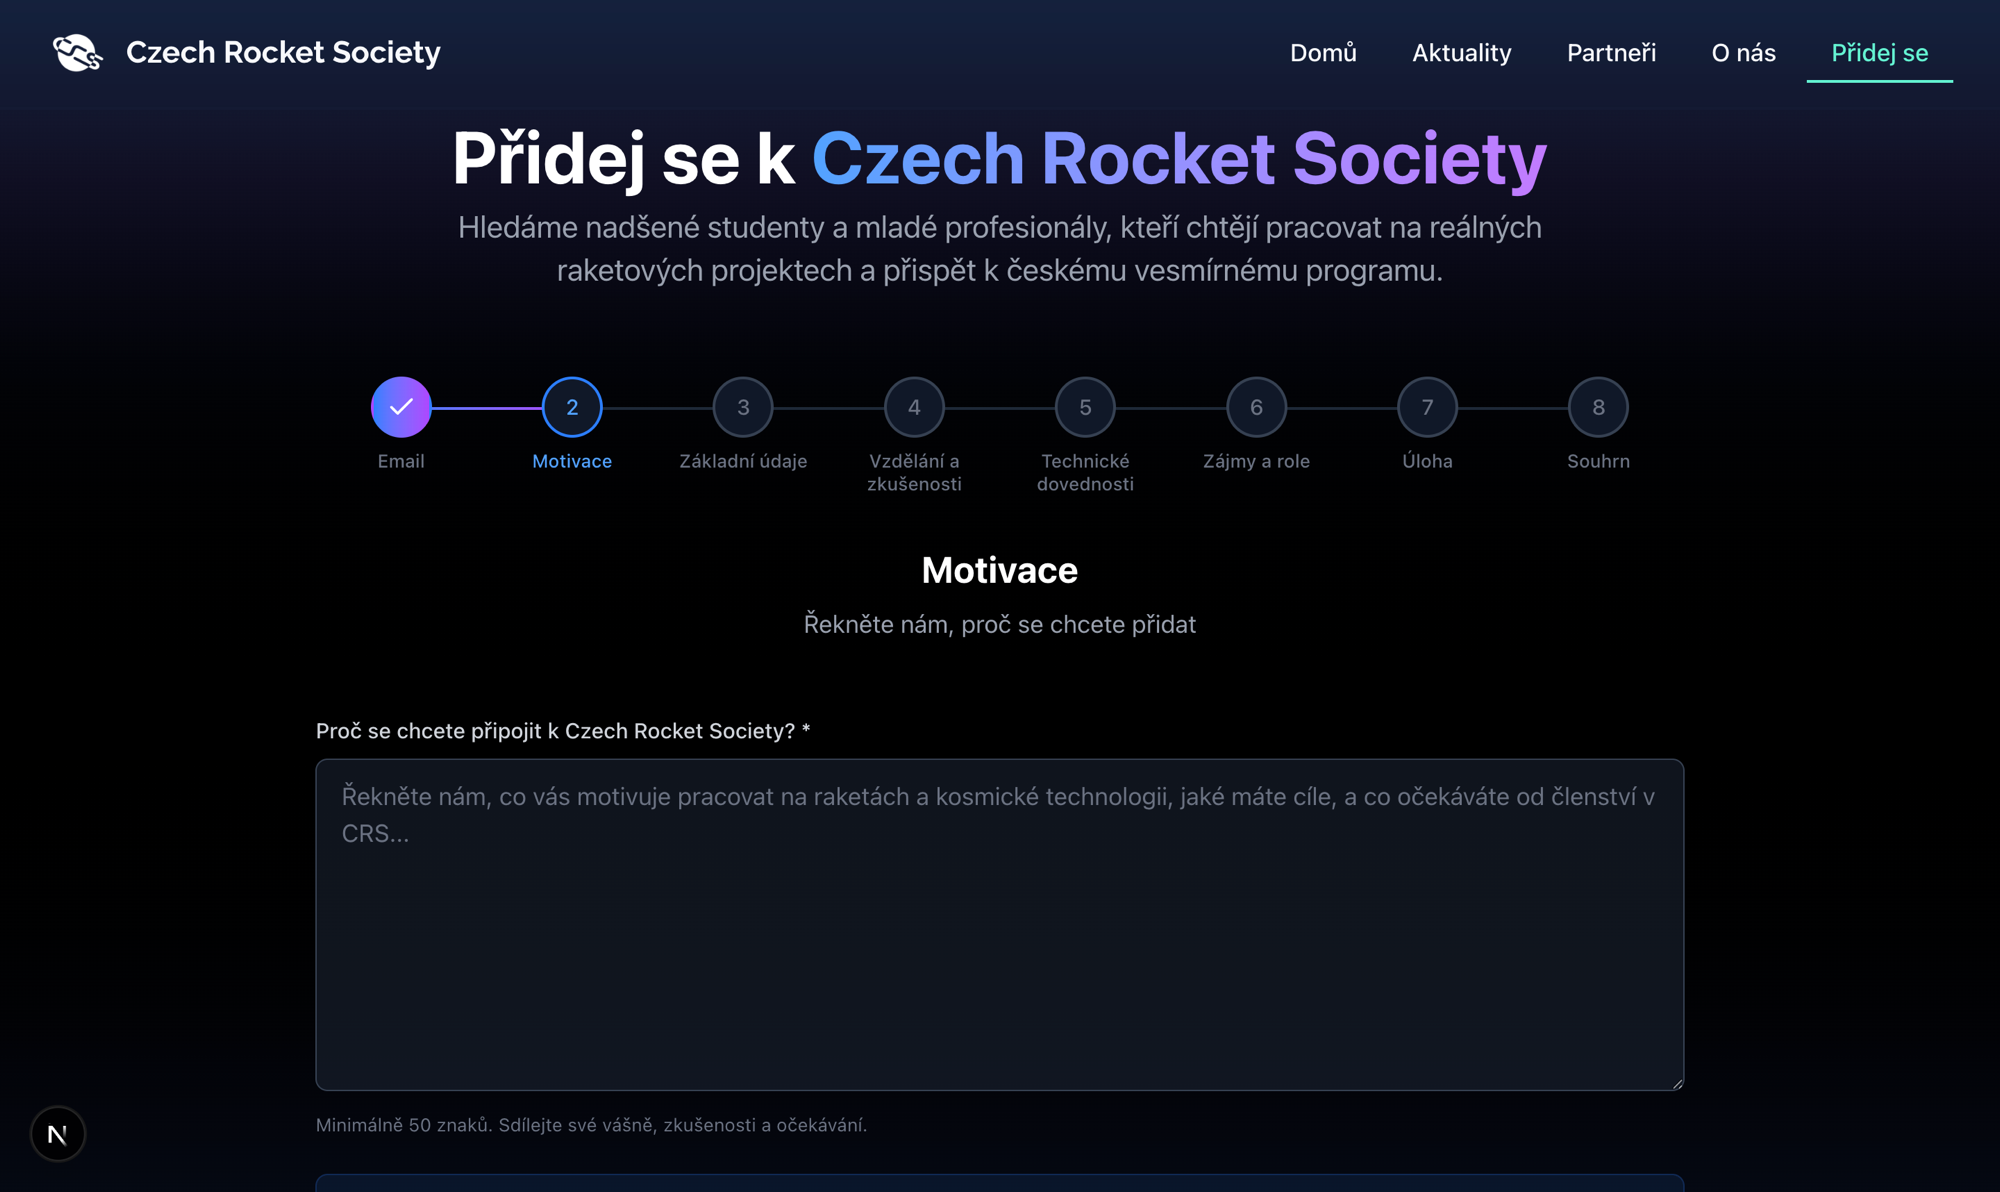
\includegraphics[width=\textwidth]{recruitment-form.png}
\caption{Náborový formulář -- krok motivace s~vizualizací postupu všemi šesti kroky.}
\label{fig:recruitment-form}
\end{figure}

\subsection{Draft systém}

Klíčovým prvkem formuláře je mechanismus průběžného ukládání rozpracované přihlášky. Po zadání e-mailové adresy v~prvním kroku server vytvoří záznam se statusem \texttt{draft} a~odešle uchazeči e-mail s~odkazem pro pokračování. Odkaz obsahuje identifikátor přihlášky a~e-mailovou adresu jako ověřovací parametr.

Změny ve formuláři se automaticky ukládají na server s~dvousekundovým zpožděním (debounce), takže uchazeč nepřijde o~vyplněná data ani při neočekávaném zavření prohlížeče. Při návratu přes odkaz systém detekuje poslední vyplněné pole a~automaticky přesměruje uchazeče na odpovídající krok.

\subsection{Odeslání a~notifikace}

Po kontrole souhrnu v~posledním kroku uchazeč odešle přihlášku, čímž se změní status záznamu z~\texttt{draft} na \texttt{pending}. Systém poté odešle dva e-maily:
\begin{itemize}
    \item \textbf{Uchazeči} -- potvrzení přijetí přihlášky s~informací o~dalším postupu.
    \item \textbf{Administrátorovi} -- notifikace o~nové přihlášce s~přímým odkazem do administrace.
\end{itemize}

\subsection{Administrační workflow}
\label{sec:navrh-nabor-workflow}

Přijaté přihlášky procházejí vícekrokovým workflow, který vede uchazeče od~prvního kontaktu až po~přijetí do~spolku:

\begin{center}
\texttt{pending} $\rightarrow$ \texttt{interview\_scheduled} $\rightarrow$ \texttt{interviewed} $\rightarrow$\\
$\rightarrow$ \texttt{accepted} $\rightarrow$ \texttt{documents\_sent} $\rightarrow$ \texttt{completed}\\
(s~možností přechodu na~\texttt{rejected} v~kterémkoli kroku)
\end{center}

\begin{sloppypar}
V~prvním kroku administrátor zkontroluje doručenou přihlášku (\texttt{pending}). Pokud rozhodne o~jejím postupu, naplánuje uchazeči pohovor zadáním data, na~jehož základě je uchazeči odeslán potvrzovací e-mail; přihláška přejde do~stavu \texttt{interview\-\_scheduled}. Po~uskutečnění pohovoru přepne administrátor přihlášku do~stavu \texttt{inter\-viewed} a~k~záznamu může připojit vlastní poznámky z~rozhovoru. Následné rozhodnutí o~přijetí převede přihlášku do~stavu \texttt{accepted}, načež jsou uchazeči odeslány onboardingové dokumenty (přihláška do~spolku, GDPR souhlas) a~stav se mění na~\texttt{documents\-\_sent}. Po~doručení podepsaných dokumentů uzavře administrátor proces stavem \texttt{completed}, čímž je uchazeč přijat za~člena spolku. V~kterémkoli kroku lze přihlášku zamítnout (\texttt{rejected}) s~uvedením důvodu, který je uchazeči odeslán e-mailem.
\end{sloppypar}

Administrátor vidí seznam přihlášek s~možností filtrování podle statusu a~vyhledávání podle jména nebo e-mailu. V~detailu přihlášky je workflow vizualizován jako pipeline znázorňující aktuální fázi a~předchozí kroky včetně jejich časových razítek. Přidávat lze také interní poznámky viditelné pouze administrátorům. Po~dokončení procesu (\texttt{completed}) je z~dat přihlášky automaticky vytvořen nový člen spolku s~předvyplněnými kontaktními údaji. Toto rozhraní zároveň otevírá do~budoucna možnost navázat na~dokončený nábor automatizovaný onboarding do~dalších platforem, které spolek využívá. 

\subsection{Konfigurovatelné role a~úkoly}

Dostupné role ve spolku a~úkoly pro uchazeče nejsou pevně zakódované, ale uložené jako JSONB struktury v~tabulce \texttt{recruitment\_settings}. Administrátor je může upravovat bez zásahu do kódu -- přidávat nové role s~popisem, definovat úkoly včetně odhadovaného času na vypracování a~přiřazovat je k~jednotlivým rolím. Formulář poté dynamicky zobrazuje relevantní úkol podle zvoleného zájmu uchazeče.

\section{Návrh telemetrického systému}
\label{sec:navrh-telemetrie}

Telemetrický systém zajišťuje přenos dat ze senzorů rakety přes pozemní stanici až do prohlížeče operátora. Návrh klade důraz na nízkou latenci, schopnost zpracovávat vysokofrekvenční datové toky a~současně ukládat veškerá data pro zpětnou analýzu. Celkový tok dat znázorňuje obrázek~\ref{fig:telemetry-flow}.

\begin{figure}[H]
\centering
\begin{tikzpicture}[
    node distance=1.6cm,
    comp/.style={rectangle, draw, rounded corners, minimum height=1.0cm, minimum width=2.5cm, align=center, font=\small, fill=blue!8},
    infra/.style={rectangle, draw, rounded corners, minimum height=1.0cm, minimum width=2.5cm, align=center, font=\small, fill=gray!15},
    ext/.style={rectangle, draw, rounded corners, dashed, minimum height=1.0cm, minimum width=2.5cm, align=center, font=\small},
    arr/.style={-{Stealth[length=3mm]}, thick},
    lbl/.style={font=\footnotesize, fill=white, inner sep=1.5pt}
]
    % Původní vertikální layout
    \node[ext] (rocket) {Raketa\\{\footnotesize (senzory)}};
    \node[ext, below=of rocket] (ground) {Pozemní stanice};
    \node[infra, below=of ground] (mqtt) {Mosquitto\\{\footnotesize (MQTT broker)}};
    \node[comp, below=2.8cm of mqtt] (subscriber) {MQTT subscriber};
    \node[comp, below left=1.6cm and 1.5cm of subscriber] (writer) {InfluxDB writer};
    \node[comp, below right=1.6cm and 1.5cm of subscriber] (wshub) {WebSocket hub};
    \node[infra, below=1.6cm of writer] (influx) {InfluxDB};
    \node[ext, below=1.6cm of wshub] (browser) {Prohlížeč\\{\footnotesize (operátor)}};

    % Dashed box — Go server
    \begin{pgfonlayer}{background}
        \node[draw, dashed, rounded corners, inner sep=0.5cm,
              fit=(subscriber)(writer)(wshub),
              label={[font=\footnotesize\bfseries, anchor=south west, xshift=0.2cm]above right:Go telemetrický server}] {};
    \end{pgfonlayer}

    % Arrows — hlavní tok (kanál A)
    \draw[arr, dashed] (rocket) -- node[lbl, right] {rádio} (ground);
    \draw[arr] (ground) -- node[lbl, right] {MQTT publish} (mqtt);
    \draw[arr] (mqtt) -- node[lbl, right] {subscribe} (subscriber);
    \draw[arr] (subscriber) -- node[lbl, left, pos=0.4] {batch} (writer);
    \draw[arr] (subscriber) -- node[lbl, right, pos=0.4] {broadcast} (wshub);
    \draw[arr] (writer) -- node[lbl, left] {write} (influx);
    \draw[arr] (wshub) -- node[lbl, right] {kanál A} (browser);
    \draw[arr, dashed] (influx) -- node[lbl, below] {REST API (historie)} (browser);

    % Kanál B — přímý MQTT-over-WebSocket z brokeru do prohlížeče
    \draw[arr, densely dotted]
        (mqtt.east) -- ++(6.0cm,0) node[lbl, above] {kanál B (MQTT-over-WS)}
        -- ++(0,-9.2cm) -- (browser.east);

\end{tikzpicture}
\caption{Tok telemetrických dat od~rakety po~prohlížeč operátora. Kanál~A prochází Go~serverem, kanál~B spojuje prohlížeč přímo s~brokerem MQTT.}
\label{fig:telemetry-flow}
\end{figure}

\subsection{MQTT komunikace}

Telemetrická data jsou z~rakety nebo testovacího standu přenášena do systému prostřednictvím protokolu MQTT. Volba MQTT vychází z~vlastností popsaných v~teoretické části -- protokol je navržen pro nespolehlivé sítě s~omezenou šířkou pásma~\cite{mqtt2014oasis}, což odpovídá podmínkám při raketových startech, kde pozemní stanice komunikuje s~raketou přes rádiový kanál a~přeposílá data na server.

Komunikace využívá vzor publish/subscribe~\cite{quincozes2019mqtt}, ve kterém pozemní stanice publikuje zprávy na pojmenované topiky (kanály) a~telemetrický server je odebírá prostřednictvím MQTT brokeru Mosquitto. Oproti přímému HTTP přenosu, který používalo předchozí řešení spolku, tento model přináší několik výhod: producent a~konzument dat se nemusí vzájemně znát, broker zajišťuje doručení i~při dočasném výpadku jedné strany a~jeden datový tok může současně konzumovat více klientů bez duplikace na straně producenta.

\paragraph{Topic hierarchie}

Topiky sledují hierarchickou strukturu umožňující filtrování dat na úrovni brokeru:

\begin{center}
\small\texttt{\{session\_id\}/\{device\_type\}/\{device\_id\}/telemetry/\{data\_type\}}
\end{center}

\noindent Jednotlivé segmenty nesou následující význam:
\begin{sloppypar}
\begin{itemize}
    \item \texttt{session\_id} -- identifikátor konkrétního letu nebo testu (například \texttt{launch-\allowbreak 2026-03-15}),
    \item \texttt{device\_type} -- typ zařízení: \texttt{rocket} (raketa) nebo \texttt{test-stand} (testovací stand),
    \item \texttt{device\_id} -- unikátní identifikátor konkrétního zařízení,
    \item \texttt{data\_type} -- kategorie měřených dat: \texttt{position} (poloha), \texttt{velocity} (rychlost) nebo \texttt{sensors} (senzorická data).
\end{itemize}
\end{sloppypar}

\begin{sloppypar}
Telemetrický server se přihlašuje k~odběru pomocí wildcard vzorů \texttt{+/\allowbreak rocket/\allowbreak +/\allowbreak telemetry/\allowbreak \#} a~\texttt{+/\allowbreak test-stand/\allowbreak +/\allowbreak telemetry/\allowbreak \#}, kde \texttt{+} zastupuje libovolný jeden segment a~\texttt{\#} libovolný počet segmentů~\cite{mqtt2014oasis}. Tím server automaticky zachytává data ze~všech sessions a~zařízení bez nutnosti ruční konfigurace při každém startu.
\end{sloppypar}

\paragraph{Formát zpráv}

Payload každé MQTT zprávy je JSON objekt s~dynamickými poli odpovídajícími měřeným veličinám. Například zpráva typu \texttt{position} obsahuje pole \texttt{alt} (výška), \texttt{lat} a~\texttt{lon} (GPS souřadnice), zpráva typu \texttt{sensors} pak \texttt{temp} (teplota), \texttt{pressure} (tlak), \texttt{battery} (stav baterie) a~\texttt{gyro} (orientace). Volitelné pole \texttt{ts} obsahuje časové razítko z~palubního počítače v~milisekundách od~epochy. Vlastním časovým razítkem datového bodu v~InfluxDB je vždy čas příjmu zprávy serverem; pokud payload obsahuje pole \texttt{ts}, server jej uloží jako pomocné pole \texttt{device\_ts} a~automaticky dopočítá latenci přenosu (\texttt{latency\_ms}) jako rozdíl obou časů.

Dynamická struktura payloadu umožňuje přidávat nové typy senzorů bez úprav serveru -- jakékoli klíče obsažené v~JSON objektu jsou automaticky zapsány jako pole datového bodu do InfluxDB.

\paragraph{Kvalita doručení}

Pro telemetrická data je zvolena úroveň QoS~1 (at least once)~\cite{mqtt2014oasis}. Při nedoručení zprávy klient automaticky provede opakovaný přenos po obnovení spojení, což zajišťuje kompletnost dat i~při nestabilním připojení pozemní stanice~\cite{kegenbekov2022mqtt}. Případné duplicitní doručení nepředstavuje problém -- InfluxDB přepíše datový bod se stejným časovým razítkem. Úroveň QoS~1 musí být nastavena konzistentně na publisheru i~subscriberu, protože efektivní QoS odpovídá minimu z~obou stran~\cite{mqtt2014oasis}.

Vlastní benchmark popsaný v~sekci~\ref{sec:qos-benchmark} ukazuje, že QoS~0 a~QoS~1 dosahují při frekvencích 10--50\,Hz srovnatelné latence (přibližně 46--66\,ms) bez ztrát, zatímco QoS~2 vykazuje dvojnásobnou latenci a~při vyšších frekvencích významné ztráty.

\subsection{Go telemetrický server}

Jádrem telemetrického systému je server napsaný v~Go, který plní tři souběžné úlohy: \textbf{MQTT subscriber} (příjem dat z~MQTT brokeru), \textbf{InfluxDB writer} (perzistence do časové databáze) a~\textbf{WebSocket hub} (distribuce v~reálném čase připojeným klientům). Každá úloha běží jako samostatná goroutina, což umožňuje zpracovávat všechny tři operace paralelně bez vzájemného blokování.

\paragraph{MQTT subscriber}

Subscriber se při spuštění přihlásí k~odběru wildcard topiků na MQTT brokeru a~každou přijatou zprávu parsuje -- z~topiku extrahuje session, typ zařízení, identifikátor a~kategorii dat, z~payloadu dekóduje JSON s~měřenými hodnotami. Výslednou strukturu předá současně oběma dalším komponentám prostřednictvím Go kanálů (channels).

\paragraph{InfluxDB writer}

Writer ukládá přijatá data do časové databáze dávkovým zápisem. Datové body se hromadí v~bufferu a~zapisují se buď po dosažení 500~bodů, nebo po uplynutí 100~ms od posledního zápisu -- podle toho, co nastane dříve. Dávkový zápis výrazně snižuje počet I/O operací oproti zápisu každého bodu jednotlivě a~umožňuje zvládnout vysokou frekvenci příchozích dat bez zahlcení databáze.

\paragraph{WebSocket hub}

Hub spravuje připojení klientů (prohlížečů) a~distribuuje jim telemetrická data v~reálném čase. Každý klient se při připojení přihlásí k~odběru konkrétní session a~hub mu odesílá pouze relevantní data. Pro snížení síťové režie hub sdružuje zprávy do mikrodávek a~implementuje mechanismus zpětného tlaku (backpressure) pro případ, že klient nestíhá zprávy přijímat. Implementační detaily mikrodávkování a~backpressure jsou popsány v~kapitole~\ref{chap:implementace}.

\subsection{Dual-channel architektura}

Prohlížeč má k~dispozici dva nezávislé kanály pro příjem telemetrických dat:

\begin{enumerate}
    \item \textbf{Kanál~A -- Go WebSocket.} Data procházejí Go serverem, který je sdružuje do mikrodávek, filtruje podle session a~řídí backpressure. Tento kanál poskytuje optimalizovaný a~stabilní tok dat.
    \item \textbf{Kanál~B -- přímý MQTT-over-WebSocket.} Prohlížeč se připojí přímo k~Mosquitto brokeru na portu 9001 a~odebírá surová MQTT data bez zprostředkování Go serverem. Tento kanál funguje nezávisle na telemetrickém serveru, takže data proudí i~při jeho výpadku.
\end{enumerate}

Operátor si volí režim příjmu dat prostřednictvím přepínače ve stavové liště: pouze kanál~A, pouze kanál~B (výchozí), nebo oba současně pro porovnání výkonnosti. Výchozím kanálem je B, protože nevyžaduje běžící Go server a~umožňuje okamžité sledování dat ihned po spuštění MQTT brokeru. Oba kanály implementují nezávislou reconnect logiku s~exponenciálním zpožděním při výpadku spojení.

\subsection{Telemetrický dashboard}

Dashboard v~prohlížeči pracuje ve dvou režimech:

\textbf{Live režim} zobrazuje data z~probíhajícího letu v~reálném čase. Rozhraní obsahuje časové grafy klíčových veličin (výška, rychlost, zrychlení), GPS mapu s~trajektorií letu, panely s~aktuálními hodnotami senzorů (teplota, tlak, stav baterie) a~indikátor aktuální fáze letu (odpočet, vzlet, stoupání, let setrvačností, apogeum, sestup, přistání).

\textbf{Historie} zobrazuje statické grafy zaznamenaného letu (výška, rychlost, teplota, tlak) načtené z~InfluxDB prostřednictvím REST API s~podporou downsamplingu -- uživatel volí rozlišení dat (od surových až po 30sekundové agregace) a~server automaticky agreguje data, aby se snížil objem přenášených bodů. Data lze exportovat do formátu CSV nebo JSON.

\subsection{Simulátor}

Pro vývoj a~testování telemetrického systému bez nutnosti fyzického raketového startu slouží simulátor -- samostatný Go program, který generuje realistická telemetrická data a~publikuje je na MQTT broker ve stejném formátu jako skutečná pozemní stanice.

Simulátor modeluje průběh letu včetně jednotlivých fází (odpočet, vzlet, stoupání, let setrvačností, apogeum, sestup, přistání) a~pro každou fázi generuje odpovídající hodnoty -- stoupající výšku a~rychlost při vzletu, pokles teploty s~rostoucí výškou, úbytek baterie v~čase a~šum gyroskopu. Konfigurovatelné parametry zahrnují frekvenci vysílání (Hz), identifikátor session a~délku simulovaného letu.

\section{Bezpečnost}
\label{sec:navrh-bezpecnost}

Bezpečnostní opatření platformy pokrývají tři oblasti: autentizaci uživatelů při přístupu do administrace, ochranu API endpointů před neoprávněným zápisem a~bezpečné ukládání citlivých údajů.

\subsection{Autentizační tok}

Přihlášení do administrace prochází dvěma systémy -- NextAuth na frontendu a~vlastní JWT autentizací na backendu. Celý tok probíhá v~následujících krocích:

\begin{enumerate}
    \item Uživatel zadá e-mail a~heslo na přihlašovací stránce (\texttt{/admin/login}).
    \item NextAuth prostřednictvím \texttt{Credentials\-Provider} odešle požadavek \texttt{POST\allowbreak{} /api/\allowbreak auth/\allowbreak login} na~backend API.
    \item Backend vyhledá uživatele v~databázi podle e-mailu a~ověří heslo porovnáním s~uloženým hashem pomocí \texttt{bcrypt.compare}.
    \item Při úspěšném ověření backend vygeneruje JWT token s~payloadem obsahujícím identifikátor uživatele, e-mail a~roli. Token má platnost 7~dní.
    \item NextAuth přijme token a~uloží jej prostřednictvím callbacků -- \texttt{jwt()} callback přenese backend token do session a~\texttt{session()} callback jej zpřístupní klientské aplikaci.
    \item Session je uložena v~httpOnly cookie, kterou prohlížeč automaticky odesílá při každém požadavku.
\end{enumerate}

Při následných požadavcích na chráněné API endpointy frontend přiloží backend JWT token v~hlavičce \texttt{Authorization: Bearer <token>}. Middleware na straně API token ověří a~extrahuje identitu uživatele.

Next.js middleware chrání všechny cesty pod \texttt{/admin/*} -- nepřihlášeného uživatele přesměruje na přihlašovací stránku, přihlášeného uživatele přesměruje z~přihlašovací stránky na dashboard.

Pro komunikaci mezi frontendem a~backendem v~Docker prostředí se používají dvě adresy: server-side požadavky (při přihlašování) využívají interní Docker adresu (\texttt{INTERNAL\_API\_URL}), zatímco klientské požadavky z~prohlížeče používají veřejnou adresu (\texttt{NEXT\_PUBLIC\_API\_URL}).

\subsection{Ochrana API}

Každý požadavek na API prochází řetězcem middleware funkcí v~pořadí: logger (záznam požadavků) $\rightarrow$ CORS -- Cross-Origin Resource Sharing (kontrola původu) $\rightarrow$ případný \texttt{authMiddleware} (ověření tokenu) $\rightarrow$ handler (zpracování požadavku).

CORS middleware povoluje požadavky pouze z~nakonfigurovaných domén (\texttt{CORS\-\_ORIGIN}) a~vyžaduje příznak \texttt{credentials:\allowbreak{} true} pro odesílání autentizačních hlaviček. Tím se na~úrovni prohlížeče zabraňuje tomu, aby skripty běžící na~cizích doménách komunikovaly s~API. CORS slouží primárně jako ochrana koncového uživatele v~prohlížeči; samotná autorizace API je zajišťována JWT middlewarem.

Validace vstupních dat prostřednictvím Zod schémat na všech POST a~PUT endpointech zajišťuje, že API nepřijme neočekávaná nebo neplatná data. Validace probíhá ještě před zpracováním požadavku, čímž se snižuje riziko chyb na úrovni databáze.

\subsection{Ukládání hesel}

Hesla uživatelů jsou hashována algoritmem bcrypt s~cost faktorem 10 (tj. $2^{10}$ iterací klíčového rozvrhu) a~automaticky generovanou solí. V~databázi se ukládá výhradně výsledný hash -- původní heslo nelze z~hashe rekonstruovat. Při ověřování se zadané heslo hashuje se stejnou solí a~výsledek se porovnává s~uloženým hashem.

\chapter{Implementace}
\label{chap:implementace}

Tato kapitola popisuje implementaci jednotlivých částí platformy -- od vývojového prostředí přes backend a~frontend až po telemetrický systém a~kontejnerizaci. Důraz je kladen na klíčová technická rozhodnutí a~vzory, které se opakují napříč celou aplikací.

\section{Vývojové prostředí a~nástroje}

Vývoj probíhá v~editoru \textbf{VS Code} za~pomoci nástroje \textbf{Claude Code} pro generování kódu, refaktoring a~hromadné úpravy napříč projektem. Verzování zajišťuje \textbf{Git} s~repozitářem na~GitHubu.

Jako správce balíčků slouží \textbf{pnpm}, který byl zvolen pro nativní podporu workspaces potřebnou pro monorepo strukturu a~sdílené úložiště balíčků, díky kterému se závislosti na~disku neduplikují. Pro běh TypeScript kódu bez předchozí kompilace se používá \textbf{tsx} -- runtime, který transpiluje TypeScript za~běhu a~podporuje moduly ECMAScript (ESM). Toto řešení bylo zvoleno proto, že kompilátor \texttt{tsc} při výstupu do~ESM nepřidává přípony \texttt{.js} k~importům, což v~Node.js vede k~runtime chybě (\texttt{ERR\_\allowbreak MODULE\_\allowbreak NOT\_\allowbreak FOUND}).

Infrastrukturní služby (PostgreSQL, InfluxDB, Mosquitto, MailHog) běží v~\textbf{Docker} kontejnerech, což zajišťuje konzistentní prostředí bez nutnosti lokální instalace jednotlivých služeb.

\section{Struktura monorepa}

Repozitář je organizován jako monorepo s~následující adresářovou strukturou:

\begin{verbatim}
+-- apps/
|   +-- api/          # Hono REST API (TypeScript, Node.js)
|   +-- web/          # Next.js frontend (React, TypeScript)
|   +-- telemetry/    # Go telemetricky server
+-- docker/           # Docker Compose konfigurace
+-- pnpm-workspace.yaml
\end{verbatim}

Soubor \texttt{pnpm-workspace.yaml} definuje \texttt{apps/*} jako workspace balíčky. Díky tomu lze spouštět příkazy pro všechny aplikace najednou (\texttt{pnpm dev} spustí paralelně frontend i~backend) nebo cíleně pro jednu aplikaci (\texttt{pnpm --filter api build}).

\section{Backend -- Hono API}

\subsection{Middleware a routing}

\begin{sloppypar}
Vstupní bod backendu je soubor \texttt{server.ts}, kde se inicializuje instance Hono, konfiguruje řetězec middleware popsaný v~sekci~\ref{sec:navrh-bezpecnost} a~připojují se route handlery. Každá skupina endpointů (články, události, projekty apod.) je implementována jako samostatná Hono instance v~adresáři \texttt{src/\allowbreak routes/} a~připojena metodou \texttt{app.route()} na~vlastní prefix začínající \texttt{/api} (například \texttt{app.route(\allowbreak '/api/\allowbreak articles',\allowbreak{} articles\-Router)}). API dokumentace je přístupná přes Swagger~UI na~cestě \texttt{/docs} s~OpenAPI~3.0 specifikací.
\end{sloppypar}

\subsection{Databázová vrstva -- Drizzle ORM}

Připojení k~databázi je konfigurováno v~souboru \texttt{src/db/index.ts} s~connection poolem. Drizzle ORM generuje typově bezpečné SQL dotazy přímo z~TypeScriptového schématu.

Typický CRUD vzor na příkladu článků:

\begin{sloppypar}
\begin{itemize}
    \item \textbf{Čtení:} \texttt{db.select().from(articles).\allowbreak where(\allowbreak eq(\allowbreak articles.status,\allowbreak{} 'published'))}
    \item \textbf{Vytvoření:} \texttt{db.insert(articles).\allowbreak values(data).\allowbreak returning()} -- metoda \texttt{returning()} vrací vložený záznam včetně vygenerovaného UUID.
    \item \textbf{Aktualizace:} \texttt{db.update(articles).\allowbreak set(data).\allowbreak where(\allowbreak eq(\allowbreak articles.id,\allowbreak{} id)).\allowbreak returning()}
    \item \textbf{Smazání:} \texttt{db.delete(articles).\allowbreak where(\allowbreak eq(\allowbreak articles.id,\allowbreak{} id))}
\end{itemize}
\end{sloppypar}

Databázové schéma se synchronizuje příkazem \texttt{pnpm db:push}, který porovná TypeScript definici s~aktuálním stavem databáze a~aplikuje změny. Pro naplnění vývojové databáze testovacími daty slouží příkaz \texttt{pnpm db:seed}.

\subsection{Autentizace a validace}

Autentizační tok a~bezpečnostní mechanismy jsou popsány v~sekci~\ref{sec:navrh-bezpecnost}. Z~hlediska implementace je klíčové rozložení kódu do modulů: \texttt{src/lib/jwt.ts} zapouzdřuje práci s~JWT tokeny (podepisování klíčem z~\texttt{JWT\_SECRET}, ověření podpisu a~expirace), \texttt{src/middleware/auth.ts} obsahuje middleware funkce a~\texttt{src/routes/auth.ts} implementuje přihlašovací a~registrační endpoint.

Validační Zod schémata jsou oddělena do adresáře \texttt{src/schemas/} a~integrována s~Hono prostřednictvím \texttt{@hono/zod-validator}, který je aplikuje jako middleware před samotným route handlerem. Díky tomu handler vždy obdrží typově ověřená data.

\subsection{Nahrávání souborů}

\begin{sloppypar}
Nahrávání souborů popsané v~sekci~\ref{sec:navrh-upload} je implementováno ve~dvou modulech: \texttt{upload.ts} pro obecné nahrávání a~\texttt{media.ts} pro správu knihovny médií. Soubory jsou zpracovány vestavěnou metodou \texttt{c.req.\allowbreak parseBody()} frameworku Hono. V~knihovně médií jsou názvy souborů generovány pomocí UUID, čímž se předchází kolizím při současném nahrávání více souborů; v~obecném upload endpointu se používá časové razítko jako jednodušší varianta.
\end{sloppypar}

\subsection{E-mailový systém}

E-maily jsou odesílány knihovnou Nodemailer přes SMTP (Simple Mail Transfer Protocol) server. Ve vývojovém prostředí slouží jako SMTP server MailHog, který zachytává všechny odeslané e-maily a~zobrazuje je ve webovém rozhraní bez skutečného doručení.

E-mailové šablony jsou implementovány jako funkce vracející HTML řetězec s~tabulkovým layoutem pro kompatibilitu s~e-mailovými klienty. Platforma odesílá tři typy e-mailů: odkaz pro pokračování v~rozpracované přihlášce, potvrzení odeslání přihlášky a~notifikaci administrátora o~nové přihlášce.

\section{Frontend -- Next.js}

\subsection{Veřejné stránky}

Veřejné stránky využívají App Router v~režimu serverových komponent -- data se načítají přímo na serveru při každém požadavku (\texttt{dynamic = 'force-dynamic'}). API klient v~souboru \texttt{lib/api.ts} detekuje prostředí (server vs.~prohlížeč) a~volí odpovídající URL -- na serveru interní Docker adresu, v~prohlížeči veřejnou adresu.

Stránky s~dynamickým obsahem (články, události, projekty) používají v~URL slug popsaný v~sekci~\ref{sec:navrh-verejne-stranky}.

\subsection{Administrační rozhraní}

Administrace je implementována jako route group \texttt{(dashboard)} se sdíleným layoutem. Layout obsahuje horní lištu s~informacemi o~přihlášeném uživateli a~tlačítkem pro odhlášení a~postranní navigační panel se sekcemi vyjmenovanými v~sekci~\ref{sec:navrh-verejne-stranky}. Aktivní položka je zvýrazněna na základě aktuální URL cesty.

CRUD formuláře jsou postaveny na knihovně React Hook Form s~Zod validací. Formulář pro články navíc obsahuje automatické generování slugu z~názvu a~rich-text editor pro formátování obsahu.

\paragraph{Rich-text editor}
\label{sec:impl-richtext}

Pro formátování obsahu článků, událostí a~projektů slouží rich-text editor postavený na knihovně \textbf{Tiptap} -- moderním editoru založeném na ProseMirror. Editor je integrován jako React komponenta \texttt{RichTextEditor} s~hookem \texttt{useEditor}, který spravuje stav editoru a~při každé změně vrací obsah jako standardní HTML string.

Toolbar obsahuje všechny běžné formátovací nástroje potřebné pro tvorbu strukturovaného obsahu. Tlačítka jsou implementována jako SVG (Scalable Vector Graphics) ikony s~vizuálním zvýrazněním aktivního stavu -- editor při každé transakci aktualizuje stav tlačítek včetně situace, kdy uživatel aktivuje formátování na prázdném řádku (tzv. stored marks).

Obsah je uložen v~databázi jako HTML řetězec a~na~veřejných stránkách vykreslen s~odpovídajícím stylováním. Volba knihovny Tiptap a~důvody migrace z~původního řešení jsou popsány v~sekci~\ref{sec:test-richtext}. Ukázka editoru v~administračním rozhraní je zachycena na~obrázku~\ref{fig:richtext-editor}.

\begin{figure}[H]
\centering
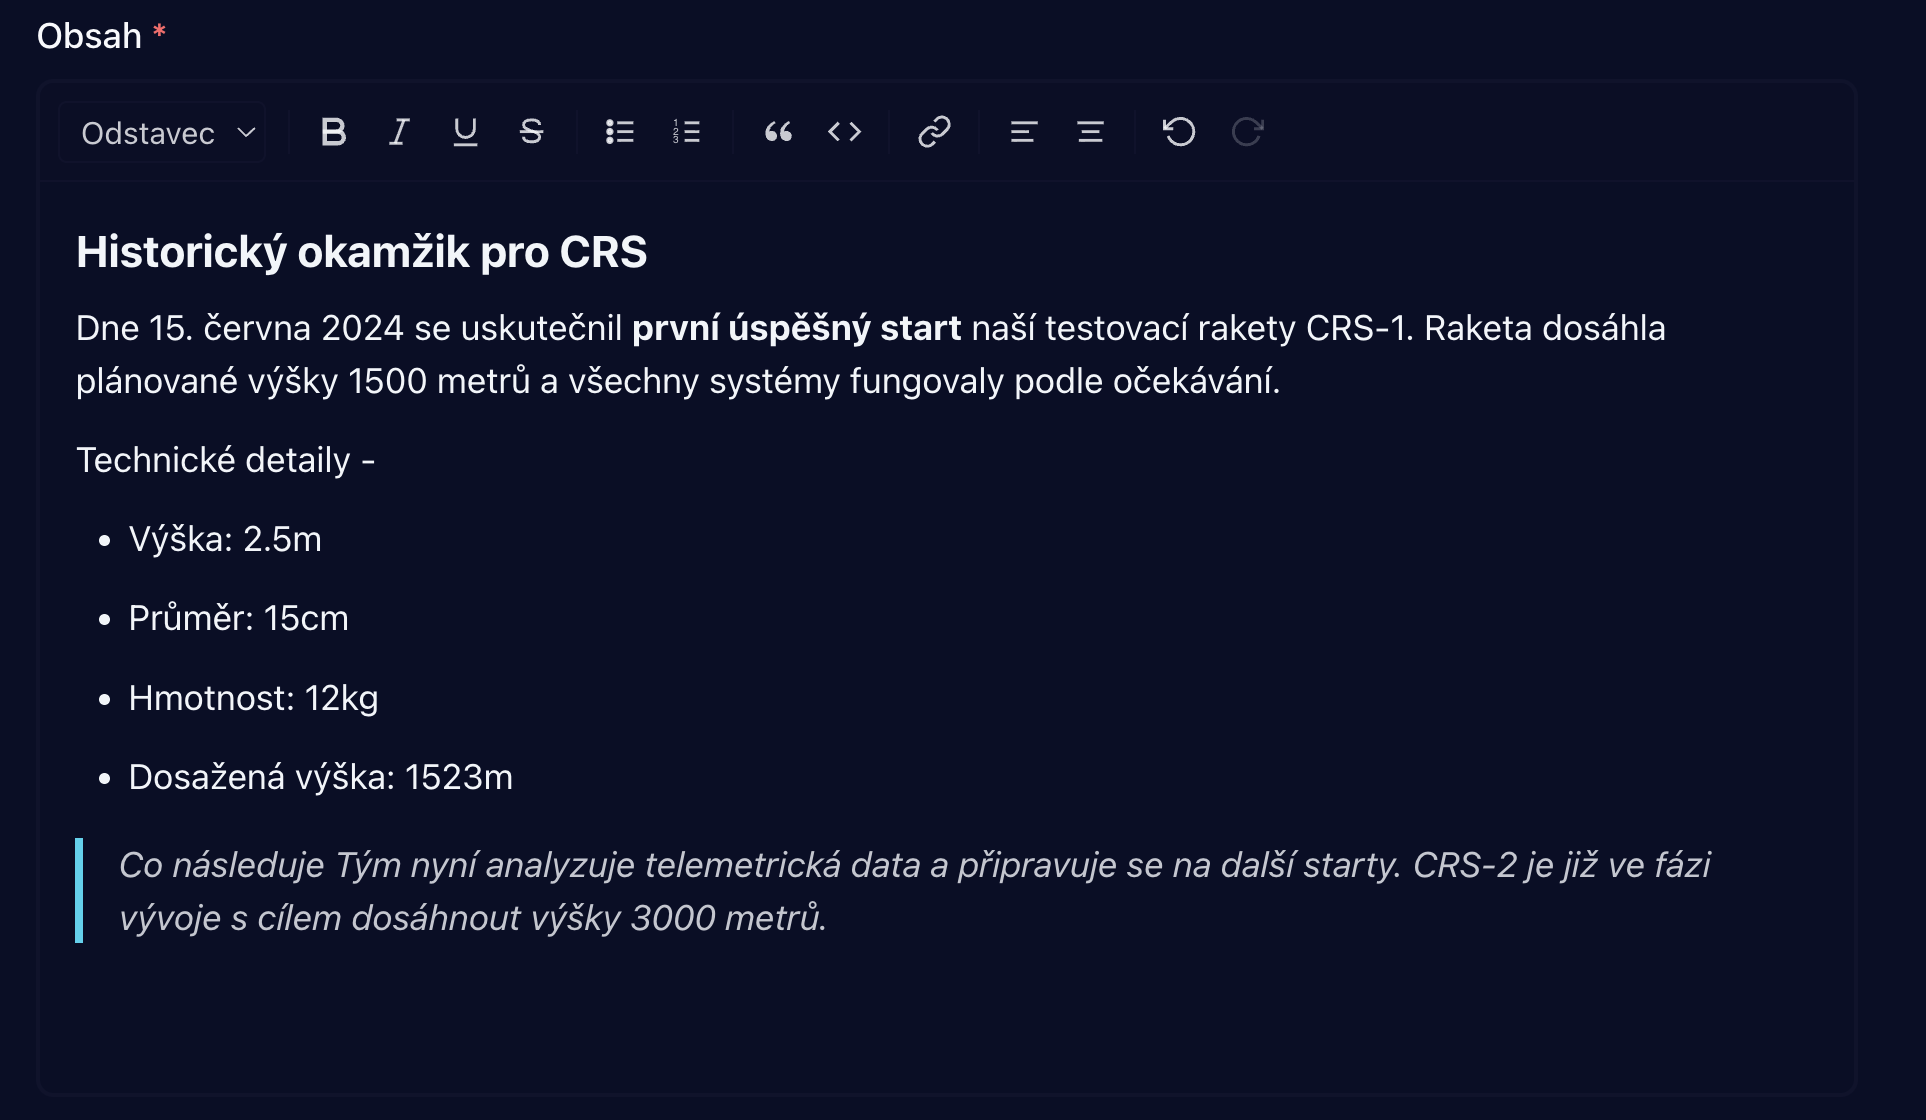
\includegraphics[width=\textwidth]{richtext-editor.png}
\caption{Rich-text editor Tiptap v~administraci s~toolbarem a~ukázkou formátovaného obsahu.}
\label{fig:richtext-editor}
\end{figure}

\paragraph{Knihovna médií}

Komponenta \texttt{ImageUploader} slouží jako galerie nahraných obrázků s~možností nahrávání nových souborů. Při vkládání obrázku do obsahu (např.~náhled článku) se otevře modální okno \texttt{ImagePickerModal}, ve kterém uživatel vybere existující obrázek z~knihovny nebo nahraje nový. Vybraný obrázek je zvýrazněn tyrkysovým okrajem.

\subsection{Autentizace na frontendu}

Autentizační tok mezi frontendem a~backendem je popsán v~sekci~\ref{sec:navrh-bezpecnost}. Implementačně je konfigurace NextAuth v5 umístěna v~souboru \texttt{lib/auth.ts}, kde jsou definovány callbacky \texttt{jwt()} a~\texttt{session()} pro přenos backend tokenu do klientské session. Ochrana administračních rout je zajištěna middleware v~souboru \texttt{middleware.ts}, který pokrývá vzor \texttt{/admin/:path*}.

Specifickým implementačním detailem je nastavení \texttt{trustHost: true}, které je nezbytné pro správnou funkci NextAuth za~reverse proxy v~Docker prostředí -- bez něj NextAuth odmítá požadavky kvůli neshodě mezi hlavičkou \texttt{Host} a~odvozeným base URL.

\subsection{Náborový formulář}

Náborový proces navržený v~sekci~\ref{sec:navrh-nabor} je implementován komponentou \texttt{Recruitment\-Form}. Formulář je řízen stavem \texttt{current\-Step} (0--5) s~jediným \texttt{useForm} hookem spravujícím data všech kroků, přičemž přechody mezi kroky jsou animovány knihovnou Framer Motion.

\begin{sloppypar}
Klíčovým implementačním detailem je automatické ukládání rozpracované přihlášky realizované debouncerem -- \texttt{useEffect} sleduje změny formulářových dat a~po~2~sekundách nečinnosti odešle aktuální stav na~server. Identifikátor draftu a~e-mail jsou uloženy v~URL parametrech (\texttt{?draft=ID\&\allowbreak email=EMAIL}), takže zůstávají zachovány i~po~zavření prohlížeče. Funkce \texttt{get\-Resume\-Step()} analyzuje vyplněná pole v~obráceném pořadí a~vrátí číslo kroku, od~kterého má uchazeč pokračovat.
\end{sloppypar}

Přístup k~rozpracované přihlášce je chráněn kombinací UUID draftu a~e-mailové adresy -- API při načtení ověřuje shodu obou identifikátorů, takže k~datům přihlášky se dostane pouze uchazeč, který obdržel odkaz e-mailem.

Dostupné role a~úkoly formulář načítá při inicializaci z~veřejného API endpointu \texttt{GET\allowbreak{} /api/\allowbreak recruitment/\allowbreak settings/\allowbreak public}, který vrací aktuální konfiguraci z~tabulky \texttt{recruitment\-\_settings} bez nutnosti autentizace. Úkoly se filtrují podle vybrané role uchazeče -- zobrazí se pouze ty, které jsou k~dané roli přiřazeny, případně úkoly bez přiřazení určené všem uchazečům.

\subsection{Design systém a stylování}

Vizuální stránka aplikace je postavena na~frameworku Tailwind CSS~v4 s~vlastní barevnou paletou definovanou jako proměnné CSS. Aktuální paleta používá kosmický motiv (tmavé pozadí \texttt{deep-space}, akcenty \texttt{aurora-cyan} a~\texttt{aurora-blue}), který byl zvolen nezávisle na~oficiální vizuální identitě spolku. V~konfiguračním souboru jsou paralelně definovány i~oficiální barvy CRS (například \texttt{crs-base}, \texttt{crs-ignition}), připravené pro budoucí sjednocení vizuálního stylu se značkou spolku, která se v~době vývoje stále formovala.

Typografie využívá tři fonty načítané přes \texttt{next/font/google}: \textbf{Raleway} pro nadpisy, \textbf{Roboto Slab} jako základní písmo a~\textbf{Comfortaa} pro akcentové prvky. Responzivní design je řešen prostřednictvím Tailwind bodů zlomu -- rozložení se přizpůsobuje šířce obrazovky od~mobilních zařízení po~širokoúhlé monitory. Animace přechodů a~interakcí zajišťuje knihovna Framer Motion.

\section{Telemetrický systém}

\subsection{Go server}

Telemetrický server je strukturován podle konvence Go projektů s~adresáři \texttt{cmd/} pro vstupní body a~\texttt{internal/} pro interní balíčky:

\begin{verbatim}
apps/telemetry/
+-- cmd/
|   +-- server/main.go       # Vstupni bod serveru
|   +-- simulator/main.go    # Vstupni bod simulatoru
+-- internal/
    +-- config/    # Konfigurace z promennych prostredi
    +-- mqtt/      # MQTT subscriber a parsovani topiku
    +-- influx/    # InfluxDB batch writer a dotazy
    +-- ws/        # WebSocket hub a distribuce dat
    +-- api/       # HTTP router (Chi) a REST endpointy
\end{verbatim}

Při spuštění \texttt{main.go} inicializuje všechny komponenty, propojí MQTT subscriber s~InfluxDB writerem a~WebSocket hubem prostřednictvím handler funkcí (každá přijatá zpráva je předána oběma konzumentům přímým voláním) a~spustí HTTP server. WebSocket hub uvnitř pracuje s~Go kanály pro asynchronní distribuci klientům. Při ukončení (signál SIGINT/SIGTERM) proběhne graceful shutdown -- prostřednictvím \texttt{defer} se uzavřou MQTT a~InfluxDB klienti, čímž se dokončí rozpracované dávkové zápisy.

\subsection{MQTT komunikace}

MQTT komunikace navržená v~sekci~\ref{sec:navrh-telemetrie} je implementována v~balíčku \texttt{internal/mqtt}. Registrace handlerů probíhá přes metodu \texttt{OnMessage()}, která umožňuje připojit libovolný počet konzumentů -- v~produkční konfiguraci jsou registrovány dva: InfluxDB writer a~WebSocket hub.

\subsection{WebSocket hub}

WebSocket hub sdružuje zprávy do mikrodávek s~intervalem 16\,ms, který odpovídá obnovovací frekvenci většiny monitorů (60\,Hz) -- prohlížeč překresluje rozhraní prostřednictvím \texttt{request\-Animation\-Frame} přibližně každých 16{,}67\,ms~\cite{mdn2024raf}, takže častější odesílání dat by nepřineslo vizuální zlepšení, zatímco delší interval by způsobil viditelné skoky v~grafech.

Pokud klient nestíhá zprávy přijímat, hub aktivuje mechanismus zpětného tlaku (backpressure) a~starší nedoručené zprávy zahazuje, aby fronta nerostla do nekonečna. Toto zahazování se týká výhradně WebSocket distribuce -- zápis do InfluxDB probíhá nezávislou cestou přímo z~MQTT subscriberu, takže žádná data se v~databázi neztrácejí. Pro uživatele to znamená dočasné snížení rozlišení grafů; po stabilizaci spojení se plné rozlišení automaticky obnoví.

Spojení je udržováno prostřednictvím ping/pong zpráv v~intervalu 30~sekund. Při výpadku spojení se klient automaticky pokusí o~opětovné připojení.

\subsection{Real-time vizualizace v~prohlížeči}

\begin{sloppypar}
Frontendová část telemetrie je organizována kolem React kontextu \texttt{TelemetryProvider}, který spravuje připojení k~datovým kanálům a~zpřístupňuje přijatá data komponentám prostřednictvím custom hooků (\texttt{useGoWebSocket} pro kanál~A, \texttt{useDirectMqtt} pro kanál~B).
\end{sloppypar}

Přijatá data jsou akumulována v~paměti po celou dobu letu -- historické pole pro každou měřenou veličinu (pozice, rychlost, senzory) se neořezávají, takže graf zobrazuje kompletní průběh od začátku příjmu. Pokud data přestanou přicházet déle než jednu sekundu, provider nastaví příznak \texttt{isStale} a~stavová lišta zobrazí varovný indikátor. Grafy v~tomto režimu prodlouží poslední známou hodnotu rovnou čárou do aktuálního času.

Vizualizační komponenty zahrnují časové grafy výšky a~rychlosti (knihovna Recharts) s~osou X synchronizovanou se systémovým časem, obloukové ukazatele aktuálních hodnot senzorů (výška, rychlost, teplota, baterie), GPS mapu s~trajektorií letu (Leaflet s~tmavými mapovými dlaždicemi) včetně vzdálenosti od~místa vzletu, panel maximálních hodnot a~indikátor fáze letu. Stavová lišta umožňuje přepínání kanálů, vymazání dat před novým startem a~doplnění historických dat z~InfluxDB -- operátor se tak může připojit k~probíhajícímu letu a~doplnit si průběh, který zameškal. Ukázka kompletního live dashboardu při běžícím simulátoru je zachycena na~obrázku~\ref{fig:telemetry-live}.

\begin{figure}[H]
\centering
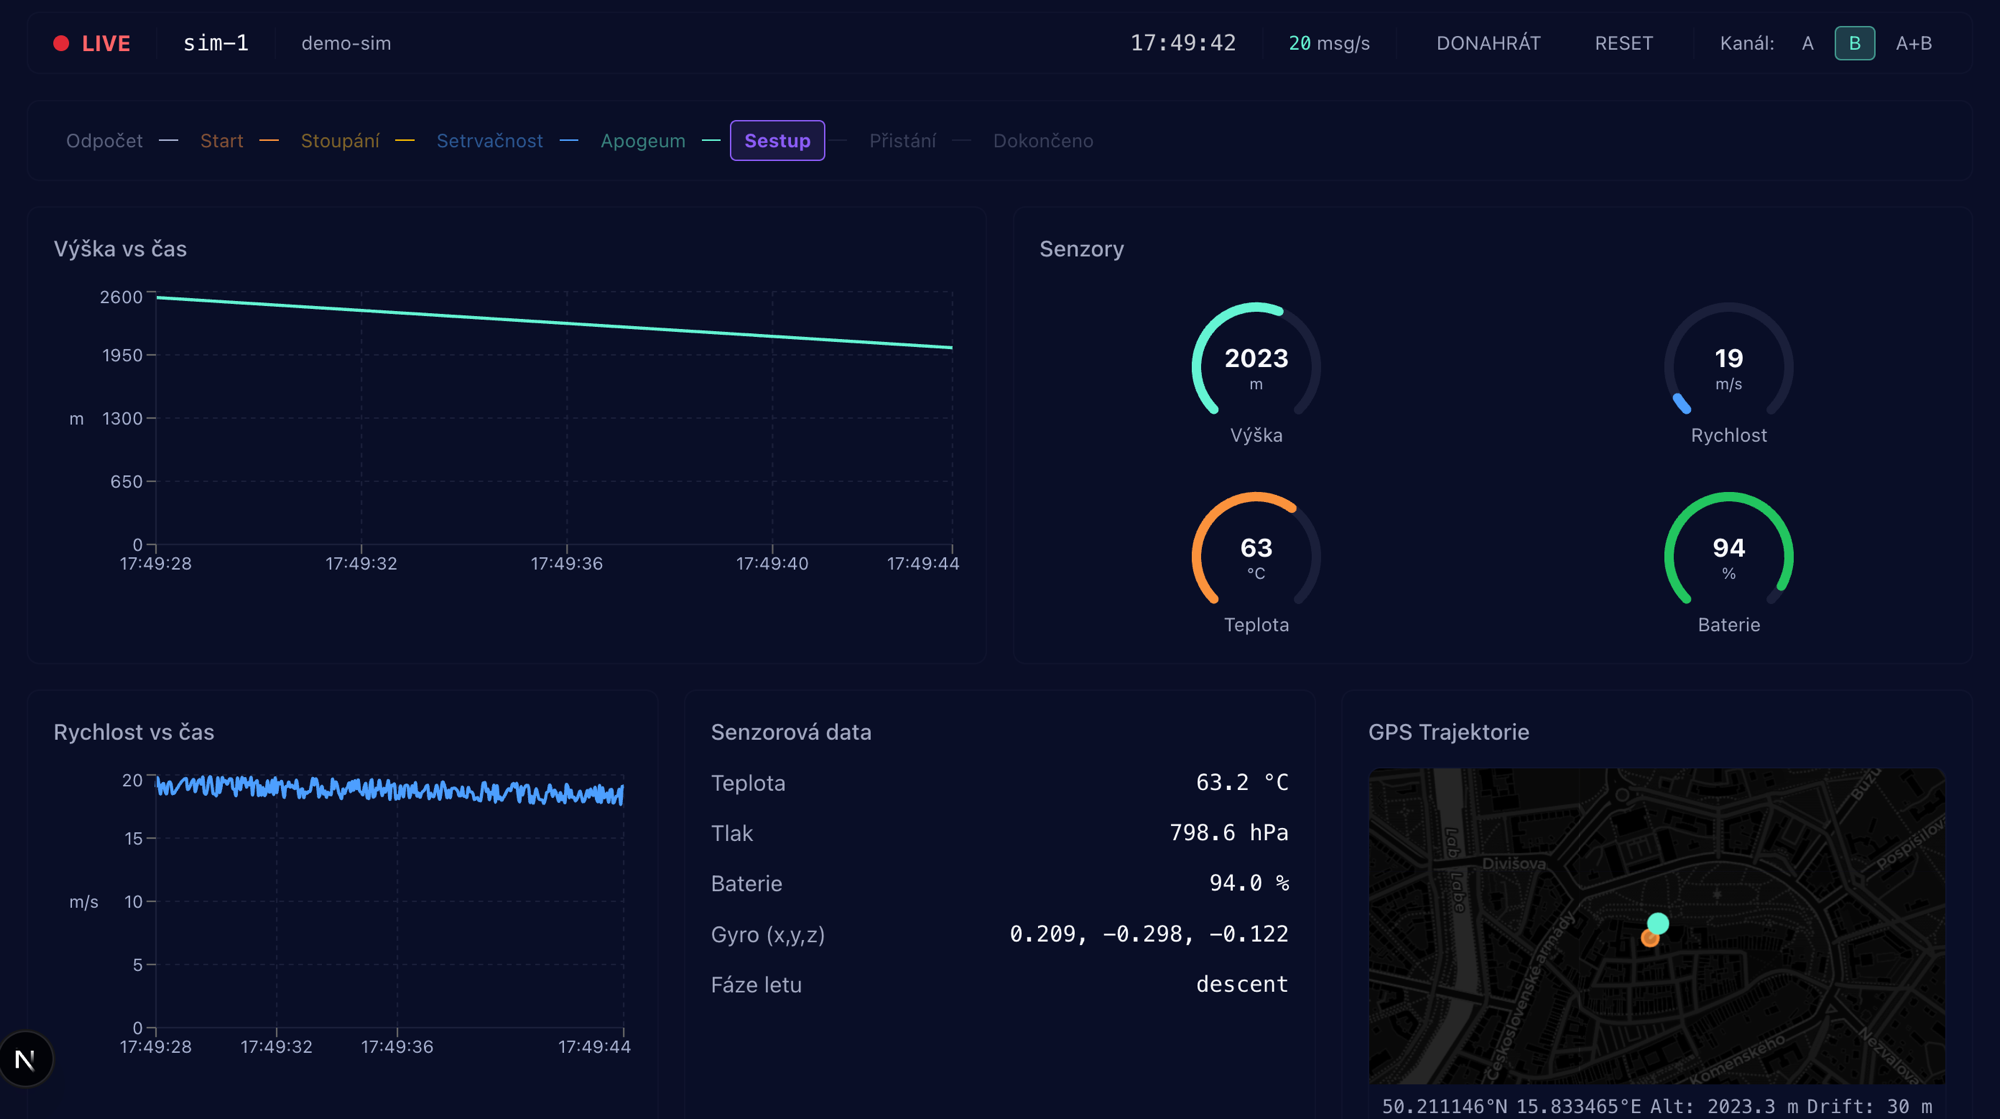
\includegraphics[width=\textwidth]{telemetry-live.png}
\caption{Telemetrický dashboard v~live režimu -- časové grafy výšky a~rychlosti, obloukové ukazatele senzorů, GPS trajektorie a~stavová lišta s~přepínačem kanálů.}
\label{fig:telemetry-live}
\end{figure}

\subsection{Prohlížení historických dat}

Stránka historie zobrazuje statické grafy zaznamenaného letu (výška, rychlost, teplota, tlak) načtené z~InfluxDB prostřednictvím REST API telemetrického serveru. Uživatel volí rozlišení dat (od~surových až~po~30sekundové agregace) -- server použije agregační funkci \texttt{aggregateWindow} pro snížení objemu přenášených bodů. Data lze exportovat do~formátu CSV nebo JSON pro další zpracování a~dlouhodobé ukládání.

\subsection{Simulátor}

Simulátor (\texttt{cmd/simulator/main.go}) generuje realistická telemetrická data modelováním průběhu letu v~sedmi fázích: odpočet, vzlet, stoupání, let setrvačností, apogeum, sestup a~přistání. Pro každou fázi jsou definovány fyzikální vztahy ovlivňující výšku, rychlost, teplotu, tlak a~stav baterie. Gyro data obsahují simulovaný šum pro realističnost. Simulátor podporuje také simulaci výpadku signálu (blackout) v~konfigurovatelném časovém okně. Konfigurovatelné parametry zahrnují frekvenci vysílání, identifikátor session, délku a~pozici blackoutu a~volbu letového profilu.

Parametry simulátoru se průběžně upravují s~cílem co nejvěrněji modelovat reálný let. Do budoucna je počítáno s~možností nahradit simulovaná data záznamy ze skutečných letů, čímž by simulátor sloužil jako nástroj pro ověřování telemetrického systému proti reálným podmínkám.

\section{Kontejnerizace a nasazení}

\subsection{Docker Compose}

Docker Compose konfigurace definuje osm služeb sdílejících společnou virtuální síť \texttt{crs-network}. V~rámci této sítě se kontejnery vzájemně adresují svými názvy služeb jako hostitelskými jmény -- například API server se připojí k~databázi na adrese \texttt{postgres:5432}, aniž by potřeboval znát její IP adresu. Navenek jsou služby zpřístupněny prostřednictvím mapování portů na hostitelský systém. Konfigurace zahrnuje následující služby:

\begin{itemize}
    \item \textbf{PostgreSQL} -- relační databáze s~datovým svazkem pro perzistenci.
    \item \textbf{pgAdmin} -- webové rozhraní pro správu databáze.
    \item \textbf{InfluxDB} -- časová databáze pro telemetrii s~automatickou inicializací bucketu.
    \item \textbf{Mosquitto} -- MQTT broker s~vlastní konfigurací pro WebSocket listener na portu 9001.
    \item \textbf{Telemetry} -- Go server (multi-stage build, statický binární soubor).
    \item \textbf{MailHog} -- testovací SMTP server zachytávající e-maily.
    \item \textbf{API} -- Hono backend s~bind mount zdrojových kódů pro hot-reload.
    \item \textbf{Web} -- Next.js frontend s~bind mount pro hot-reload.
\end{itemize}

Kritické služby (PostgreSQL, InfluxDB, Mosquitto) definují healthchecky. Závislé služby (API, telemetry) se spustí až po splnění podmínky \texttt{service\_healthy}, čímž se předchází chybám při startu kvůli nedostupné databázi.

\subsection{Dockerfiles}

Každá aplikace má vlastní Dockerfile optimalizovaný pro daný runtime. Všechny obrazy jsou postaveny na distribuci \textbf{Alpine Linux} -- minimalistickém linuxovém systému o~velikosti přibližně 5\,MB.

\begin{itemize}
    \item \textbf{API:} Obraz \texttt{node:alpine} (Node.js na Alpine). Při startu kontejner nejprve synchronizuje schéma s~databází (\texttt{db:push}) a~poté spustí server přes \texttt{tsx}.
    \item \textbf{Web:} Obraz \texttt{node:alpine}, dvoustupňový build -- první stupeň sestaví Next.js aplikaci, druhý obsahuje pouze produkční artefakty bez vývojových závislostí.
    \item \textbf{Telemetry:} Multi-stage Go build s~\texttt{CGO\_ENABLED=0} pro produkci statického binárního souboru bez závislosti na C~knihovnách. Výsledný obraz běží na holém \texttt{alpine} obrazu, protože Go binárka nepotřebuje žádný runtime.
\end{itemize}

\subsection{Proměnné prostředí}

Konfigurace všech služeb (připojovací řetězce k~databázím, tajné klíče, adresy brokerů) je oddělena od zdrojového kódu prostřednictvím proměnných prostředí. Každá aplikace definuje soubor \texttt{.env.example} s~výčtem potřebných proměnných, který slouží jako dokumentace pro nasazení. Citlivé hodnoty (hesla, tokeny) se tak nedostávají do verzovacího systému.

Specifickým implementačním detailem frameworku Next.js je rozlišení proměnných s~prefixem \texttt{NEXT\_PUBLIC\_}, které jsou vloženy do klientského JavaScriptu při sestavení aplikace. Jejich hodnoty se fixují v~okamžiku buildu, nikoli při spuštění -- změna adresy API proto vyžaduje nové sestavení frontendu.

\chapter{Testování}
\label{chap:testovani}

Testování aplikace kombinuje automatizované testy na úrovni backendu s~manuálním testováním uživatelského rozhraní a~telemetrického systému. Cílem je ověřit správnost klíčových funkcionalit -- autentizace, správy obsahu, náborového procesu a~příjmu telemetrických dat.

\section{Metodika testování}

\subsection{Unit testy}

Unit testy ověřují správnost izolovaných jednotek kódu -- validačních schémat, JWT operací a~pomocných funkcí pro nahrávání souborů. Testy jsou implementovány ve frameworku \textbf{Jest} s~transpilerem \textbf{ts-jest} pro podporu TypeScriptu. Kvůli ESM modulům vyžaduje spuštění příznak \texttt{--experimental-vm-modules}.

Testováno je několik oblastí:

\begin{itemize}
    \item \textbf{JWT knihovna} -- generování tokenu, unikátnost tokenů pro různé uživatele, správnost payloadu (userId, email, role, expirace), ověření platného tokenu, odmítnutí neplatného/expirovaného/podvrženého tokenu.
    \item \textbf{Auth middleware} -- odmítnutí požadavku bez hlavičky, s~chybným formátem, s~neplatným tokenem; přijetí požadavku s~platným tokenem; kontrola role pro administrátorské endpointy.
    \item \textbf{Validační schémata} -- ověření Zod schémat pro všechny entity (články, události, členy, projekty, autentizaci). Testy pokrývají platná data, chybějící povinná pole, neplatné hodnoty výčtových typů a~volitelná pole.
    \item \textbf{Nahrávání souborů} -- validace MIME (Multipurpose Internet Mail Extensions) typů, kontrola velikostních limitů, generování unikátních názvů, práce se souborovým systémem.
\end{itemize}

\subsection{Integrační testy}

Integrační testy ověřují chování API endpointů jako celku -- od přijetí HTTP požadavku přes middleware řetězec, validaci, zpracování business logiky až po vrácení odpovědi. Na rozdíl od unit testů, které testují izolované funkce, integrační testy simulují reálné požadavky prostřednictvím vestavěné metody \texttt{app.request()} frameworku Hono.

Databázová vrstva je nahrazena mock objektem, což umožňuje testovat aplikační logiku bez závislosti na běžící databázi. JWT tokeny jsou generovány skutečnou knihovnou, takže autentizační middleware pracuje autenticky.

Integrační testy pokrývají tři klíčové workflow:

\begin{itemize}
    \item \textbf{Autentizace} -- přihlášení s~platnými i~neplatnými údaji, validace vstupních polí (chybějící e-mail, krátké heslo, neplatný formát).
    \item \textbf{CRUD článků} -- čtení publikovaných článků bez autentizace, čtení všech článků s~autentizací, vytvoření/editace/smazání s~tokenem, odmítnutí bez tokenu (401), vyhledávání podle slugu, 404 pro neexistující záznamy.
    \item \textbf{Náborový proces} -- vytvoření draftu, načtení draftu s~ověřením e-mailu, aktualizace, finalizace (draft $\rightarrow$ pending), odmítnutí opakované finalizace~(409), seznam přihlášek pro administrátora, odmítnutí přístupu bez autentizace. Součástí jsou i~testy konfigurace náboru -- veřejný endpoint pro načtení rolí a~úkolů, administrátorské čtení a~aktualizace nastavení včetně ověření, že veřejný endpoint nevrací interní pole.
\end{itemize}

\subsection{Manuální testování}

Funkcionality, které nelze efektivně pokrýt automatizovanými testy -- zejména uživatelské rozhraní, vizuální správnost a~interakce mezi komponentami -- byly ověřovány manuálně:

\begin{itemize}
    \item \textbf{API} -- testování endpointů přes Swagger UI (\texttt{/docs}), ověření stavových kódů, formátu odpovědí a~chybových hlášení.
    \item \textbf{Administrace} -- průchod CRUD operacemi pro všechny entity, ověření rich-text editoru, nahrávání obrázků, správa knihovny médií.
    \item \textbf{Veřejný web} -- kontrola zobrazení obsahu, responzivního designu na mobilních zařízeních a~funkčnosti navigace.
    \item \textbf{Náborový formulář} -- kompletní průchod všemi šesti kroky, ověření ukládání draftu, pokračování přes e-mailový odkaz, doručení notifikačních e-mailů v~Mail\-Hog.
\end{itemize}

\subsection{Testování telemetrie}

Telemetrický systém je testován prostřednictvím simulátoru popsaného v~kapitole~\ref{chap:implementace}. Simulátor generuje realistická data publikovaná na MQTT broker, čímž umožňuje ověřit celý řetězec od příjmu dat přes Go server až po vizualizaci v~prohlížeči bez nutnosti fyzického raketového startu.

Testovány byly následující scénáře:
\begin{itemize}
    \item Připojení k~live session a~zobrazení dat v~grafech v~reálném čase.
    \item Přepnutí kanálu (A/B/A+B) a~ověření nezávislosti datových toků.
    \item Chování při výpadku dat (blackout) -- detekce, indikátor, prodloužení poslední hodnoty.
    \item Prohlížení historických dat s~různým rozlišením a~export do CSV/JSON.
\end{itemize}

\section{Výsledky testování}

\subsection{Automatizované testy}

Celkem 112~testů v~7~testovacích suitách prochází úspěšně. Tabulka~\ref{tab:test-results} shrnuje výsledky podle kategorií.

\begin{table}[ht]
\centering
\small
\begin{tabular}{llrl}
\hline
\textbf{Kategorie} & \textbf{Suita} & \textbf{Testů} & \textbf{Výsledek} \\
\hline
Unit & Auth middleware & 8 & \textit{pass} \\
Unit & JWT knihovna & 10 & \textit{pass} \\
Unit & Validační schémata (5~entit) & 30 & \textit{pass} \\
Unit & Nahrávání souborů & 16 & \textit{pass} \\
Integrační & Auth endpoint & 7 & \textit{pass} \\
Integrační & Articles CRUD & 15 & \textit{pass} \\
Integrační & Recruitment workflow + settings & 26 & \textit{pass} \\
\hline
\textbf{Celkem} & & \textbf{112} & \textbf{pass} \\
\hline
\end{tabular}
\caption{Výsledky automatizovaných testů.}
\label{tab:test-results}
\end{table}

\subsection{Manuální testovací scénáře}

Manuální testování pokrylo čtyři hlavní oblasti aplikace. V~rámci \textbf{autentizace} bylo ověřeno přihlášení s~platnými i~neplatnými údaji, přesměrování nepřihlášeného uživatele z~administrace na přihlašovací stránku a~naopak přesměrování přihlášeného uživatele z~login stránky na dashboard.

V~oblasti \textbf{správy obsahu} byl testován kompletní CRUD cyklus pro všechny entity -- vytvoření článku s~obrázkem a~rich-text obsahem, editace události se změnou statusu, smazání projektu, správa členů a~partnerů. U~každé operace bylo ověřeno, že se změna projeví jak v~administraci, tak na veřejném webu.

\textbf{Náborový formulář} byl testován průchodem všemi osmi kroky, ověřením automatického ukládání rozpracované přihlášky, pokračováním v~draftu prostřednictvím odkazu zaslaného e-mailem a~doručením potvrzovacích e-mailů v~testovacím prostředí MailHog.

U~\textbf{telemetrického systému} bylo ověřeno připojení k~live session se spuštěným simulátorem, zobrazení dat v~grafech v~reálném čase, prohlížení historických dat s~různým rozlišením a~export dat do formátu CSV. Testováno bylo také chování při výpadku dat -- detekce výpadku, zobrazení varovného indikátoru a~prodloužení poslední známé hodnoty v~grafech.

Všechny testované scénáře proběhly úspěšně včetně ověření responzivního designu na mobilních zařízeních.

\subsection{Porovnání úrovní kvality doručení MQTT}
\label{sec:qos-benchmark}

\begin{sloppypar}
Pro ověření volby QoS~1 pro telemetrická data byl proveden benchmark porovnávající všechny tři úrovně kvality doručení protokolu MQTT (QoS~0, 1 a~2) při pěti reprezentativních frekvencích odesílání zpráv v~rozsahu 10--500\,Hz. Každá konfigurace běžela po~dobu 30~sekund s~payloadem o~velikosti přibližně 1\,KB, odpovídajícím rozšířené telemetrické zprávě (GPS, rychlost, senzory, gyro, stav motoru). Měřena byla průměrná latence, latence 95.~percentilu (P95) a~podíl ztracených zpráv. Benchmark byl spuštěn proti produkčnímu Mosquitto brokeru na~platformě Railway prostřednictvím WebSocket spojení (WSS -- WebSocket Secure).
\end{sloppypar}

Výsledky jsou shrnuty v~tabulce~\ref{tab:qos-remote}. Latence je vizualizována na~obrázku~\ref{fig:qos-latency-combined} a~ztráty zpráv na~obrázku~\ref{fig:qos-loss}.

\begin{table}[ht]
\centering
\small
\begin{tabular}{ccrrrrr}
\hline
\textbf{QoS} & \textbf{Frekvence} & \textbf{Odesláno} & \textbf{Přijato} & \textbf{Ztráty} & \textbf{Avg (ms)} & \textbf{P95 (ms)} \\
\hline
0 & 10\,Hz  & 300   & 300   & 0,0\,\%  & 66    & 221 \\
1 & 10\,Hz  & 300   & 300   & 0,0\,\%  & 64    & 222 \\
2 & 10\,Hz  & 300   & 300   & 0,0\,\%  & 89    & 109 \\
\hline
0 & 50\,Hz  & 1500  & 1500  & 0,0\,\%  & 47    & 62 \\
1 & 50\,Hz  & 1499  & 1499  & 0,0\,\%  & 46    & 64 \\
2 & 50\,Hz  & 1497  & 1497  & 0,0\,\%  & 94    & 118 \\
\hline
0 & 100\,Hz & 2997  & 2997  & 0,0\,\%  & 46    & 62 \\
1 & 100\,Hz & 2981  & 2981  & 0,0\,\%  & 48    & 67 \\
2 & 100\,Hz & 2987  & 2987  & 0,0\,\%  & 94    & 118 \\
\hline
0 & 200\,Hz & 5943  & 5943  & 0,0\,\%  & 48    & 64 \\
1 & 200\,Hz & 5932  & 5932  & 0,0\,\%  & 198   & 761 \\
2 & 200\,Hz & 5975  & 5968  & 0,1\,\%  & 790   & 1212 \\
\hline
0 & 500\,Hz & 14592 & 14592 & 0,0\,\%  & 56    & 82 \\
1 & 500\,Hz & 14828 & 11602 & 21,8\,\% & 2424  & 3233 \\
2 & 500\,Hz & 14820 & 4718  & 68,2\,\% & 5443  & 8484 \\
\hline
\end{tabular}
\caption{Porovnání latence a~ztrát MQTT při různých úrovních QoS -- vzdálený server (Railway, WSS, 30\,s, payload $\sim$1\,KB).}
\label{tab:qos-remote}
\end{table}

\begin{figure}[H]
\centering
\begin{tikzpicture}
\begin{axis}[
    width=\textwidth,
    height=7cm,
    ylabel={Průměrná latence (ms)},
    xlabel={Frekvence odesílání (Hz)},
    xtick={10, 25, 50, 100, 200},
    ymin=0,
    ymax=260,
    /pgf/number format/use comma,
    legend style={at={(0.02,0.98)}, anchor=north west, font=\small, cells={anchor=west}},
    grid=major,
    grid style={gray!30},
    thick,
    clip=false,
]
% Vzdálený server (plná čára)
\addplot[color=blue, mark=square*, mark size=2.5pt, solid] coordinates {(10, 65.56) (25, 46.86) (50, 47.29) (100, 45.72) (200, 48.00)};
\addplot[color=orange, mark=triangle*, mark size=2.5pt, solid] coordinates {(10, 64.00) (25, 49.38) (50, 46.33) (100, 48.46) (200, 197.76)};
\addplot[color=red, mark=diamond*, mark size=2.5pt, solid] coordinates {(10, 89.41) (25, 99.71) (50, 94.25) (100, 93.96)};
% QoS 2 @ 200 Hz = 790 ms — mimo rozsah, znázorněno šipkou
\node[red, font=\footnotesize] at (axis cs:200, 240) {$\uparrow$ 790};
% Lokální prostředí (čárkovaná)
\addplot[color=blue, mark=square, mark size=2.5pt, dashed] coordinates {(10, 2.33) (50, 1.99) (100, 9.76) (200, 1.53)};
\addplot[color=orange, mark=triangle, mark size=2.5pt, dashed] coordinates {(10, 2.62) (50, 1.92) (100, 1.70) (200, 1.67)};
\addplot[color=red, mark=diamond, mark size=2.5pt, dashed] coordinates {(10, 2.98) (50, 9.00) (100, 2.37) (200, 4.70)};
\legend{QoS 0 -- server, QoS 1 -- server, QoS 2 -- server, QoS 0 -- lokální, QoS 1 -- lokální, QoS 2 -- lokální}
\end{axis}
\end{tikzpicture}
\caption{Průměrná latence MQTT při frekvencích 10--200\,Hz. Plné čáry: vzdálený server (Railway, WSS, 1\,KB payload), čárkované: lokální prostředí. Hodnota QoS~2 při 200\,Hz (790\,ms) přesahuje rozsah grafu a~je zde naznačena šipkou.}
\label{fig:qos-latency-combined}
\end{figure}

\begin{figure}[H]
\centering
\begin{tikzpicture}
\begin{axis}[
    width=\textwidth,
    height=6cm,
    ylabel={Ztráty zpráv (\%)},
    xlabel={Frekvence odesílání (Hz)},
    xtick={10, 25, 50, 100, 200, 500},
    ymin=0,
    ymax=75,
    /pgf/number format/use comma,
    legend style={at={(0.02,0.98)}, anchor=north west, font=\small, cells={anchor=west}},
    grid=major,
    grid style={gray!30},
    thick,
]
\addplot[color=blue, mark=square*, mark size=2.5pt, solid] coordinates {(10, 0) (25, 0) (50, 0) (100, 0) (200, 0) (500, 0)};
\addplot[color=orange, mark=triangle*, mark size=2.5pt, solid] coordinates {(10, 0) (25, 0) (50, 0) (100, 0) (200, 0) (500, 21.8)};
\addplot[color=red, mark=diamond*, mark size=2.5pt, solid] coordinates {(10, 0) (25, 0) (50, 0) (100, 0) (200, 0.1) (500, 68.2)};
\legend{QoS 0, QoS 1, QoS 2}
\end{axis}
\end{tikzpicture}
\caption{Ztráty zpráv na vzdáleném serveru (Railway, WSS, 1\,KB payload) při rostoucí frekvenci odesílání.}
\label{fig:qos-loss}
\end{figure}

Při frekvencích do~100\,Hz dosahují QoS~0 a~QoS~1 srovnatelné latence (46--66\,ms) bez ztrát. QoS~2 vykazuje přibližně dvojnásobnou latenci (přibližně 90\,ms) vlivem čtyřkrokového handshake (PUBLISH/PUBREC/PUBREL/PUBCOMP). Od~200\,Hz se rozdíly prohlubují -- QoS~1 zpomaluje na~198\,ms a~QoS~2 na~790\,ms s~prvními ztrátami, zatímco QoS~0 zůstává na~stabilních 48\,ms. Při 500\,Hz režie potvrzovacích mechanismů paradoxně způsobuje zahlcení brokeru -- QoS~1 ztrácí 21,8\,\% zpráv a~QoS~2 přes 68\,\%, zatímco QoS~0 doručí všechny zprávy. Ztráty u~QoS~1 a~2 však nepředstavují nevratnou ztrátu dat -- zprávy se hromadí ve~frontě brokeru a~po~ustálení zátěže se zpožděně doručí a~uloží do~InfluxDB.

Výsledky potvrzují vhodnost volby QoS~1 pro telemetrický systém. Při frekvencích typických pro raketovou telemetrii (10--50\,Hz) poskytuje garanci doručení bez dopadu na latenci a~zajišťuje kompletnost dat i~při nestabilním připojení pozemní stanice -- na rozdíl od QoS~0, kde jsou data z~doby výpadku nenávratně ztracena. Úroveň QoS~2 přináší zbytečnou režii, protože případné duplicitní doručení u~QoS~1 nepředstavuje problém -- InfluxDB přepíše datový bod se stejným časovým razítkem.

\section{Identifikované problémy}

V~průběhu testování bylo identifikováno a~opraveno několik problémů.

\subsection{Databázové a validační problémy}

\begin{itemize}
    \item \textbf{VARCHAR overflow} -- náborový formulář generoval delší texty, než povoloval databázový sloupec typu \texttt{VARCHAR}. Řešením byl přechod na typ \texttt{TEXT} pro volné textové vstupy.
    \item \textbf{Duplicitní náborové záznamy} -- při odeslání nové přihlášky se vytvářel nový záznam místo finalizace existujícího draftu. Opraveno úpravou logiky na finalizaci draftu změnou statusu.
    \item \textbf{Dashboard statistiky} -- chybné názvy sloupců v~agregačních dotazech (\texttt{m.active} místo \texttt{m.is\-Active}) a~nesprávný filtr pro aktivní projekty. Opraveno sladěním s~databázovým schématem.
    \item \textbf{Validační schémata v~testech} -- existující testy obsahovaly nesprávné hodnoty statusů a~chybějící povinná pole, které neodpovídaly aktuálním Zod schématům. Opraveno aktualizací testovacích dat.
\end{itemize}

\subsection{Problémy v~modulu článků}

Modul pro správu článků obsahoval problémy, které se projevily až při manuálním testování uživatelského rozhraní. Společným jmenovatelem těchto chyb bylo, že jednotlivé komponenty fungovaly samostatně správně, ale při integraci s~ostatními částmi aplikace způsobovaly neočekávané chování. Tyto problémy vznikaly typicky u~kódu generovaného AI nástroji, kde chyběl kontext o~okolních částech aplikace. Jejich odhalení vyžadovalo ruční průchod celým workflow -- od~vytvoření článku přes přidání obrázků až~po~zobrazení na~veřejném webu.

\begin{itemize}
    \item \textbf{Nechtěné odeslání formuláře při výběru obrázku.} Komponenta pro výběr obrázků z~knihovny médií fungovala správně při izolovaném použití, ale po vložení do formuláře článku způsobovala jeho nechtěné odeslání. Příčinou bylo, že tlačítka neměla nastavený atribut \texttt{type="button"} -- výchozí typ v~HTML formuláři je \texttt{submit}, takže kliknutí na obrázek odeslalo formulář s~neúplnými daty. Opraveno přidáním atributu a~implementací parsování validačních chyb do srozumitelných českých hlášek.

    \item \textbf{Plánované publikování článků.} Původní implementace nezohledňovala datum publikování při zobrazování článků -- článek se statusem \texttt{published} a~budoucím datem byl ihned viditelný na veřejném webu. Přidán filtr na úrovni API, který na veřejných endpointech vrací pouze články s~datem publikování v~minulosti, čímž administrátor může připravit článek dopředu a~nastavit přesný čas zveřejnění.
\end{itemize}

\subsection{Migrace rich-text editoru}
\label{sec:test-richtext}

Původní rich-text editor \texttt{react-quill-new}, zvolený na základě doporučení AI nástroje, generoval nestandardní HTML výstup -- například seznamy bez obalových elementů \texttt{<ul>}/\texttt{<ol>}, místo toho s~vlastními CSS třídami. Obsah se v~editoru zobrazoval správně, ale na veřejném webu byl rozbitý. Na základě tohoto zjištění byla provedena migrace na knihovnu \textbf{Tiptap}, která generuje standardní HTML. Rozhraní komponenty zůstalo zachováno, takže existující obsah v~databázi nevyžadoval úpravy. Implementace editoru je popsána v~sekci~\ref{sec:impl-richtext}.

\chapter{Shrnutí a diskuse výsledků}
\label{chap:diskuse}

Tato kapitola shrnuje dosažené výsledky, porovnává je s~výchozím stavem a~teoretickými předpoklady a~diskutuje okolnosti, které průběh práce ovlivnily.

\section{Porovnání s~výchozím stavem}

Platforma přináší zásadní posun oproti předchozímu řešení spolku ve třech klíčových oblastech.

\textbf{Webová prezentace.} Předchozí web spolku sestával ze~statických HTML stránek, jejichž aktualizace vyžadovala ruční úpravu zdrojového kódu a~opětovné nasazení (viz~kapitola~\ref{chap:analyza}). Nová platforma zavádí administrační CMS, který umožňuje správu obsahu prostřednictvím webového rozhraní bez programátorských znalostí. Obsah lze vytvářet, upravovat a~publikovat v~reálném čase, včetně plánovaného zveřejnění článků k~zadanému datu.

\textbf{Náborový proces.} Původní řešení využívalo externí formulář na platformě JotForm, oddělený od zbytku webu a~bez možnosti průběžného ukládání. Nový náborový formulář je integrovanou součástí platformy s~šesti kroky, automatickým ukládáním rozpracovaných přihlášek, e-mailovými notifikacemi a~administračním workflow pro správu uchazečů. Uchazeč může formulář kdykoliv opustit a~vrátit se k~němu prostřednictvím odkazu zaslaného e-mailem.

\textbf{Telemetrický systém.} Původní řešení postavené na PHP skriptech a~HTTP pollingu trpělo vysokou latencí, zbytečnou zátěží serveru a~absencí historických dat. Nový systém využívá protokol MQTT s~dedikovaným Go serverem a~časovou databází InfluxDB, což přineslo nízkou latenci přenosu, dávkový zápis dat a~možnost zpětné analýzy letů včetně exportu dat.

\section{Soulad výsledků s~literaturou}

\textbf{MQTT a~kvalita doručení.} Literatura~\cite{kegenbekov2022mqtt} doporučuje pro telemetrická data nižší úrovně QoS s~důrazem na~nízkou latenci. Provedený benchmark v~sekci~\ref{sec:qos-benchmark} ukázal, že QoS~0 a~QoS~1 dosahují srovnatelné latence (46--66\,ms) při frekvencích do~100\,Hz. Volba QoS~1 oproti QoS~0 byla učiněna jako kompromis -- garance doručení zajistí kompletnost dat při krátkodobých výpadcích spojení, aniž by se výrazně zhoršila latence. Překvapivým zjištěním bylo, že QoS~2 při vyšších frekvencích (od~200\,Hz) způsoboval zahlcení brokeru s~vyššími ztrátami než QoS~0, což je v~souladu s~režií čtyřkrokového handshake mechanismu QoS~2 popisovanou v~odborné literatuře~\cite{mqtt2014oasis}.

\textbf{Serverové vykreslování a~monorepo.} SSR přístup Next.js byl zvolen primárně kvůli SEO veřejných stránek, což literatura~\cite{pati2025nextjs} obecně potvrzuje jako přínos oproti čistým SPA aplikacím. V~praxi se architektura osvědčila tím, že veřejné stránky jsou vykreslovány na~serveru, zatímco administrace funguje jako bohatě interaktivní rozhraní. Přínosy monorepo přístupu, v~literatuře typicky diskutované v~kontextu velkých organizací~\cite{potvin2016monorepo}, se projevily i~v~malém projektu -- konkrétně sdílením TypeScript typů mezi frontendem a~backendem a~atomickými změnami API kontraktu v~jediném revizním kroku. Přístup schema-as-code v~Drizzle ORM se subjektivně osvědčil -- schéma definované přímo v~TypeScriptu slouží současně jako dokumentace, zdroj typů i~podklad pro migrace, čímž odpadá nutnost udržovat separátní definiční jazyk.

\textbf{Go pro výkonnostně kritické služby.} Jazyk Go byl zvolen pro telemetrický server díky nativní podpoře konkurenčního programování prostřednictvím goroutin a~kanálů~\cite{donovan2015go, gospec2024}. V~praxi tento model umožnil paralelní zpracování MQTT příjmu, dávkového zápisu do~InfluxDB a~WebSocket distribuce klientům bez nutnosti komplexní synchronizace. Server stabilně zpracovával data při frekvencích testovaných v~benchmarku (do~200\,Hz) bez znatelných problémů na~straně aplikace.

\textbf{Produktivita s~AI nástroji.} Mohamed et~al.~\cite{mohamed2025llmproductivity} ve~své systematické rešerši uvádějí, že empirické studie pozorují zlepšení produktivity vývojářů řádově v~desítkách procent, zároveň však upozorňují na~riziko snížené kvality generovaného kódu. Zkušenosti z~vývoje této platformy tomuto obrazu odpovídají -- AI nástroje výrazně urychlily tvorbu boilerplate kódu a~hromadné refaktoringy, ale generovaný kód vyžadoval důslednou kontrolu v~kontextu celé aplikace. Konkrétní problémy, které se v~průběhu vývoje s~podporou AI vyskytly (nechtěné odeslání formuláře při výběru obrázku, nestandardní HTML výstup u~knihovny react-quill-new, chybějící business logika plánovaného publikování článků), jsou dokumentovány v~kapitole~\ref{chap:testovani}.

\section{Okolnosti ovlivňující průběh práce}

\textbf{Volba technologií.} Volba knihovny react-quill-new pro rich-text editor se v~průběhu vývoje ukázala jako nevhodná kvůli nestandardnímu HTML výstupu a~musela být nahrazena knihovnou Tiptap, jak je popsáno v~sekci~\ref{sec:test-richtext}.

\textbf{Iterativní přístup.} Vývoj po~logických celcích (backend API $\rightarrow$ administrace $\rightarrow$ veřejný web $\rightarrow$ telemetrie) umožnil průběžné testování a~odhalování problémů v~rané fázi. Konkrétní chyby jako přetečení sloupce VARCHAR v~databázi nebo duplicitní náborové záznamy (viz~kapitola~\ref{chap:testovani}) byly odhaleny již ve~fázi implementace náborového procesu, nikoli až při závěrečném testování.

\textbf{Limitace a~vynechané oblasti.} Některé oblasti byly vědomě ponechány mimo rozsah práce s~ohledem na~prioritizaci funkčního jádra platformy. End-to-end testy a~CI/CD pipeline nebyly v~této fázi implementovány, jejich zavedení je však přirozeným rozšířením díky kontejnerizované architektuře a~existující sadě automatizovaných testů. Obdobně osobní údaje uchazečů v~náborových přihláškách jsou v~současné implementaci uloženy jako prostý text -- vzhledem k~malému rozsahu spolku se nejedná o~kritickou slabinu, šifrování těchto dat je však přirozeným kandidátem na~budoucí rozšíření, jakmile platforma začne pracovat s~větším objemem citlivých informací.

\chapter{Závěry a~doporučení}
\label{chap:zaver}

Cílem této bakalářské práce bylo vytvořit webovou platformu pro Czech Rocket Society, která pokryje prezentační potřeby spolku, zjednoduší správu obsahu a~poskytne nástroje pro vizualizaci telemetrických dat v~reálném čase z~raketových letů. Hlavní cíl práce byl splněn -- výsledkem je funkční aplikace připravená k~nasazení v~kontejnerizovaném prostředí, postavená na~moderních technologiích s~důrazem na~rozšiřitelnost.

\section{Splnění cílů}

Tabulka~\ref{tab:cile} shrnuje splnění dílčích cílů definovaných v~kapitole~2.

\begin{table}[ht]
\centering
\small
\begin{tabular}{p{5.5cm}lp{5.5cm}}
\hline
\textbf{Dílčí cíl} & \textbf{Stav} & \textbf{Komentář} \\
\hline
Veřejný web s~moderním designem & splněno & čtrnáct veřejných stránek, SSR, české URL, responzivní design \\
Administrační systém pro správu obsahu & splněno & správa článků, událostí, projektů, členů, partnerů a~médií, rich-text editor \\
Interaktivní náborový formulář & splněno & šestikrokový formulář, průběžné ukládání, e-mailové notifikace, administrační workflow \\
Telemetrický systém & splněno & MQTT + Go server, WebSocket, vizualizace v~reálném čase, přehrávání historie, simulátor \\
Autentizace a~zabezpečení platformy & splněno & JWT, bcrypt, NextAuth, ochrana API \\
Testování a~ověření funkčnosti & splněno & 112~automatizovaných testů (unit + integrační) doplněných manuálním testováním \\
\hline
\end{tabular}
\caption{Přehled splnění dílčích cílů práce.}
\label{tab:cile}
\end{table}

K~dosažení těchto cílů byla provedena analýza požadavků spolku, zvolen technologický stack (Next.js, Hono, Go, PostgreSQL, InfluxDB), navržena architektura tří~aplikací v~monorepo struktuře a~celé řešení kontejnerizováno pomocí Docker Compose s~osmi~službami.

\section{Doporučení pro budoucí rozvoj}

Platforma je navržena jako základ, na~kterém mohou další členové spolku stavět. Následující oblasti představují přirozená rozšíření:

\begin{sloppypar}
\begin{itemize}
    \item \textbf{Přechod do~produkce a~automatizace nasazení} -- zavedení CI/CD pipeline (GitHub Actions) pro automatické spouštění testů a~nasazení na~staging i~produkční infrastrukturu s~vlastní doménou a~HTTPS. Architektura je na~tento krok připravena díky kontejnerizaci.
    \item \textbf{Rozšíření testovací sady o~E2E testy} -- doplnění end-to-end testů pomocí Playwright, které by pokryly klíčové uživatelské scénáře (přihlášení, vytvoření článku, průchod náborem) a~doplnily stávající unit a~integrační testy.
    \item \textbf{Vícejazyčnost} -- implementace internacionalizace (i18n) pro anglickou verzi webu, která by umožnila oslovit zahraniční partnery a~účastníky mezinárodních soutěží.
    \item \textbf{Rozšíření telemetrie} -- přidání 3D vizualizace trajektorie letu, podpora dalších typů senzorů a~porovnávání dat z~více startů v~jednom rozhraní.
    \item \textbf{Mobilní optimalizace} -- převod webové aplikace na~Progressive Web App s~režimem bez připojení pro použití přímo na~startovacím místě s~omezeným internetovým spojením.
    \item \textbf{Šifrování osobních údajů.} V~současné implementaci jsou hesla uživatelů bezpečně hashována algoritmem bcrypt, osobní údaje uchazečů v~náborových přihláškách (jméno, e-mail, telefon, motivace) jsou však v~databázi uloženy jako prostý text. Vzhledem k~malému rozsahu spolku a~lokálnímu provozu databáze se zatím nejedná o~kritickou slabinu. Jakmile však platforma začne pracovat s~větším objemem citlivých dat, bude vhodné zavést šifrování těchto údajů na~aplikační úrovni a~znepřístupnit je v~co~nejvyšší míře vně systému.
    \item \textbf{Rozšíření telemetrie pro provoz na~startovacím místě} -- zahrnuje provozování lokálního MQTT brokeru přímo v~síti startovacího místa (architektura je na~to připravena, stačí změnit adresu brokeru v~konfiguraci), rozšíření o~administrátorský dashboard chráněný autentizací zobrazující interní stavové informace (stav připojení pozemní stanice, RSSI, diagnostika subsystémů) a~využití obousměrné povahy MQTT pro vzdálené řízení testů z~bezpečné vzdálenosti (přechody mezi stavy, aktivace ventilů, řízení motoru). Toto rozšíření by vyžadovalo zavedení robustní autorizační vrstvy a~fyzických bezpečnostních pojistek.
    \item \textbf{Automatizovaný onboarding nově přijatých členů} -- napojení dokončeného náborového procesu na~externí systémy spolku (Google Workspace, Notion, Slack) prostřednictvím jejich API, čímž by se vytvoření nového členského účtu ve~všech spolkových platformách spojilo do~jednoho kroku.
\end{itemize}
\end{sloppypar}

Díky monorepo architektuře, typové bezpečnosti napříč celým systémem a~kontejnerizovanému prostředí je platforma připravena na~postupné rozšiřování bez nutnosti zásadních architekturních změn.


% Literatura
\printbibliography[title={Literatura}]

% Přílohy
\appendix
% Číslo přílohy v pravém horním rohu (arabské číslice, dle směrnice FIM UHK)
\titleformat{\chapter}[display]
  {\normalfont\sffamily\bfseries\LARGE}
  {\hfill Příloha~\thechapter}{0.5em}{}
\renewcommand{\thechapter}{\arabic{chapter}}

\chapter{ER diagram relační databáze}
\label{app:er-diagram}

\begin{sloppypar}
Diagram znázorňuje strukturu relační databáze PostgreSQL. Společné sloupce \texttt{created\_at} a~\texttt{updated\_at} jsou pro přehlednost vynechány.
\end{sloppypar}

\begin{figure}[H]
\centering
\resizebox{\textwidth}{!}{%
\begin{tikzpicture}[
    head/.style={
        rectangle, draw, fill=blue!12,
        minimum width=3.2cm, minimum height=0.55cm,
        font=\sffamily\bfseries\footnotesize
    },
    body/.style={
        rectangle, draw, fill=white,
        minimum width=3.2cm,
        font=\ttfamily\tiny,
        text width=2.9cm,
        inner sep=2.5pt,
        align=left,
        anchor=north
    },
    rel/.style={-{Stealth[length=2mm]}, semithick, black!50},
    rellbl/.style={font=\sffamily\tiny\bfseries, fill=white, inner sep=1pt}
]

% === SLOUPEC 1 ===

\node[head] (uh) at (0, 0) {users};
\node[body, below=-0.3pt of uh] (ub) {%
\textbf{PK} id: uuid\\
email: varchar\\
password\_hash: text\\
name: varchar\\
role: varchar
};

\node[head] (eh) at (0, -4.2) {events};
\node[body, below=-0.3pt of eh] (eb) {%
\textbf{PK} id: uuid\\
title, slug: varchar\\
description: text\\
location: varchar\\
start\_date, end\_date\\
cover\_image: text\\
event\_type: varchar\\
special\_status: varchar\\
published: boolean
};

\node[head] (rsh) at (0, -8.8) {recruitment\_submissions};
\node[body, below=-0.3pt of rsh] (rsb) {%
\textbf{PK} id: uuid\\
name, email, phone\\
education, experience\\
interests, motivation\\
skills, preferred\_role\\
availability, task: text\\
status: varchar\\
notes: text
};

% === SLOUPEC 2 ===

\node[head] (ah) at (4.5, 0) {articles};
\node[body, below=-0.3pt of ah] (ab) {%
\textbf{PK} id: uuid\\
title, slug: varchar\\
excerpt, content: text\\
cover\_image: text\\
images, tags: jsonb\\
category, status: varchar\\
published: boolean\\
published\_at: timestamp\\
\textbf{FK} author\_id → users
};

\node[head] (mh) at (4.5, -4.2) {members};
\node[body, below=-0.3pt of mh] (mb) {%
\textbf{PK} id: uuid\\
name, email, phone\\
role, department\\
tags: jsonb\\
bio, avatar: text\\
linkedin, github: text\\
active: boolean
};

\node[head] (seth) at (4.5, -8.8) {recruitment\_settings};
\node[body, below=-0.3pt of seth] (setb) {%
\textbf{PK} id: uuid\\
is\_active: boolean\\
roles: jsonb\\
tasks: jsonb
};

% === SLOUPEC 3 ===

\node[head] (ph) at (9, 0) {projects};
\node[body, below=-0.3pt of ph] (pb) {%
\textbf{PK} id: uuid\\
name, slug: varchar\\
description: text\\
category, status: varchar\\
cover\_image: text\\
images, specs: jsonb\\
published: boolean\\
is\_featured: boolean
};

\node[head] (pmh) at (9, -4.2) {project\_members};
\node[body, below=-0.3pt of pmh] (pmb) {%
\textbf{PK} id: uuid\\
\textbf{FK} project\_id → projects\\
\textbf{FK} member\_id → members\\
role: varchar
};

\node[head] (parh) at (9, -8.8) {partners};
\node[body, below=-0.3pt of parh] (parb) {%
\textbf{PK} id: uuid\\
name: varchar\\
tier: enum (s/g/d)\\
logo: text\\
description: text\\
full\_description: text\\
hero\_image: text\\
website: text\\
order: integer\\
published: boolean
};

% === RELACE ===

% users 1:N articles
\draw[rel] (uh.east) -- node[rellbl, above] {1:N} (ah.west);

% projects 1:N project_members
\draw[rel] (ph.south west) -- node[rellbl, left] {1:N} (pmh.north west);

% members 1:N project_members
\draw[rel] (mh.east) -- node[rellbl, above] {1:N} (pmh.west);

\end{tikzpicture}
}%
\caption{ER diagram relační databáze platformy.}
\label{fig:er-diagram}
\end{figure}

\chapter{Screenshoty aplikace}
\label{app:screenshots}

V~této příloze jsou souhrnně zobrazeny vybrané screenshoty aplikace ilustrující klíčové části platformy. Obrázky jsou rovněž průběžně odkazovány v~jednotlivých kapitolách u~odpovídajících popisů.

\begin{figure}[H]
\centering
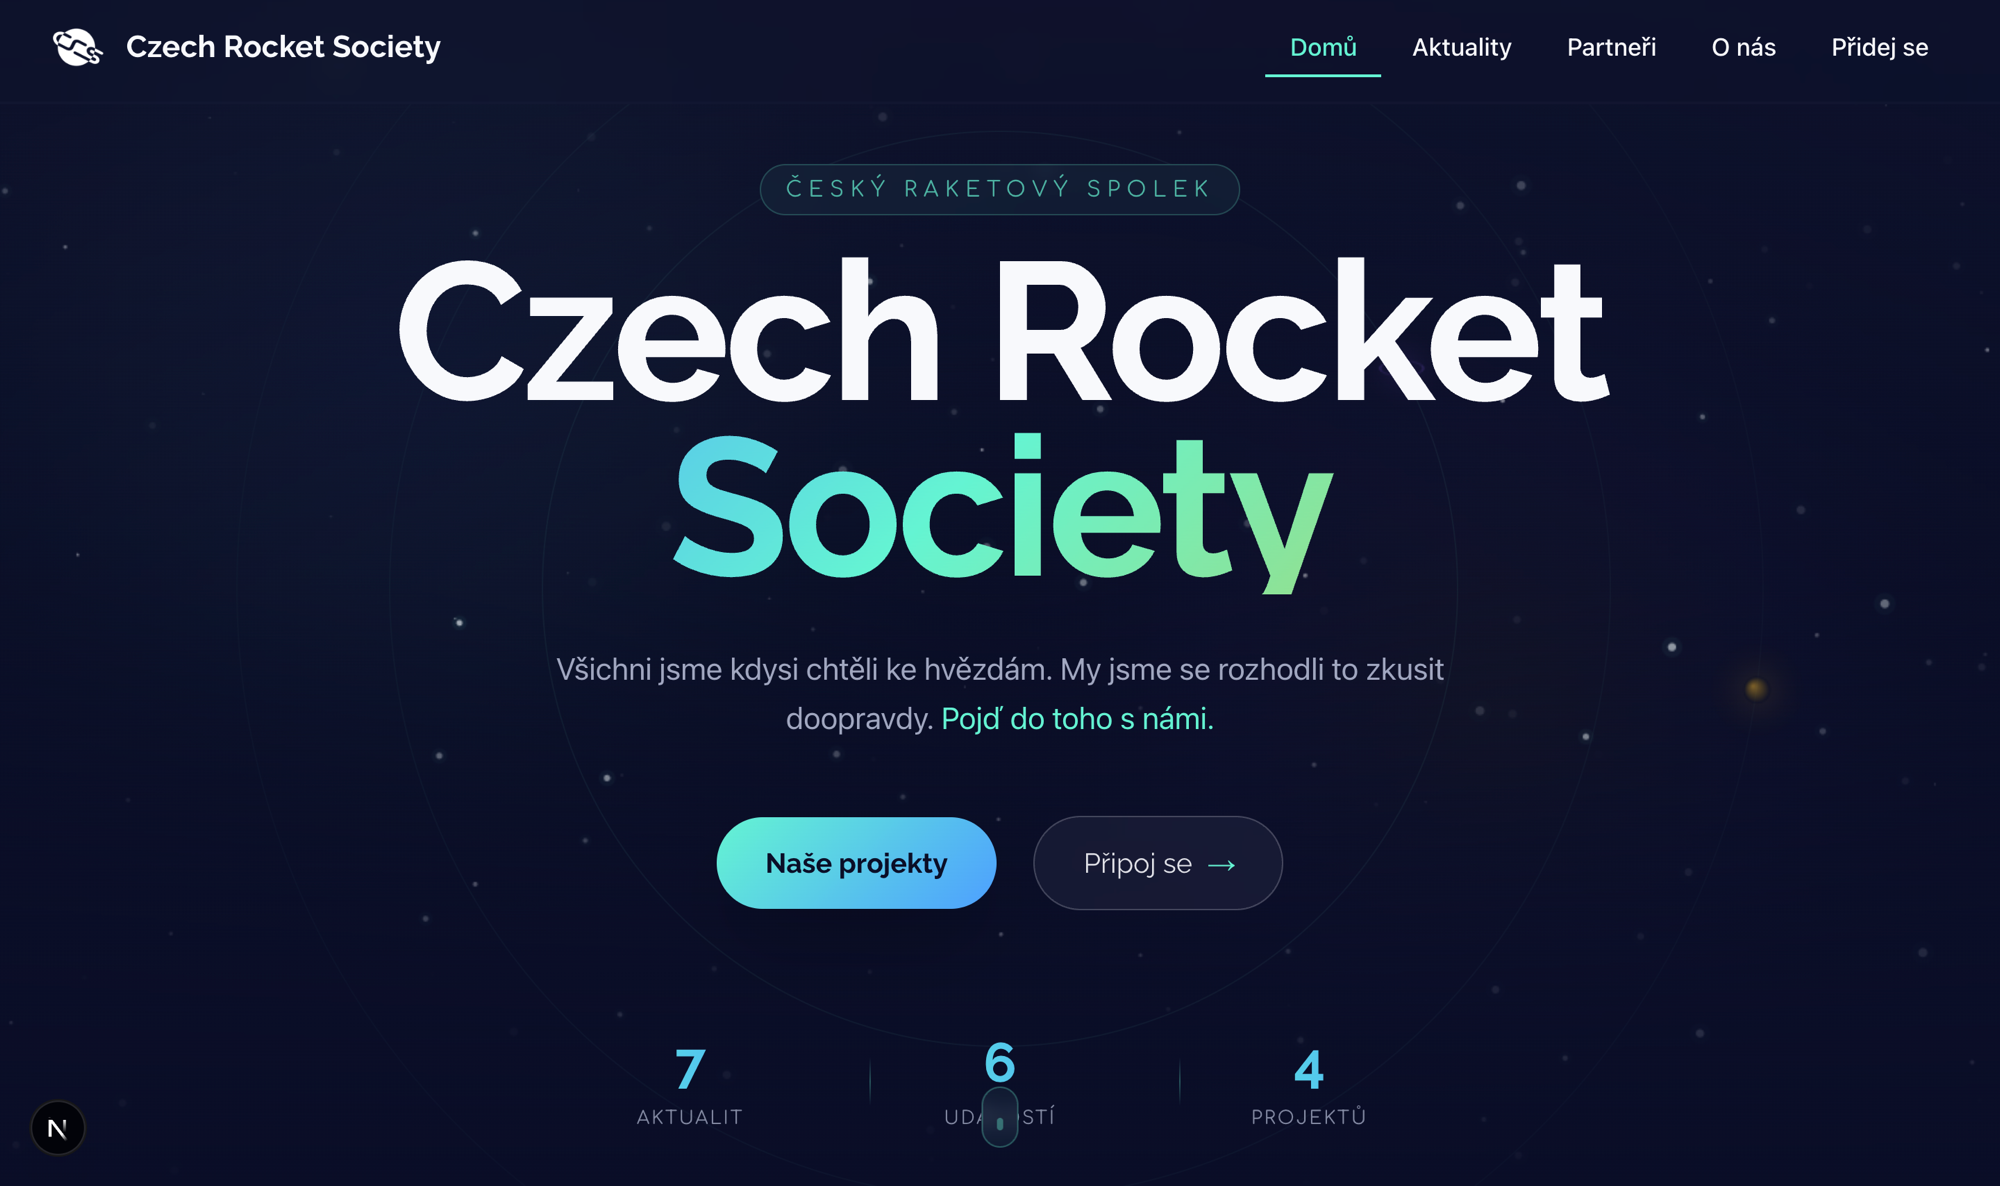
\includegraphics[width=\textwidth]{homepage.png}
\caption{Úvodní stránka veřejného webu Czech Rocket Society.}
\label{fig:appendix-homepage}
\end{figure}

\begin{figure}[H]
\centering
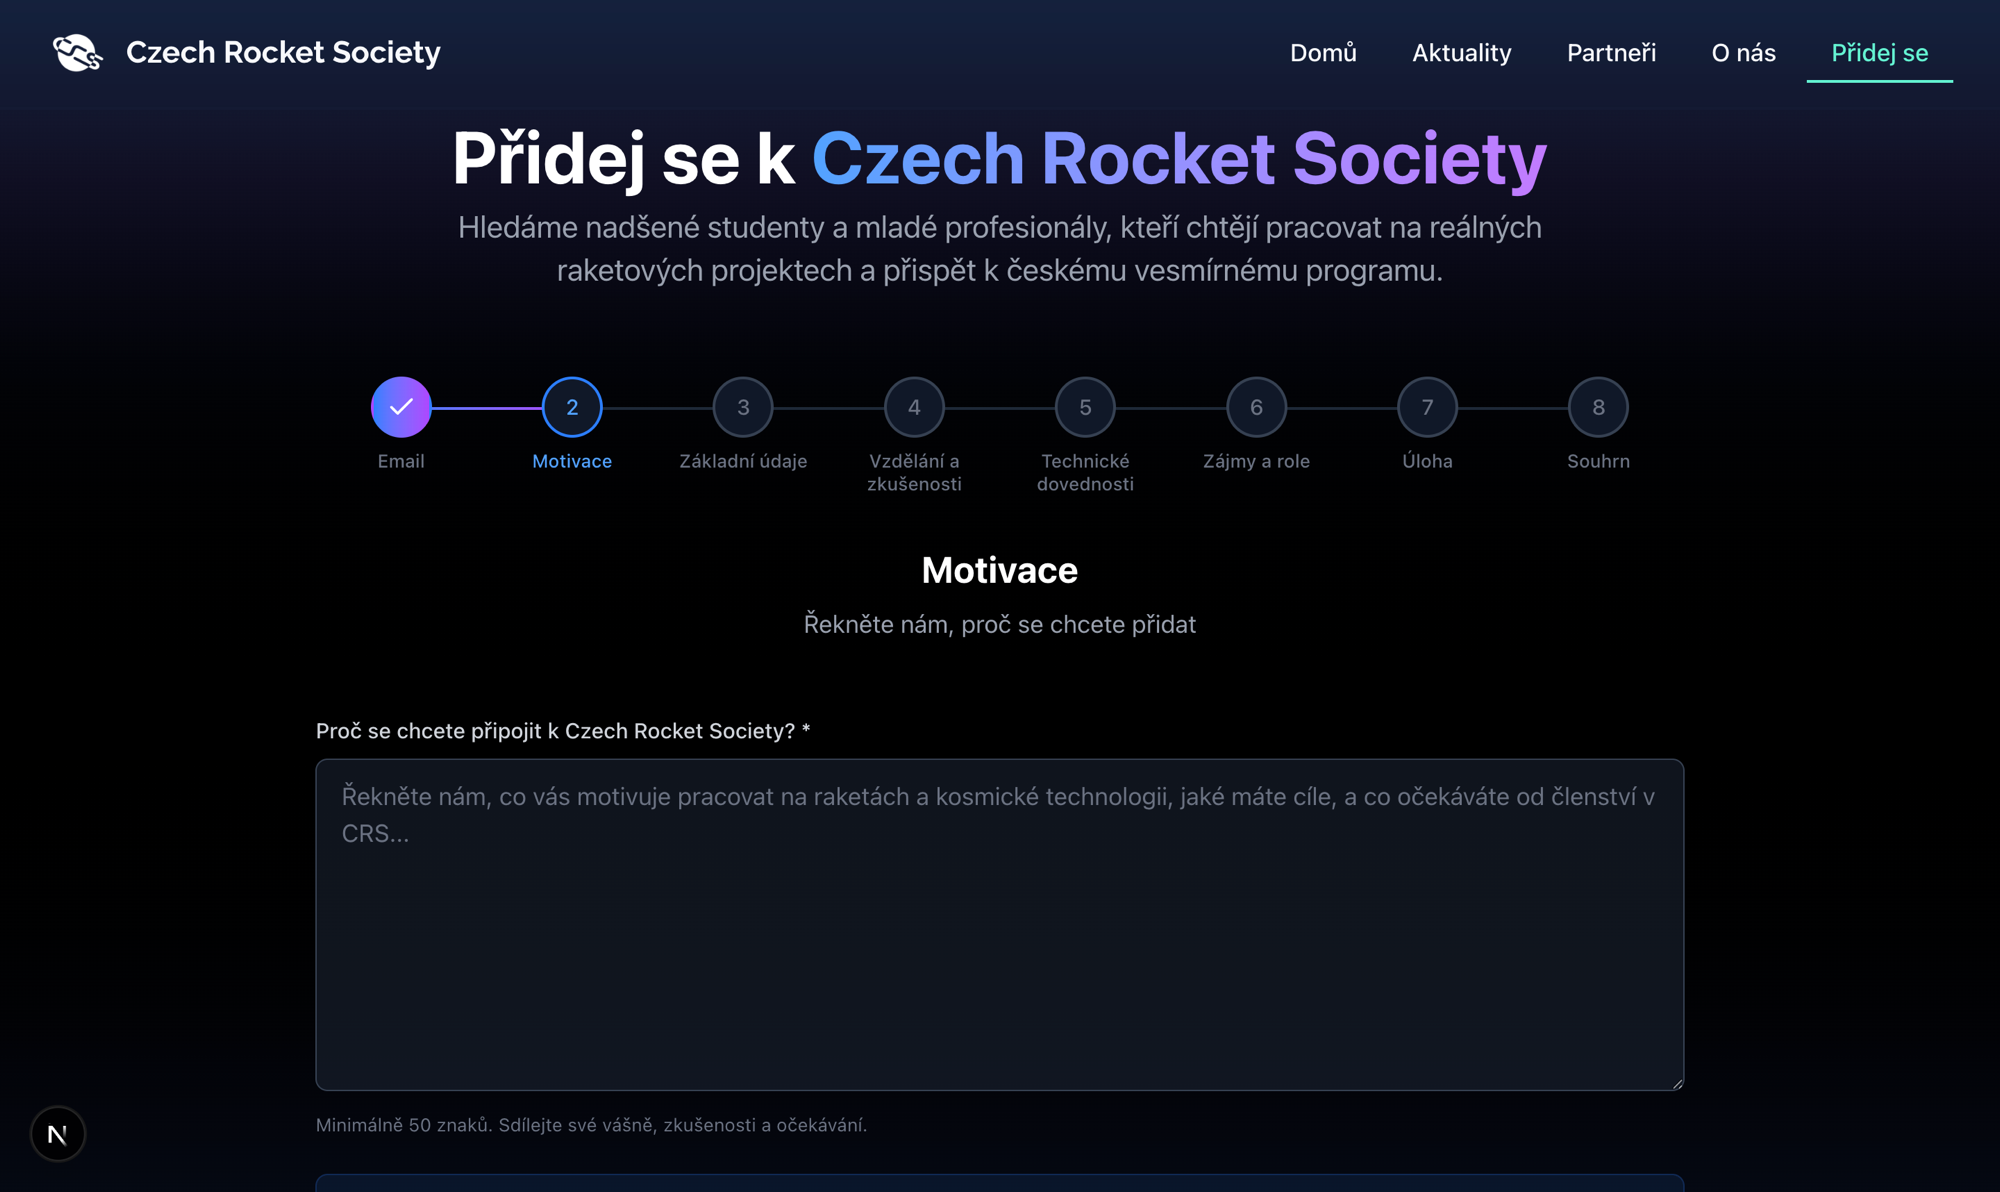
\includegraphics[width=\textwidth]{recruitment-form.png}
\caption{Náborový formulář -- ukázka jednoho z~kroků s~vizualizací postupu.}
\label{fig:appendix-recruitment}
\end{figure}

\begin{figure}[H]
\centering
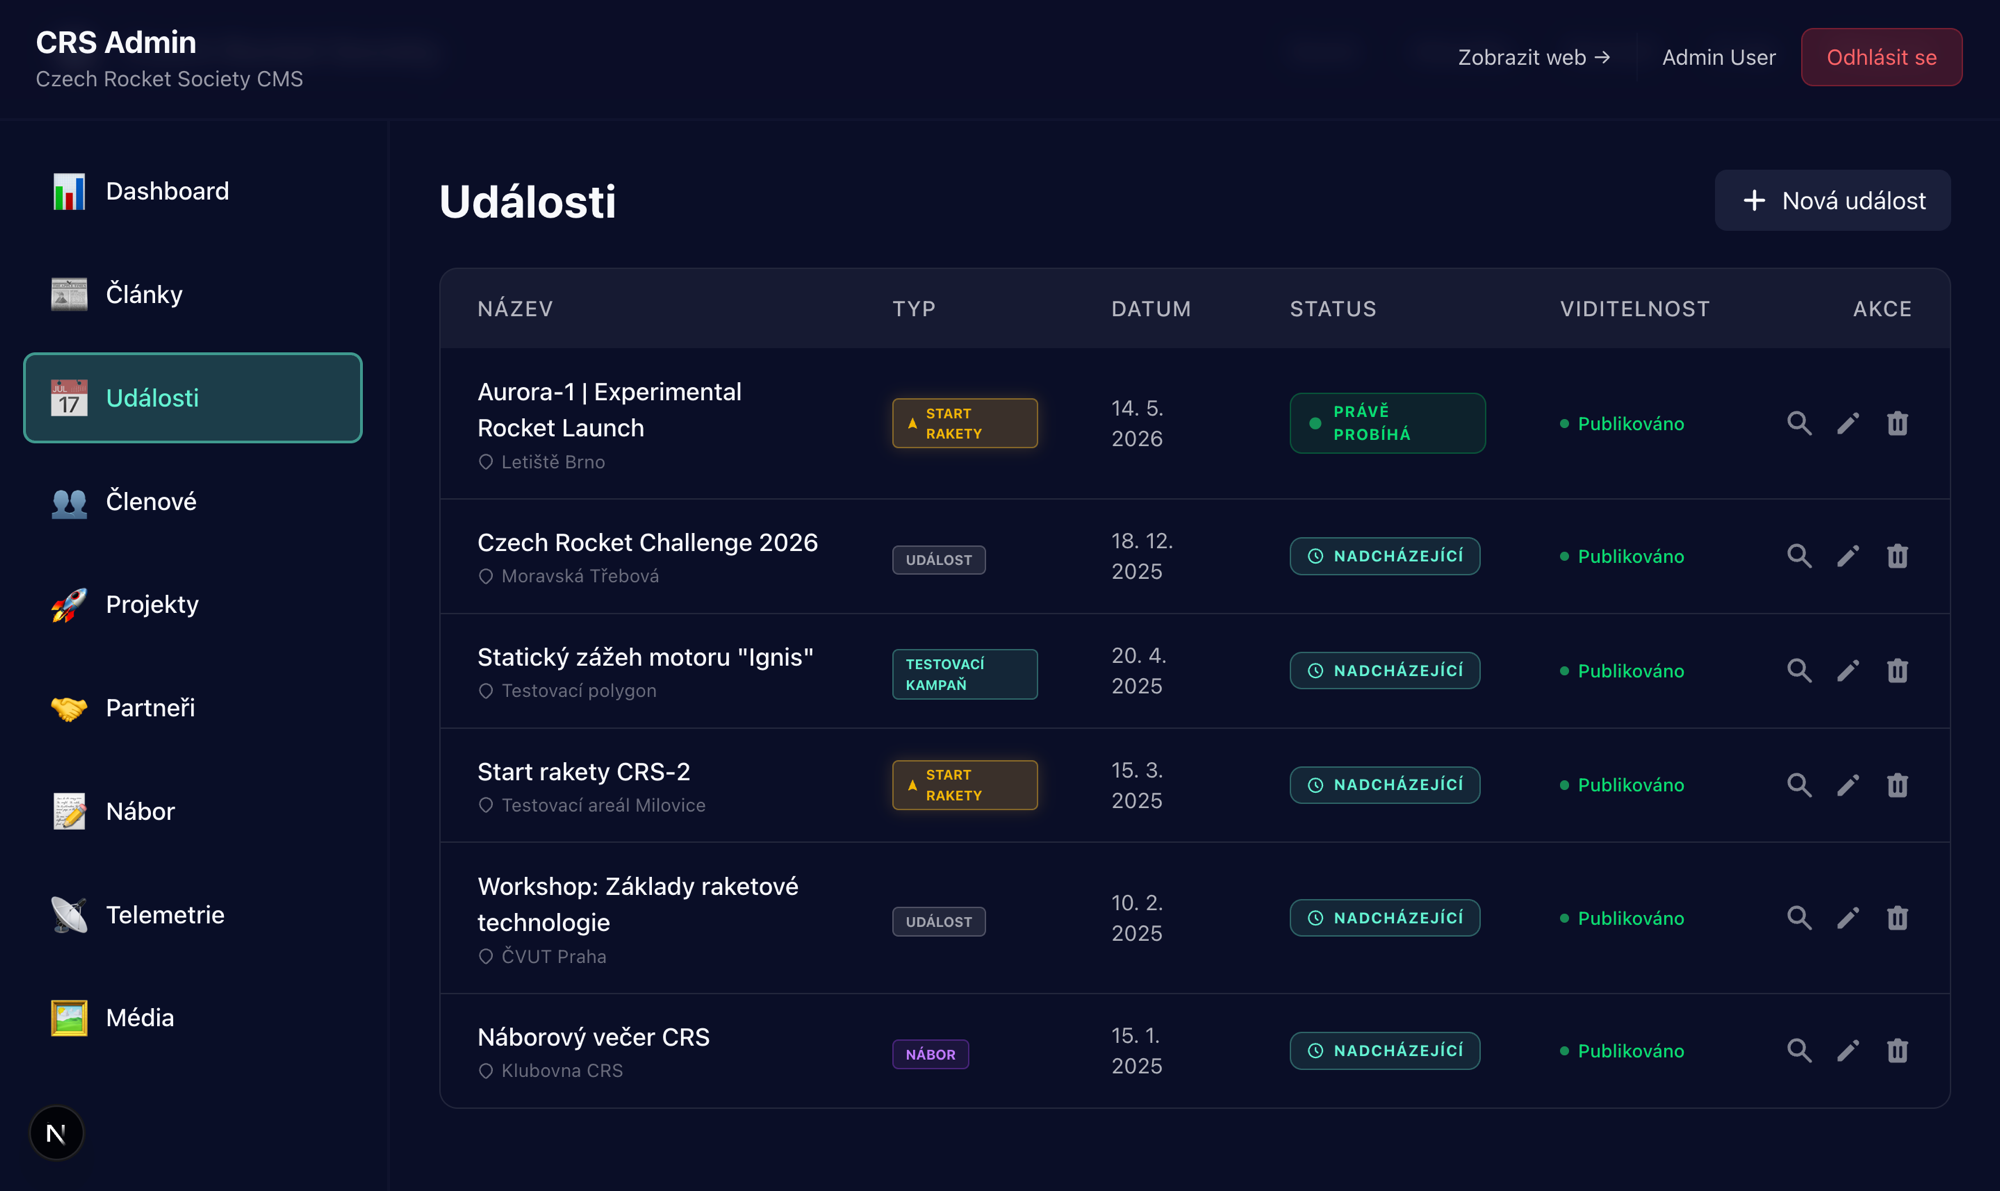
\includegraphics[width=\textwidth]{admin-events.png}
\caption{Administrační rozhraní -- správa událostí s~přehledem typů, statusů a~viditelnosti.}
\label{fig:appendix-admin-events}
\end{figure}

\begin{figure}[H]
\centering
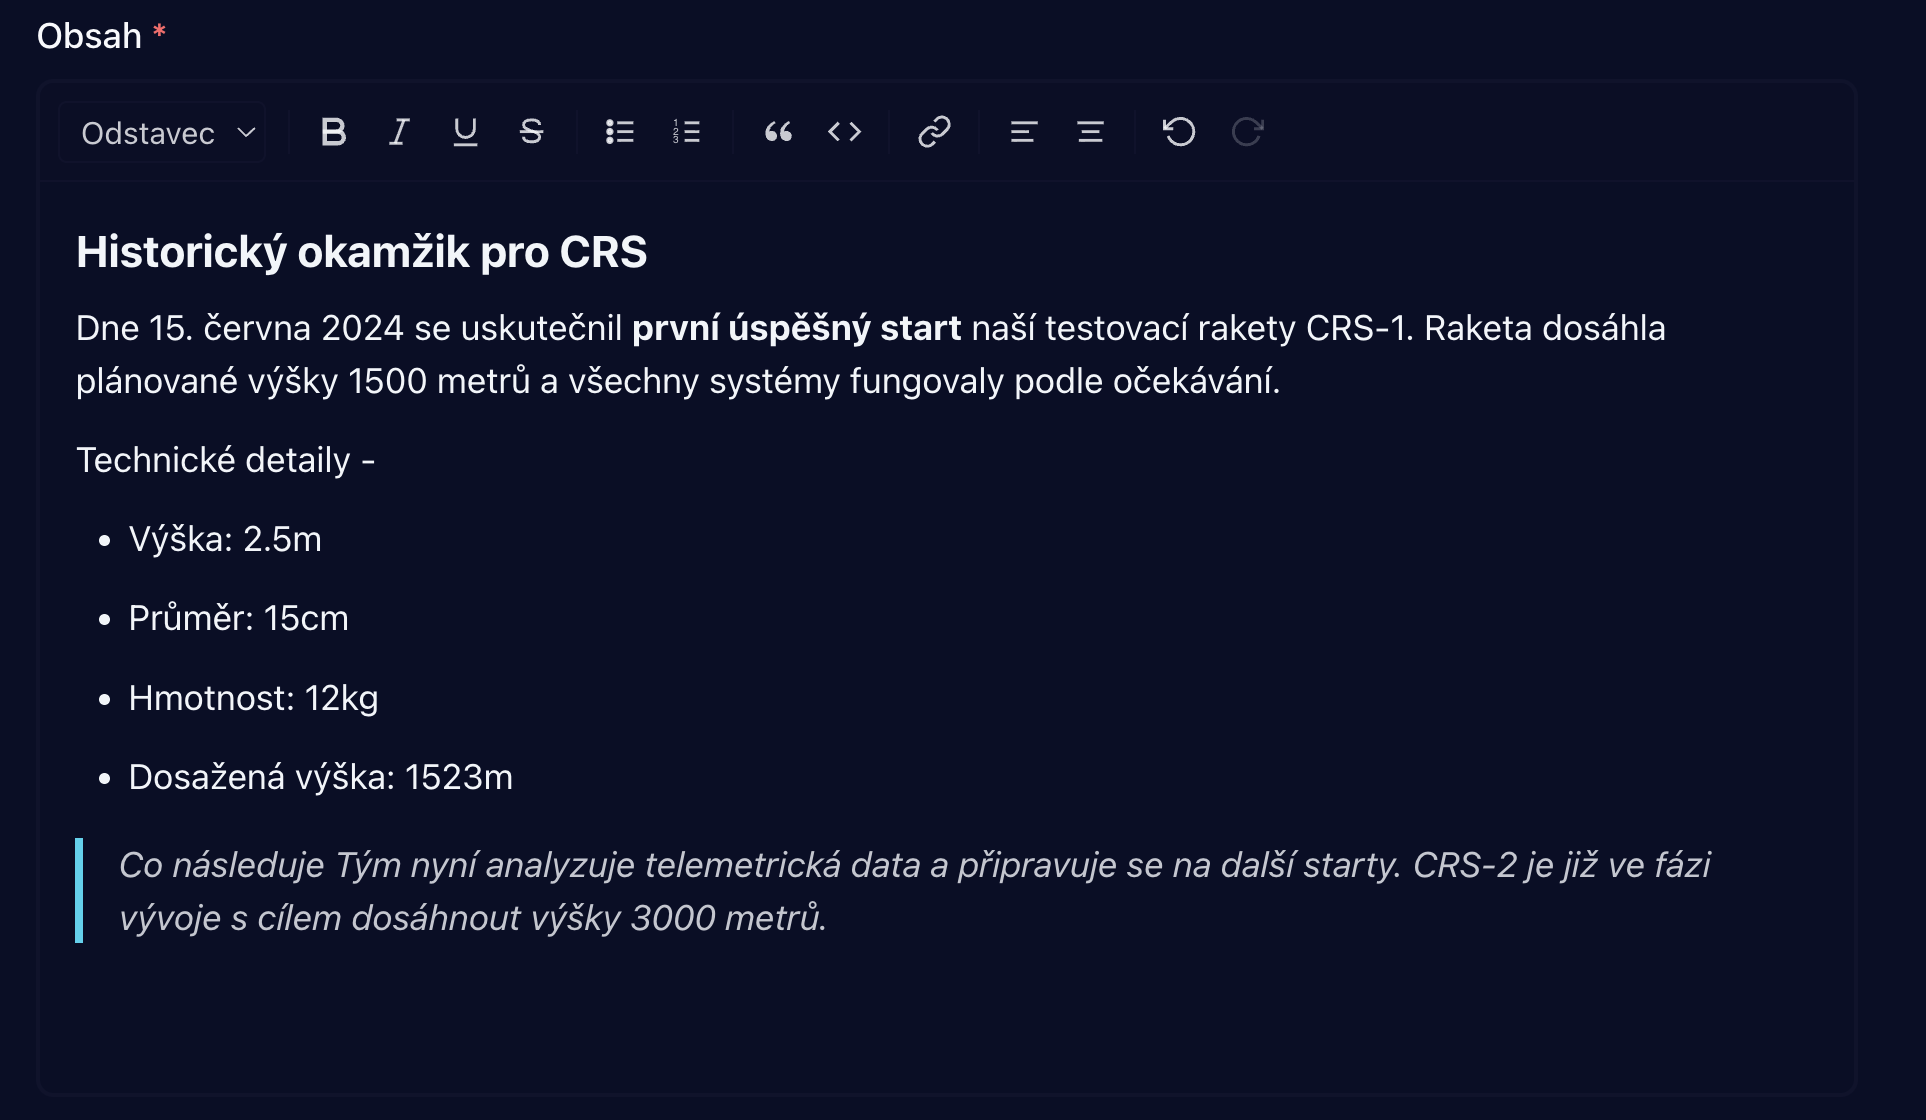
\includegraphics[width=\textwidth]{richtext-editor.png}
\caption{Rich-text editor Tiptap v~administraci s~formátovacím toolbarem.}
\label{fig:appendix-richtext}
\end{figure}

\begin{figure}[H]
\centering
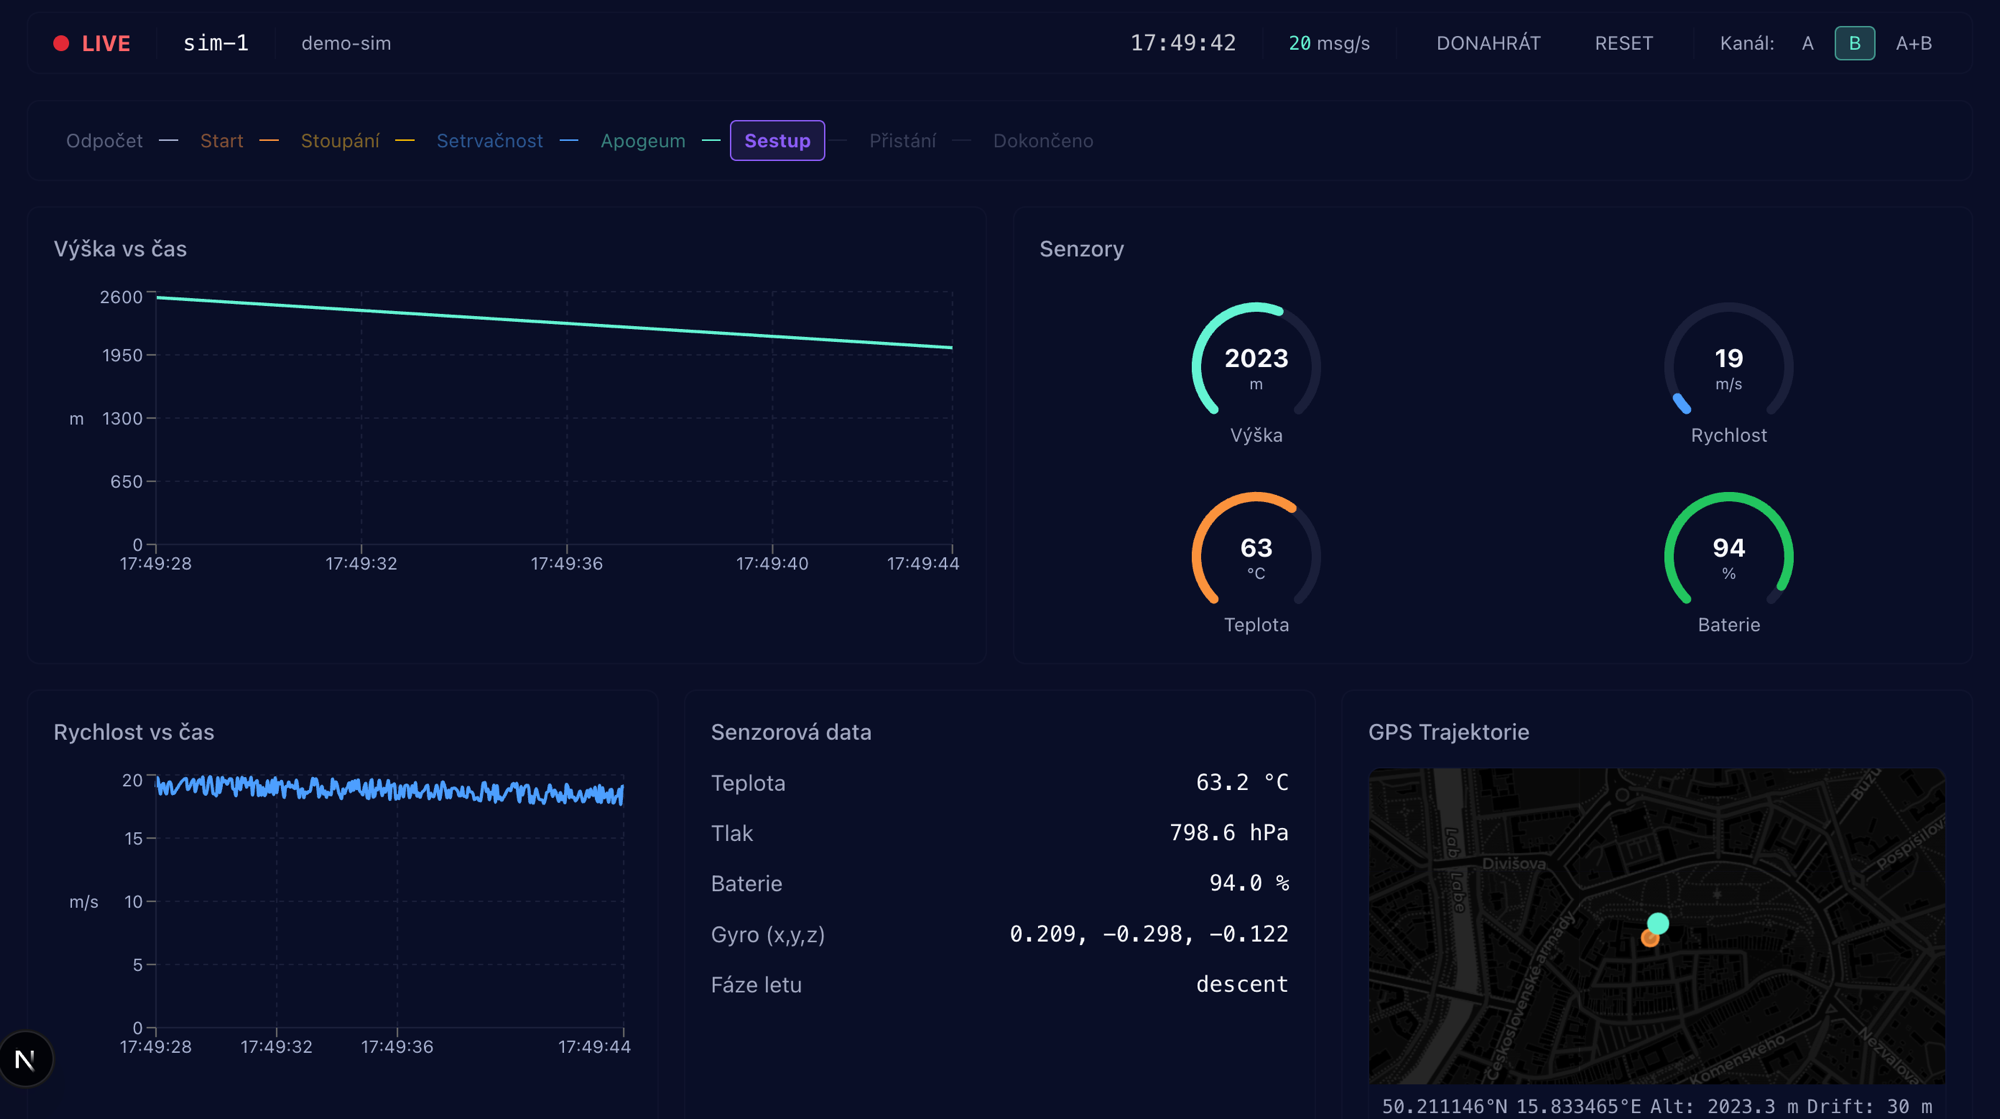
\includegraphics[width=\textwidth]{telemetry-live.png}
\caption{Telemetrický dashboard v~live režimu -- časové grafy, senzory, GPS trajektorie a~stavová lišta.}
\label{fig:appendix-telemetry}
\end{figure}

\chapter{Obsah přiloženého média}
\label{app:medium}

% TODO: Doplnit odkaz na GitHub repozitář

\noindent Repozitář obsahuje:
\begin{itemize}
    \item \texttt{apps/web/} -- zdrojový kód frontendové aplikace (Next.js)
    \item \texttt{apps/api/} -- zdrojový kód backendové aplikace (Hono)
    \item \texttt{apps/telemetry/} -- zdrojový kód telemetrického serveru (Go)
    \item \texttt{docker/} -- konfigurace Docker Compose a~služeb
    \item \texttt{thesis/} -- zdrojové soubory bakalářské práce (\LaTeX)
    \item \texttt{README.md} -- návod k~instalaci a~spuštění
\end{itemize}

\chapter{Zadání práce}
\label{app:zadani}

\noindent Originální zadání bakalářské práce z~informačního systému IS~STAG je vloženo na~následujících stránkách.

\includepdf[pages=-,pagecommand={},width=\textwidth]{images/zadani-stag.pdf}


\end{document}
